% Author: Alfredo Sánchez Alberca (asalber@ceu.es)
%----------------------------------------------------------------------------------------
%    DOCUMENT CLASS
%----------------------------------------------------------------------------------------

\documentclass[11pt,a4paper, openright]{book}
%----------------------------------------------------------------------------------------
%	PACKAGES AND OTHER DOCUMENT CONFIGURATIONS
%----------------------------------------------------------------------------------------

% Encoding settings
\usepackage[utf8]{inputenc}

% Language settings
\usepackage[spanish]{babel}

% Margins and layout
\usepackage[top=4cm, bottom=3cm, left=2.54cm, right=2.54cm]{geometry}

% Font settings
%\usepackage{type1cm}
\usepackage{pxfonts}

% Math support
\usepackage{amsmath} 

% Line breaking
\usepackage{microtype} 
\setlength{\emergencystretch}{2em}

% Graphics
\usepackage{graphicx}

% Arrays and tables
\usepackage{array}
\usepackage{multirow}

% Columns
\usepackage{multicol}

% Captions
\usepackage[margin=10mm,font=footnotesize,labelfont=bf]{caption}

% Pstricks
\usepackage[usenames,dvipsnames]{pstricks} % Postscript graphics
\usepackage{pst-all,pstricks-add,pst-math,pst-plot,pst-infixplot,pst-xkey}
\usepackage{pst-solides3d}
%\usepackage{pst-3dplot}
\usepackage{epsfig}

% Floating figures
\usepackage{subfigure}

% Lists
\usepackage[shortlabels]{enumitem} % Customize lists
%\setlist{nolistsep} % Reduce spacing between bullet points and numbered lists
\setlist[description]{style=sameline,leftmargin=0cm}

\makeatletter
\let\savees@listquot\es@listquot
\def\es@listquot{\protect\savees@listquot}
\makeatletter

\renewcommand{\theenumiii}{\arabic{enumiii}}

% Flush floating 
\usepackage{afterpage}

% hyperlinks
\usepackage[pdfauthor={Alfredo Sanchez Alberca}, pdftitle={Calculo aplicado con Derive},breaklinks,colorlinks=true]{hyperref}
\usepackage{breakurl}

% Indentation
%\setlength\parindent{0pt}

% Control of widow orphan lines
\clubpenalty=10000
\widowpenalty=10000 

% Caption formatting
\usepackage[margin=20pt, font=small, labelfont=bf, labelsep=endash]{caption}


% Color
\usepackage{xcolor} % Required for specifying colors by name
\definecolor{ocre}{RGB}{243,102,25} % Define the orange color used for highlighting throughout the book
\definecolor{blueceu}{RGB}{5,161,230} % Blue color of CEU logo
\definecolor{greenceu}{RGB}{185,209,16} % Green color of CEU logo
\definecolor{redceu}{RGB}{137,28,36} % Red color of CEU logo
\definecolor{grayceu}{RGB}{111,107,83} % Gray color of CEU logo
\definecolor{coral}{rgb}{1,0.5,0.31} % Orange color for graphics
\definecolor{royalblue1}{rgb}{0.28,0.46,1} % Blue color for graphics
\definecolor{mygreen}{rgb}{0,0.8,0} % Grtype filter texteen color for graphics

%----------------------------------------------------------------------------------------
%	VARIOUS REQUIRED PACKAGES
%----------------------------------------------------------------------------------------

\usepackage{tikz} % Required for drawing custom shapes
%\usepackage{booktabs} % Required for nicer horizontal rules in tables
\usepackage{eso-pic} % Required for specifying an image background in the title page

%----------------------------------------------------------------------------------------
%	SECTIONS AND SUBSECTIONS
%----------------------------------------------------------------------------------------
%\titleformat*{\section}{\Huge}
%\titleformat*{\subsection}{\Large}


% Chapter and section formatting 
\usepackage[rigidchapters,explicit]{titlesec}
\setlength{\fboxsep}{5pt}
\newlength{\titulolength}
\setlength{\titulolength}{\textwidth} 
\addtolength{\titulolength}{-2\fboxsep}
\addtolength{\titulolength}{-2\fboxrule}
\titleformat{\chapter}[display]
{\bfseries\sffamily}
{\filleft \mdseries \slshape \LARGE \color{blueceu} Práctica de Cálculo con Derive \Huge\thechapter}
{0.5ex}
{\colorbox{blueceu}{\parbox[t]{\titulolength}{\rule{0mm}{10mm}\Huge\sffamily\filleft\textcolor{white}{#1}}}}
\titleformat{\section}{\normalfont\Large\bfseries\color{blueceu}}{\arabic{section}}{1em}{#1}
\titleformat{\subsection}{\normalfont\large\bfseries\color{blueceu}}{\arabic{section}.\arabic{subsection}}{1em}{#1}
\titleformat{\subsubsection}{\normalfont\normalsize\bfseries\color{blueceu}}{\arabic{section}.\arabic{subsection}.\arabic{subsubsection}}{0.5em}{#1}
\titlespacing{\chapter}{0pt}{0pt}{30ex}
\titlespacing{\section}{0pt}{8ex}{4ex}

%----------------------------------------------------------------------------------------
%	MAIN TABLE OF CONTENTS
%----------------------------------------------------------------------------------------

% \usepackage{titletoc} % Required for manipulating the table of contents
% 
% \contentsmargin{0cm} % Removes the default margin
% % Chapter text styling
% \titlecontents{chapter}[1.25cm] % Indentation
% {\addvspace{15pt}\large\bfseries} % Spacing and font options for chapters
% {\color{gray}\contentslabel[\Large\thecontentslabel.]{1.25cm}} % Chapter number
% {}  
% {\color{gray}\bfseries\hfill\thecontentspage} % Page number
% % Section text styling
% \titlecontents{section}[1.25cm] % Indentation
% {\addvspace{5pt}\bfseries} % Spacing and font options for sections
% {\contentslabel[\thecontentslabel]{1.25cm}} % Section number
% {}
% {\hfill\color{black}\thecontentspage} % Page number
% []
% % Subsection text styling
% \titlecontents{subsection}[1.25cm] % Indentation
% {\addvspace{1pt}\small} % Spacing and font options for subsections
% {\contentslabel[\thecontentslabel]{1.25cm}} % Subsection number
% {}
% {\;\titlerule*[.5pc]{.}\;\thecontentspage} % Page number
% [] 

%----------------------------------------------------------------------------------------
%	MINI TABLE OF CONTENTS IN CHAPTER HEADS
%----------------------------------------------------------------------------------------

% % Section text styling
% \titlecontents{lsection}[0em] % Indendating
% {\footnotesize\sffamily} % Font settings
% {}
% {}
% {}
% 
% % Subsection text styling
% \titlecontents{lsubsection}[.5em] % Indentation
% {\normalfont\footnotesize\sffamily} % Font settings
% {}
% {}
% {}
 
%----------------------------------------------------------------------------------------
%	PAGE HEADERS
%----------------------------------------------------------------------------------------

% Headings and footers
\usepackage{fancyhdr}
\pagestyle{fancy}
\fancyhead{}
\renewcommand{\chaptermark}[1]{\markboth{\thechapter.\ #1}{}}
\fancyhead[LE]{\scshape Cálculo con Derive}
\fancyhead[RO]{\sffamily\slshape \leftmark}
\renewcommand{\headrulewidth}{0pt}
\renewcommand{\floatpagefraction}{.8}
\renewcommand{\textfraction}{.1} 


% \usepackage{fancyhdr} % Required for header and footer configuration
% 
% \pagestyle{fancy}
% \renewcommand{\chaptermark}[1]{\markboth{\color{grayceu}\sffamily\normalsize\textit{#1}}{}} % Chapter text font
% % settings
% %\renewcommand{\sectionmark}[1]{\markright{\color{grayceu}\sffamily\normalsize\textit{\thesection\hspace{5pt}#1}}{}} %
% % Section text font settings
% \fancyhf{} \fancyfoot[LE,RO]{\normalsize\thepage} % Font setting for the page number in the footer
% \fancyhead[RE]{{\color{grayceu}\sffamily\normalsize\textit{Pr�cticas de Bioestad�stica con R y RKTeaching}}} % Print the nearest
% % section name on the left side of odd pages
% \fancyhead[LO]{\leftmark} % Print the current chapter name on the right side of even pages
% \renewcommand{\headrulewidth}{0pt} % Removes the rule in the header
% \addtolength{\headheight}{2.5pt} % Increase the spacing around the header slightly
% \renewcommand{\footrulewidth}{0pt} % Removes the rule in the footer
% \fancypagestyle{plain}{\fancyhead{}\renewcommand{\headrulewidth}{0pt}} % Style for when a plain pagestyle is specified
% 
% % Removes the header from odd empty pages at the end of chapters
% \makeatletter
% \renewcommand{\cleardoublepage}{
% \clearpage\ifodd\c@page\else
% \hbox{}
% \vspace*{\fill}
% \thispagestyle{empty}
% \newpage
% \fi}


%----------------------------------------------------------------------------------------
%	THEOREM STYLES
%----------------------------------------------------------------------------------------

\usepackage{amsthm} % For including math equations, theorems, symbols, etc

\newcommand{\intoo}[2]{\mathopen{]}#1\,;#2\mathclose{[}}
\newcommand{\ud}{\mathop{\mathrm{{}d}}\mathopen{}}
\newcommand{\intff}[2]{\mathopen{[}#1\,;#2\mathclose{]}}
\newtheorem{notation}{Notation}[chapter]

\newtheoremstyle{blueceu} % Theorem style name
{7pt} % Space above
{7pt} % Space below
{\normalfont} % Body font
{} % Indent amount
{\small\bf\sffamily\color{blueceu}} % Theorem head font
{\;\;} % Punctuation after theorem head
{0.25em} % Space after theorem head
{\small\sffamily\color{blueceu}\thmname{#1}\thmnumber{\@ifnotempty{#1}{ }\@upn{#2}} % Theorem text (e.g. Theorem 2.1)
\thmnote{\ {\the\thm@notefont\sffamily\bfseries\color{blueceu}--- #3.}}} % Optional theorem note
\renewcommand{\qedsymbol}{$\blacksquare$} % Optional qed square

\newtheoremstyle{blacknumex} % Theorem style name
{7pt} % Space above
{7pt} % Space below
{\normalfont} % Body font
{} % Indent amount
{\small\bf\sffamily} % Theorem head font
{\;\;} % Punctuation after theorem head
{0.25em} % Space after theorem head
{\small\sffamily{\tiny\ensuremath{\blacksquare}}\ \thmname{#1}\thmnumber{\@ifnotempty{#1}{ }\@upn{#2}} % Theorem text (e.g. Theorem 2.1)
\thmnote{\ {\the\thm@notefont\sffamily\bfseries--- #3.}}} % Optional theorem note

\newtheoremstyle{blacknum} % Theorem style name
{7pt} % Space above
{7pt} % Space below
{\normalfont} % Body font
{} % Indent amount
{\small\bf\sffamily} % Theorem head font
{\;\;} % Punctuation after theorem head
{0.25em} % Space after theorem head
{\small\sffamily\thmname{#1}\thmnumber{\@ifnotempty{#1}{ }\@upn{#2}} % Theorem text (e.g. Theorem 2.1)
\thmnote{\ {\the\thm@notefont\sffamily\bfseries--- #3.}}} % Optional theorem note

\newtheoremstyle{example} % Theorem style name
{7pt} % Space above
{7pt} % Space below
{\normalfont} % Body font
{} % Indent amount
{\small\bf\sffamily} % Theorem head font
{\;\;} % Punctuation after theorem head
{0.25em} % Space after theorem head
{\small\sffamily\thmname{#1} % Theorem text (e.g. Theorem 2.1)
\thmnote{\ {\the\thm@notefont\sffamily\bfseries--- #3.}}} % Optional theorem note

\newtheoremstyle{indication} % Theorem style name
{-5pt} % Space above
{7pt} % Space below
{\normalfont} % Body font
{-28pt} % Indent amount
{\bf} % Theorem head font
{\kern-11.5pt} % Punctuation after theorem head
{20pt} % Space after theorem head
{\begin{tikzpicture}
\draw[anchor=west] (-26pt,10pt) node [fill=blueceu,opacity=1,inner
sep=1pt]{\Large\bfseries\textcolor{white}{\vphantom{plPQq}\makebox[17pt][c]{
\includegraphics[scale=0.3, trim=0 5mm 0 0]{img/bombilla}}}};
\end{tikzpicture}}
% Theorem text (e.g.
% Theorem 2.1)

\makeatother

% Defines the theorem text style for each type of theorem to one of the three styles above
\theoremstyle{ocrenum}
\newtheorem{proposicion}{Proposición}[chapter]
\newtheorem{problema}{Problema}[chapter]
\newtheorem{ejercicio}{Ejercicio}[chapter]
\theoremstyle{blacknumex}
\newtheorem{ejemplo}{Ejemplo}[chapter]
%\theoremstyle{blacknum}
\theoremstyle{blueceu}
\newtheorem{vocabulario}{Vocabulario}[chapter]
\newtheorem{definicion}{Definición}[chapter]
\newtheorem{teorema}{Teorema}[chapter]
\newtheorem{corolario}{Corolario}[chapter]
\theoremstyle{indication}
\newtheorem{indicacionT}{Indicación}
%\theoremstyle{example}
%\newtheorem{ejemplo}{Ejemplo}

%----------------------------------------------------------------------------------------
%	DEFINITION OF COLORED BOXES
%----------------------------------------------------------------------------------------

\RequirePackage[framemethod=default]{mdframed} % Required for creating the theorem, definition, exercise and corollary boxes

% Theorem box
\newmdenv[skipabove=7pt,
skipbelow=7pt,
backgroundcolor=black!5,
linecolor=ocre,
innerleftmargin=5pt,
innerrightmargin=5pt,
innertopmargin=5pt,
leftmargin=0cm,
rightmargin=0cm,
innerbottommargin=5pt]{tBox}

% Exercise box	  
\newmdenv[skipabove=7pt,
skipbelow=7pt,
rightline=false,
leftline=true,
topline=false,
bottomline=false,
backgroundcolor=ocre!10,
linecolor=ocre,
innerleftmargin=5pt,
innerrightmargin=5pt,
innertopmargin=5pt,
innerbottommargin=5pt,
leftmargin=0cm,
rightmargin=0cm,
linewidth=4pt]{eBox}	

% Definition box
\newmdenv[skipabove=10pt,
skipbelow=10pt,
rightline=false,
leftline=true,
topline=false,
bottomline=false,
linecolor=ocre,
innerleftmargin=5pt,
innerrightmargin=5pt,
innertopmargin=0pt,
leftmargin=0cm,
rightmargin=0cm,
linewidth=4pt,
innerbottommargin=0pt]{dBox}	

% Corollary box
\newmdenv[skipabove=7pt,
skipbelow=7pt,
rightline=false,
leftline=true,
topline=false,
bottomline=false,
linecolor=gray,
backgroundcolor=black!5,
innerleftmargin=5pt,
innerrightmargin=5pt,
innertopmargin=5pt,
leftmargin=0cm,
rightmargin=0cm,
linewidth=4pt,
innerbottommargin=5pt]{cBox}	

% Indication box
\newmdenv[skipabove=7pt,
skipbelow=7pt,
rightline=false,
leftline=true,
topline=false,
bottomline=false,
linecolor=blueceu,
backgroundcolor=black!5,
innerleftmargin=5pt,
innerrightmargin=5pt,
innertopmargin=5pt,
leftmargin=0pt,
rightmargin=0pt,
linewidth=4pt,
innerbottommargin=5pt]{iBox}				  
		  			  


% Creates an environment for each type of theorem and assigns it a theorem text style from the "Theorem Styles" section above and a colored box from above
\newenvironment{theorem}{\begin{tBox}\begin{theoremeT}}{\end{theoremeT}\end{tBox}}
\newenvironment{exercise}{\begin{eBox}\begin{exerciseT}}{\hfill{\color{ocre}\tiny\ensuremath{\blacksquare}}\end{exerciseT}\end{eBox}}				  
\newenvironment{definition}{\begin{dBox}\begin{definitionT}}{\end{definitionT}\end{dBox}}	
\newenvironment{example}{\begin{exampleT}}{\hfill{\tiny\ensuremath{\blacksquare}}\end{exampleT}}		
\newenvironment{corollary}{\begin{cBox}\begin{corollaryT}}{\end{corollaryT}\end{cBox}}	
\newenvironment{indicacion}{\begin{iBox}\begin{indicacionT}}{\end{indicacionT}\end{iBox}}	

%----------------------------------------------------------------------------------------
%	REMARK ENVIRONMENT
%----------------------------------------------------------------------------------------

%\newenvironment{remark}{\par\vskip10pt\small % Vertical white space above the remark and smaller font size
%\begin{list}{}{
%\leftmargin=35pt % Indentation on the left
%\rightmargin=25pt}\item\ignorespaces % Indentation on the right
%\makebox[-2.5pt]{\begin{tikzpicture}[overlay]
%\node[draw=ocre!60,line width=1pt,circle,fill=ocre!25,font=\sffamily\bfseries,inner sep=2pt,outer sep=0pt] at (-15pt,0pt){\textcolor{ocre}{R}};\end{tikzpicture}} % Orange R in a circle
%\advance\baselineskip -1pt}{\end{list}\vskip5pt} % Tighter line spacing and white space after remark

% %----------------------------------------------------------------------------------------
% %	SECTION NUMBERING IN THE MARGIN
% %----------------------------------------------------------------------------------------
% 
% \makeatletter
% %\renewcommand{\@seccntformat}[1]{\llap{\textcolor{grayceu}{\csname the#1\endcsname.}\hspace{1em}}}                    
% \renewcommand{\section}{
% 	\@startsection{section}{1}{\z@}
% 	{-4ex \@plus -1ex \@minus -.4ex}{1ex \@plus.2ex }
% 	{\normalfont\LARGE}
% }
% \renewcommand{\subsection}{
% 	\@startsection{subsection}{2}{\z@}
% 	{-3ex \@plus -0.1ex \@minus -.4ex}{0.5ex \@plus.2ex }
% 	{\normalfont\Large}
% }
% \renewcommand{\subsubsection}{
% 	\@startsection{subsubsection}{3}{\z@}
% 	{-2ex \@plus -0.1ex \@minus -.2ex}{0.2ex \@plus.2ex }
% 	{\normalfont\large}
% }                        
% \renewcommand{\paragraph}{
% 	\@startsection{paragraph}{4}{\z@}
% 	{-2ex \@plus-.2ex \@minus .2ex}{0.1ex}
% 	{\normalfont\bfseries}
% }
% 
% \def\thechapter{\arabic{chapter}}
% \def\thesection{\thechapter.\arabic{section}.}
% \def\thesubsection{\thesection\arabic{subsection}.}
% \def\thesubsubsection{\thesubsection\arabic{section}.}
% 
% %----------------------------------------------------------------------------------------
% %	CHAPTER HEADINGS
% %----------------------------------------------------------------------------------------
% %\newcommand{\thechapterimage}{}
% %\newcommand{\chapterimage}[1]{\renewcommand{\thechapterimage}{#1}}
% \def\@makechapterhead#1{
% \thispagestyle{empty}
% {
% \ifnum \c@secnumdepth >\m@ne
% \if@mainmatter
% \startcontents
% \begin{tikzpicture}[remember picture,overlay]
% % \node at (current page.north west)
% % {\begin{tikzpicture}[remember picture,overlay]
% % 
% % %\node[anchor=north west] at (-4pt,-27.5mm) {\includegraphics[width=\paperwidth]{\thechapterimage}};
% % %Commenting the 3 lines below removes the small contents box in the chapter heading
% % % \draw[fill=white,opacity=.6] (30mm,-30mm) rectangle (9cm,-9cm);
% % % \node[anchor=north west] at (30mm,-30mm) {\parbox[t][9cm][t]{5.5cm}{\huge\bfseries\flushleft \printcontents{l}{1}{\setcounter{tocdepth}{2}}}};
% % % \draw[anchor=west] (5cm,-11cm) node [rounded corners=25pt,fill=white,opacity=.7,inner sep=15.5pt]{\huge\sffamily\bfseries\textcolor{black}{\vphantom{plPQq}\makebox[20cm]{}}};
% \draw[anchor=north west, fill=black] (0mm,50mm) rectangle (1pt,10mm);
% \draw[anchor=north west] (0cm,20mm) node {\scalebox{1.5}{\Huge{\textcolor{grayceu}\thechapter}}}; 
% %\draw[anchor=west] (0cm,0cm) node {\Huge{#1}}; 
% \end{tikzpicture}
% \par\vspace*{2cm}
% {\Huge #1}
% \par\vspace*{1cm}
% % \end{tikzpicture}}\par\vspace*{230\p@}
% }}
% \def\@makeschapterhead#1{
% \thispagestyle{empty}
% {
% \ifnum \c@secnumdepth >\m@ne
% \if@mainmatter
% \startcontents
% \begin{tikzpicture}[remember picture,overlay]
% % \node at (current page.north west)
% % {\begin{tikzpicture}[remember picture,overlay]
% % \node[anchor=north west] at (-4pt,-27.5mm) {\includegraphics[width=\paperwidth]{\thechapterimage}};
% % \draw[anchor=west] (5cm,-11cm) node [rounded corners=25pt,fill=white,opacity=.7,inner sep=15.5pt]{\huge\sffamily\bfseries\textcolor{black}{\vphantom{plPQq}\makebox[20cm]{}}};
% % \draw[anchor=west] (5cm,-11cm) node [rounded corners=25pt,inner sep=15.5pt]{\huge\sffamily\bfseries\textcolor{black}{#1\vphantom{plPQq}\makebox[20cm]{}}};
% % \end{tikzpicture}};
% % \end{tikzpicture}}\par\vspace*{230\p@}
% %\draw[anchor=west] (0cm,0cm) node {\Huge{#1}}; 
% \end{tikzpicture}
% {\Huge #1}
% \par\vspace*{1cm}
% }}
% \makeatother

 % Insert the commands_book.tex file which contains the majority of the structure behind the template

%----------------------------------------------------------------------------------------
%	COMMANDS FOR INDICATIONS
%----------------------------------------------------------------------------------------
\usepackage{menukeys}
\renewmenumacro{\menu}[>]{paths}
%\newmenustylesimple*{botonstyle}{\textbf{\CurrentMenuElement}}
%\renewmenumacro{\keys}{botonstyle}
\newcommand{\boton}[1]{\textsf{\small #1}}
\newcommand{\opcion}[1]{\textsf{\small #1}}
\newcommand{\campo}[1]{\textsf{\small #1}}
\newcommand{\comando}[1]{\texttt{#1}}
\newcommand{\variable}[1]{\textsf{\small #1}}
\newcommand{\resultado}[1]{\texttt{#1}}


%----------------------------------------------------------------------------------------
%	HYPHENATION
%----------------------------------------------------------------------------------------
\hyphenation{}

% OTHERS
\newcommand{\resetcounters}{\setcounter{page}{1} \setcounter{section}{0} \setcounter{footnote}{0} \setcounter{figure}{0} \setcounter{table}{0}}

% MATH OPERATORS IN SPANISH
\newcommand{\sen}{\operatorname{sen}}
\newcommand{\arcsen}{\operatorname{arcsen}}
\newcommand{\tg}{\operatorname{tg}}
\newcommand{\arctg}{\operatorname{arctg}}
\newcommand{\cosec}{\operatorname{cosec}}
\newcommand{\cotg}{\operatorname{cotg}}
\newcommand{\dom}{\operatorname{Dom}}
\newcommand{\im}{\operatorname{Im}}
\newcommand{\dint}{\displaystyle \int}

%========================================================================================
%   DOCUMENT BODY
%========================================================================================
\begin{document}
\frontmatter 
% Add two blank pages at the begining
%\null\thispagestyle{empty}\newpage
%\null\thispagestyle{empty}\newpage
%----------------------------------------------------------------------------------------
%	TITLE PAGE
%----------------------------------------------------------------------------------------
\begin{titlepage}
% \AddToShipoutPictureBG*{\includegraphics[width=\paperwidth,height=\paperheight]{img/portada}}
% \clearpage
% \thispagestyle{empty}
% \end{titlepage}
% 
% \null\newpage
% \thispagestyle{empty}
% 
% \null\newpage
\thispagestyle{empty}
%\thispagestyle{empty}
\vspace*{7cm}
\par

% Book title
\begin{center}
\normalfont\fontsize{30}{30}\selectfont
{\bfseries \color{blueceu}Cálculo con Derive}
\end{center}
%\vspace*{5mm}
%\hrule
\vspace{1cm}
% Authors names
\begin{center}
\Large
\begin{tabular}{c}
Santiago Angulo Díaz-Parreño (\url{sangulo@ceu.es})\\
Juan Carlos Garro Garro (\url{garro.eps@ceu.es})\\
Eduardo López Ramírez (\url{elopez@ceu.es})\\
José Rojo Montijano (\url{jrojo.eps@ceu.es})\\
Anselmo Romero Limón (\url{arlimon@ceu.es})\\
Alfredo Sánchez Alberca (\url{asalber@ceu.es})\\
Susana Victoria Rodríguez (\url{victoria.eps@ceu.es})
%\url{http://aprendeconalf.es}
\end{tabular}

\medskip 
Departamento de Matemática Aplicada y Estadística\\ CEU San Pablo\\[1cm]
\medskip 
Septiembre 2016

\vspace{1cm}

\includegraphics[height=3cm]{img/logo_uspceu}
\end{center}
\vfill
\end{titlepage} 

%----------------------------------------------------------------------------------------
%	COPYRIGHT PAGE
%----------------------------------------------------------------------------------------
% Términos de la licencia Creative Commons 2.5
\begin{titlepage}
\null
\vfill
\hrule depth 3pt
\smallskip
\sffamily

\noindent \textbf{Prácticas de Cálculo con Derive}\\
Santiago Angulo Díaz-Parreño, José Rojo Montijano, Anselmo Romero Limón y Alfredo Sánchez Alberca.

\bigskip
\begin{center}

\includegraphics[scale=0.1]{img/cc-logo}
\end{center}

\small
Esta obra está bajo una licencia Reconocimiento­-No comercial-­Compartir bajo la 
misma licencia 2.5 España de Creative Commons. Para ver una copia de esta 
licencia, visite http://creativecommons.org/licenses/by­nc­sa/2.5/es/ o envie una 
carta a Creative Commons, 171 Second Street, Suite 300, San Francisco, California 
94105, USA.

\medskip
Con esta licencia eres libre de:
\begin{itemize}
\item Copiar, distribuir y mostrar este trabajo.
\item Realizar modificaciones de este trabajo.
\end{itemize}

Bajo las siguientes condiciones:
\begin{center}
\begin{tabular}{ccp{10cm}}

\includegraphics[scale=0.2]{img/cc-by} & \qquad & \textbf{Reconocimiento}. Debe reconocer los créditos de la obra de la manera especificada por el autor o el licenciador (pero no de una manera que sugiera que tiene su apoyo o apoyan el uso que hace de su obra).\\

\includegraphics[scale=0.2]{img/cc-e} & \qquad & \textbf{No comercial}. No puede utilizar esta obra para fines comerciales.\\

\includegraphics[scale=0.2]{img/cc-c} & \qquad & \textbf{Compartir bajo la misma licencia}. Si altera o transforma esta obra, o genera una obra derivada, sólo puede distribuir la obra generada bajo una licencia idéntica a ésta.
\end{tabular}
\end{center}

\begin{itemize}
\item Al reutilizar o distribuir la obra, tiene que dejar bien claro los términos de la licencia de esta obra.
\item Alguna de estas condiciones puede no aplicarse si se obtiene el permiso del titular de los derechos de autor
\item Nada en esta licencia menoscaba o restringe los derechos morales del autor.
\end{itemize}

\hrule depth 3pt
\end{titlepage}

%----------------------------------------------------------------------------------------
%	TABLE OF CONTENTS
%----------------------------------------------------------------------------------------
%\chapterimage{img/chapter_head.png} % Table of contents heading image
{\pagestyle{plain} % No headers
%\input{registro}
\tableofcontents\thispagestyle{empty}
  % Print the table of contents itself
\cleardoublepage % Forces the first chapter to start on an odd page so it's on the right
}

\mainmatter 
%----------------------------------------------------------------------------------------
%	CHAPTERS
%----------------------------------------------------------------------------------------
% Author: Alfredo Sánchez Alberca (asalber@ceu.es)
\chapter{Introducción a Derive}

\section{Introducción}
La gran potencia de cálculo alcanzada por los ordenadores en las
últimas décadas, ha convertido a los mismos en poderosas
herramientas al servicio de todas aquellas disciplinas que, como las
matemáticas, requieren cálculos largos y complejos.

Derive$^{\textsf{\textregistered}}$
\renewcommand{\thefootnote}{\fnsymbol{footnote}}\footnote{Esta
practica está basada en la versión 6.1 de
Derive$^{\textregistered}$ para Windows en castellano.} es uno de
los programas de cálculo numérico y simbólico más utilizados.
Aparte de sus capacidades el cálculo numérico, vectorial y
matricial, también permite realizar representaciones gráficas, lo
cual permite resolver multitud de problemas de álgebra, análisis,
cálculo, geometría e incluso estadística. La ventaja de Derive
frente a otros programas habituales de cálculo como Mathematica,
Mapple o MATLAB, radica en su sencillez y simplicidad de uso, lo
cual lo hace idóneo para la enseñanza de las matemáticas.

\begin{center}
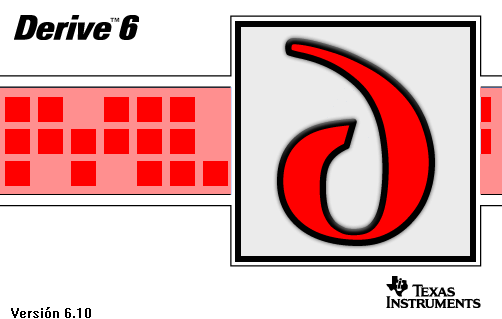
\includegraphics[scale=0.6]{img/introduccion_derive/introduccion}
\end{center}


El objetivo de esta práctica es introducir al alumno en la
utilización de este programa, enseñándole a realizar las operaciones
básicas más habituales.


\section{Funciones básicas}
\subsection*{Arranque}
Como cualquier otra aplicación de Windows, para arrancar el programa
hay que pulsar sobre la opción correspondiente del menú
\menu{Inicio>Programas}, o bien sobre el icono de escritorio


\begin{center}

\includegraphics[scale=0.4]{img/introduccion_derive/icono}
\end{center}

Cuando el programa arranca, en la pantalla aparece la ventana
principal del programa que se conoce como \emph{ventana de Álgebra}
(figura \ref{g:principal}).

\begin{figure}[h!]
\begin{center}
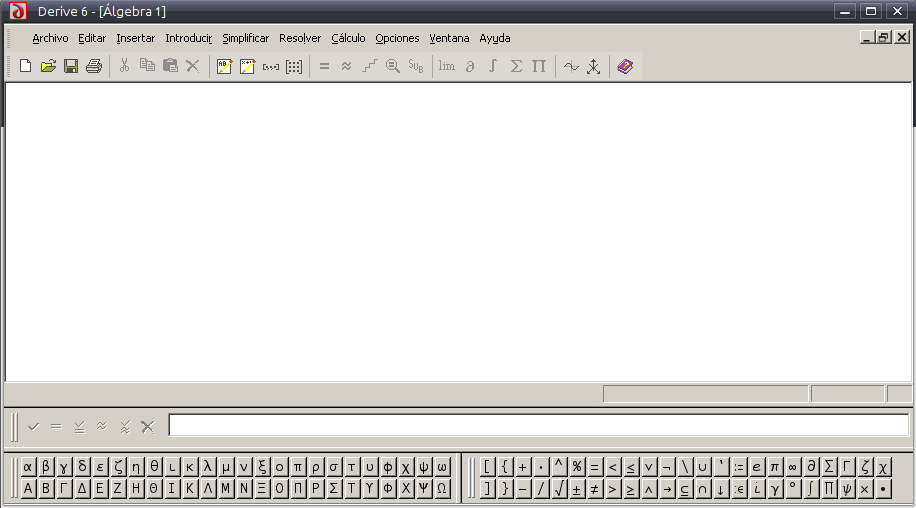
\includegraphics[scale=0.6]{img/introduccion_derive/principal}
\caption{Ventana principal de Derive.} \label{g:principal} 
\end{center}
\end{figure}


Como cualquier otra ventana de aplicación de Windows, la ventana
principal tiene una barra de título, una barra de menús con las
distintas funciones que puede hacer Derive (cálculo de límites,
derivadas, integrales, representaciones gráficas, etc.), una barra
de botones que son atajos a las opciones más habituales de los
menús, y una barra de estado en la parte inferior que nos indica lo
que hace el programa en cada instante. Además, por defecto, en la
parte inferior de la ventana aparece el editor de expresiones, que
pasamos a describir a continuación.

\subsection*{Edición de expresiones}
Antes de realizar cualquier cálculo sobre una expresión matemática,
lo primero es escribir dicha expresión y aprender a manipularla.
\subsection*{Introducción de expresiones}
Para introducir una expresión se utiliza el editor de expresiones
(figura~\ref{g:editor}), el cual aparece directamente en la parte
baja de la ventana de Álgebra.
\begin{figure}[h!]
\begin{center}
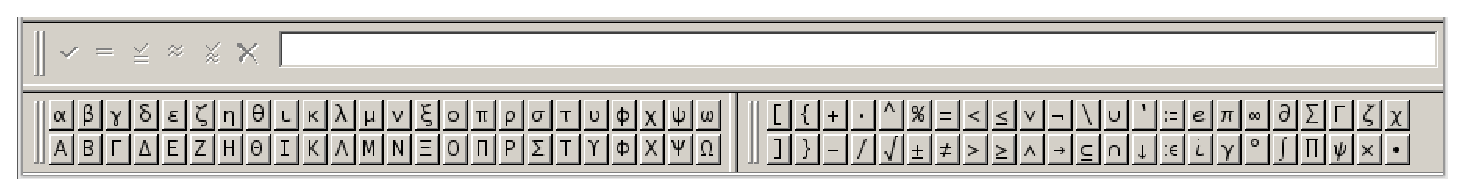
\includegraphics[scale=0.6]{img/introduccion_derive/authorexpression}
\caption{Editor de expresiones.} \label{g:editor} 
\end{center} 
\end{figure}

El editor de expresiones está compuesto por una línea de edición,
que se utiliza para dar forma a las expresiones matemáticas (también
permite introducir comentarios de texto) que vamos a utilizar con el
programa, una barra con las letras del alfabeto griego, a menudo
presentes en las expresiones matemáticas, y una barra de símbolos
matemáticos con los operadores más habituales (suma, resta,
producto, división, paréntesis, raíz cuadrada) y las constantes que
más se utilizan (número $e$, número $\pi$...).

En el editor de expresiones podemos escribir números, letras (que
serán variables), símbolos y operadores aritméticos y relacionales.
Los operadores más habituales en la construcción de expresiones son
los que aparecen en la siguiente tabla:

\begin{center}
\begin{tabular}{|c|c|}
\hline
 Símbolo &   Operador   \\
\hline\hline
    \texttt{+}    &     suma     \\
\hline
    \texttt{-}    &    resta     \\
\hline
    \texttt{*}    &   producto   \\
\hline
    \texttt{/}    &   cociente   \\
\hline
   \texttt{\^{}}    & potenciación \\
\hline
\end{tabular}
\end{center}

A la hora de escribir una expresión hay que tener en cuenta que
Derive tiene establecido un orden de prioridad en la evaluación de
los operadores. En primer lugar evalúa las funciones y constantes
predefinidas, después evalúa las potencias, después productos y
cocientes (ambos con igual prioridad y de izquierda a derecha), y
por último sumas y restas (ambas con igual prioridad y de izquierda
a derecha). Para forzar la evaluación de una subexpresión,
saltándose el orden de evaluación de Derive, se utilizan paréntesis.
Así, como se ve en el siguiente ejemplo, dependiendo de cómo se
introduzca una expresión pueden obtenerse resultados diferentes.

\begin{center}\renewcommand{\arraystretch}{2}
\begin{tabular}{|c|c|}
\hline
  Expresión introducida & Expresión resultante \\
\hline\hline
        \texttt{4x-1/x-5}        & $4x-\dfrac{1}{x}-5$ \\
\hline
       \texttt{(4x-1)/x-5}       & $\dfrac{4x-1}{x}-5$  \\
\hline
       \texttt{4x-1/(x-5)}       & $4x-\dfrac{1}{x-5}$  \\
\hline
      \texttt{(4x-1)/(x-5)}      & $\dfrac{4x-1}{x-5}$  \\
\hline
\end{tabular}
\end{center}

Cada vez que introducimos una expresión, esta aparece en la ventana
de Algebra etiquetada con un número precedido del símbolo de
almoadilla \verb"#", tal y como se muestra en la
figura~\ref{g:expresiones}. Posteriormente, cada vez que queramos
hacer referencia a dicha expresión podremos utilizar su etiqueta en
lugar de volver a escribir la expresión.

Es posible seleccionar cualquier expresión o subexpresión de la
ventana Algebra con el ratón o bien con las teclas del cursor.

La tecla \texttt{F3} permite introducir la expresión que tengamos
seleccionada en el editor de expresiones.

\subsubsection*{Modificación de expresiones}
Una vez introducida una expresión, podemos volver a editarla para
realizar cualquier corrección o cambio mediante el menú
\menu{Editar>Expresión} y aparecerá la ventana del editor de
expresiones con la expresión seleccionada.
\subsubsection*{Eliminación de expresiones}
Para eliminar una expresión de la ventana de Algebra, basta con
seleccionarla y utilizar el menú \menu{Editar>Borrar} y la
expresión seleccionada desaparecerá automáticamente, mientras que el
resto de las expresiones se renumeran automáticamente. También es
posible eliminar bloques completos de expresiones consecutivas
seleccionando previamente el bloque de expresiones a eliminar.

\textbf{¡Importante!}: Si hemos eliminado alguna expresión por
equivocación, es posible recuperarla mediante el menú
\menu{Editar>Recuperar}.

\subsubsection*{Reordenación de expresiones}
Es posible cambiar la posición que ocupa una expresión en la ventana
de Álgebra marcándola y arrastrándola mediante el ratón hasta la
posición que queremos que ocupe. Al cambiar la posición de una
expresión, inmediatamente se renumeran las expresiones de la ventana
de Álgegra.

\subsubsection*{Introducción de comentarios}
Hay dos formas diferentes para introducir un comentario en la
secuencia de expresiones. La primera consiste en utilizar la línea
de edición escribiendo el texto del comentario entre comillas, y,
si procedemos de esta manera, el comentario aparecerá como una
expresión más, con su correspondiente etiqueta de ordenación. La
segunda es mediante el menú \menu{Insertar>Objeto de Texto}, y
de esta forma el comentario aparece sin etiqueta de ordenación ya
que se trata de un objeto más insertado en el archivo, como
también lo sería una gráfica, un dibujo, una fotografía o una hoja
de cálculo...

\subsubsection*{Nombres de variables}
Por defecto Derive utiliza una sola letra para representar una
variable, de manera que la expresión \texttt{xy}, no se interpreta
como una variable de nombre $xy$, sino como el producto de la
variable $x$ por la variable $y$. Además, por defecto, no
distingue entre mayúsculas y minúsculas. Por ejemplo, Derive
interpretará que queremos trabajar con la función coseno tanto si
introducimos en la línea de edición $\cos(x)$ como si introducimos
$\cos(X)$. No obstante, es posible hacer que el programa utilice
variables con más de una letra y distinga entre mayúsculas y
minúsculas mediante el menú \menu{Opciones>Ajustes de
Modo>Introducción}.

\subsubsection*{Definición de constantes y funciones}
Es posible definir constantes y funciones mediante el operador de
definición \texttt{:=}. Para definir una constante basta con
escribir el nombre de la constante seguido de \texttt{:=} y el
valor de dicha constante. Por ejemplo para definir la constante de
la aceleración de la gravedad, escribiríamos \texttt{g:=9.8}. Por
otro lado, para definir una función se escribe el nombre de la
función seguido de la lista de variables de la misma separadas por
comas y entre paréntesis; después se escribe \texttt{:=} y por
último la expresión que define la función. Así, por ejemplo, para
definir la función que calcula el área de un triángulo de base $b$
y altura $h$, escribiríamos \texttt{a(b,h):=(b*h)/2} (ver
figura~\ref{g:expresiones}).

Con respecto a la definición de funciones, o de constantes,
resultan especialmente \textbf{¡Importantes!} dos matizaciones:

\begin{itemize}

\item Si hemos definido una función o una constante, la definición
permanece activa durante toda la sesión de trabajo con el
documento, incluso si borramos la expresión en la que hemos
procedido a la definición (al borrar en la pantalla no borramos la
memoria interna en la que se almacenan las definiciones de las
constantes y funciones). Para cambiar una definición previa no
quedará más remedio que redefinir (g:=9.812 ), o dejar la
asignación en blanco si lo que queremos es borrar la definición
(g:= ).

\item En las definiciones de funciones sí que, por defecto, Derive
distingue entre minúsculas y mayúsculas. De tal forma que, por
ejemplo, distinguirá entre $a(b,h)$ y $A(b,h)$.

\end{itemize}

\subsubsection*{Funciones y constantes predefinidas} Derive tiene ya
implementadas la mayoría de la funciones elementales y constantes
que suelen utilizarse en los cálculos matemáticos. La sintaxis de
algunas de estas funciones y constantes se muestra en la
tabla~\ref{t:funcioneselementales}, aunque, muy a menudo, en lugar
de utilizar dicha sintaxis se utilizan los operadores y constantes
que aparecen en la barra de símbolos. Por ejemplo, se puede
observar cómo cambia el aspecto de la letra \texttt{e} introducida
en la línea de edición como un variable más, o si en su lugar
utilizamos \verb"#"\texttt{e}, o la \emph{e} que aparece en la
barra de símbolos. En los dos últimos casos lo que hemos
introducido en la línea de edición es la constante de Euler, base
de los logaritmos naturales.

Para conocer todas las funciones predefinidas de Derive lo mejor es
utilizar el menú \menu{Ayuda>En Línea} y visitar la sección
\texttt{Funciones y Constantes Internas}.
\begin{table}[h!]
  \centering
  \begin{tabular}{|c|l|}
\hline
 Sintaxis &            Explicación             \\
\hline\hline
    \verb"#"\texttt{e}     &     Constante de Euler $e=2.71828\ldots$     \\
\hline
    \texttt{pi}    &   El número $\pi=3.14159\ldots$    \\
\hline
    \verb"#"\texttt{i}     & El número imaginario $i=\sqrt{-1}$ \\
\hline
    \texttt{inf} & Infinito $\infty$\\
\hline
  \texttt{exp(x)}  &     Función exponencial $e^x$      \\
\hline
 \texttt{log(x,a)} & Logarítmo en base $a$, $\log_a x$  \\
\hline
  \texttt{ln(x)}   &    Logarítmo neperiano $\ln x$     \\
\hline
 \texttt{sqrt(x)}  &  Función raíz cuadrada $\sqrt{x}$  \\
\hline
  \texttt{sin(x)}  &       Función seno $\sen x$        \\
\hline
  \texttt{cos(x)}  &      Función coseno $\cos x$       \\
\hline
  \texttt{tan(x)}  &      Función tangente $\tg x$      \\
\hline
 \texttt{asin(x)}  &    Función arcoseno $\arcsen x$    \\
\hline
 \texttt{acos(x)}  &   Función arcocoseno $\arccos x$   \\
\hline
 \texttt{atan(x)}  &  Función arcotangente $\arctg x$   \\
\hline
\end{tabular}

  \caption{Sintaxis de algunas funciones elementales y constantes
  predefinidas en Derive.} \label{t:funcioneselementales}
\end{table}

\textbf{¡Imporante!}: en las funciones predefinidas, Derive, por
defecto, no distingue entre mayúsculas y minúsculas. Por ejemplo,
opera con la función coseno tanto si introducimos $\cos(x)$,
$\operatorname {Cos}(x)$, o $\operatorname {COS}(x)$.

\subsubsection*{Vectores y matrices}
Derive también permite la manipulación de vectores y matrices. Para
crear un vector se utiliza el menú \menu{Introducir>Vector}. Al
seleccionar este menú aparece un cuadro de diálogo donde debemos
introducir el número de elementos del vector, y tras pulsar
\texttt{Sí} aparece otro cuadro de diálogo donde deben introducirse
las componentes del mismo.

Otra forma de introducir vectores es mediante la línea de edición,
introduciendo entre corchetes las componentes del vector separadas
por comas. Por ejemplo, para introducir el vector $(x,y,z)$
escribiríamos \texttt{[x,y,z]} (ver figura~\ref{g:expresiones}).

Para crear matrices se utiliza el menú \menu{Introducir>Matriz}.
Con este menú aparece un cuadro de diálogo donde debemos introducir
las filas y las columnas de nuestra matriz, y tras pulsar
\texttt{Sí}, aparece otro cuadro de diálogo donde deben introducirse
las componentes de la misma.

Otra forma de introducir matrices es mediante la línea de edición,
introduciendo entre corchetes los vectores fila que componen la
matriz separados por comas, teniendo en cuenta que, como se explica
anteriormente, cada vector debe ir escrito a su vez entre corchetes.
Así, para introducir por ejemplo la matriz
\[
\left(
\begin{array}{ccc}
 1 & 2 & 3 \\
 a & b & c \\
\end{array}
\right)
\]
escribiríamos \texttt{[[1,2,3],[a,b,c]]} (ver
figura~\ref{g:expresiones}).

\subsubsection*{Anotaciones}
Es posible asociar a cada expresión una pequeña anotación, o nota.
Para ello se selecciona la expresión y se utiliza el menú
\menu{Editar>Anotacion}. Dicha anotación aparecerá en la barra de
estado cada vez que seleccionemos la expresión y también es posible
imprimirlo junto a la expresión.

\begin{figure}[h!]
\begin{center}
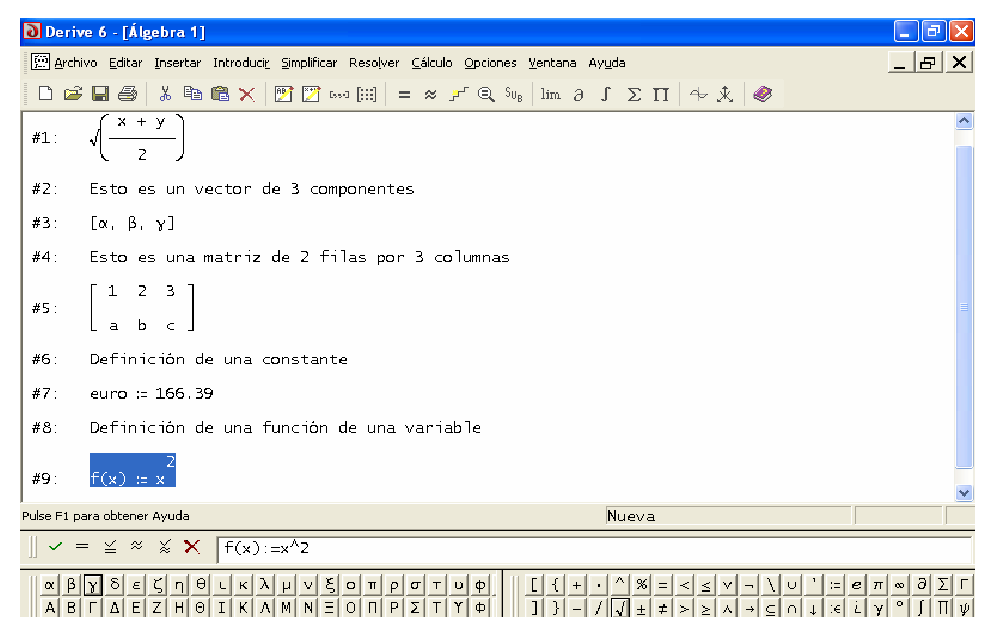
\includegraphics[scale=0.6]{img/introduccion_derive/expresiones}
\caption{Ventana de Algebra con distintos tipos de expresiones.}
\label{g:expresiones}
\end{center}
\end{figure}


\subsection*{Manipulación de archivos}
Las expresiones y los cálculos realizados dentro de la ventana de
Álgebra suelen almacenarse en archivos.

\subsubsection*{Guardar un archivo}
Para crear un archivo donde se guarden las expresiones de la ventana
de Álgebra se utiliza el menú \menu{Archivo>Guardar}, y en el
cuadro de diálogo que aparece se le da nombre al archivo y se
selecciona la carpeta donde queremos guardarlo. Derive le pone
automáticamente la extensión \texttt{*.dfw} a sus archivos. Una vez
creado el archivo, su nombre aparecerá en la barra de título de la
ventana de Derive. Posteriormente, para guardar cambios en una
ventana de Álgebra, bastará con seleccionar de nuevo el menú
\menu{Archivo>Guardar}, de manera que el archivo se actualizará.

\subsubsection*{Recuperar un archivo}
Para recuperar en una ventana de Álgebra el contenido de un archivo
se utiliza el menú \menu{Archivo>Abrir}, y en en cuadro de
diálogo que aparece se selecciona el archivo deseado.
Automáticamente el contenido del archivo aparece en una ventana
nueva de Álgebra.

Otra forma de abrir archivos es mediante el menú
\menu{Archivo>Leer>Math}, que se utiliza para almacenar en
memoria la definición de nuevas funciones, presentes en los archivos
con extensión *.mth, que expanden el potencial de cálculo del núcleo
del programa, el cual queda operativo nada más arrancar Derive. Al
igual que antes aparece un cuadro de diálogo donde debemos
seleccionar el archivo que queremos abrir, sólo que ahora, el
contenido del archivo no aparece en una nueva ventana de Álgebra,
sino que se añade en la ventana de Álgebra activa, a continuación de
las expresiones existentes. Otra forma de proceder con igual
resultado es mediante el menú \menu{Archivo>Leer>Utilidades},
que también permite acceder hasta, y cargar en memoria, los archivos
con extensión *.mth, pero en este caso el conjunto de expresiones
que componen dichos archivos no aparece en la pantalla, aunque sí
que, al estar cargadas en la memoria del ordenador, serán
operativas.

\subsubsection*{Cerrar y abrir nuevas ventanas de Álgebra}
Cuando terminemos una sesión de trabajo, podemos cerrar la ventana
de Álgebra correspondiente mediante el menú
\menu{Archivo>Cerrar}. Por otro lado, en cualquier momento de una
sesión de trabajo podemos abrir, añadidas a la que aparece por
defecto, tantas ventanas de Álgebra como estimemos oportunas
mediante el menú \menu{Archivo>Nuevo}. El programa trabaja con
cada una de las ventanas de Álgebra activas de forma completamente
independiente, lo cual implica, entre otras cosas, que podremos
utilizar los mismos nombres de variables en todas las ventanas
abiertas sin interferencia entre las mismas.

\subsubsection*{Impresión}
Para imprimir el contenido de una ventana de Álgebra, o bien una
gráfica, se utiliza el menú \menu{Archivo>Imprimir}. En el caso
de una ventana de Álgebra aparecerá un cuadro de diálogo donde se
puede seleccionar \texttt{Todo}, para imprimir todo el contenido de
la ventana, \texttt{Páginas} para imprimir un rango de páginas o
\texttt{Selección} para imprimir la zona previamente seleccionada de
la ventana. No obstante, antes de imprimir, conviene utilizar el
menú \menu{Archivo>Vista Previa} para ver por pantalla cómo
quedaría la hoja impresa. Si todo está bien, bastaría con pulsar el
botón \texttt{Imprimir} para que aparezca el cuadro de diálogo de
impresión y desde ahí enviarlo a la impresora. La orientación y los
márgenes pueden cambiarse con el menú \menu{Archivo>Configurar
Página}, mientras que otras opciones como el tipo de letra, o el
encabezado y pie de página se controlan mediante el menú
\menu{Opciones>Impresión>Cabecera y Pie}.

\subsection*{Simplificación de expresiones}
Derive incorpora varios sistemas de simplificación de expresiones.
El más sencillo es la simplificación básica, que puede realizarse
mediante el menú \menu{Simplificar>Normal}. Este menú permite
realizar simplificaciones simples como por ejemplo convertir la
expresión $x+x$ en la expresión $2x$. Sin embargo, no permite pasar
de un binomio como $(x+1)^2$ a su desarrollo $x^2+2x+1$, ya que no
está claro cuál de las dos expresiones es más simple. Para obtener
el desarrollo de este binomio se utiliza el menú
\menu{Simplificar>Expandir} que permite expandir una expresión
con respecto sus variables. Por el contrario, si lo que queremos es
pasar del desarrollo a la forma del binomio, se utiliza el menú
\menu{Simplificar>Factorizar} que permite factorizar una
expresión con respecto a sus variables.

En cualquiera de estas simplificaciones, Derive trabaja por defecto
en modo exacto y por eso devuelve expresiones fraccionarias. Para
obtener el valor de una expresión en modo aproximado, con decimales,
se utiliza el menú \menu{Simplificar>Aproximar}. Con este menú
aparece un cuadro de diálogo donde debemos introducir el número de
decimales que queremos para la aproximación.

Por último, es posible sustituir cualquier variable de una expresión
por un valor u otra expresión mediante el menú
\menu{Simplificar>Sustituir Variable}. En el cuadro de diálogo
que aparece se elige la variable a sustituir y se introduce la
expresión o el valor de sustitución en \texttt{Nuevo Valor}.

\subsection*{Representaciones gráficas}
Derive permite representar gráficamente funciones en 2 y 3
dimensiones.
\subsubsection*{Gráficas en 2 dimensiones}
Para representar una función o expresión de una variable, se
selecciona la expresión y se utiliza el menú \menu{Ventana>Nueva
Ventana 2D}. Automáticamente aparece una ventana de gráficas en 2
dimensiones con unos ejes cartesianos, y para que aparezca la
gráfica de la función, basta con pulsar el menú
\menu{Insertar>Gráfica} de esta ventana, o pulsar en su
correspondiente botón de la barra de botones. En la
figura~\ref{g:2d-plot} se muestra un ejemplo de gráfica en 2
dimensiones.

Si queremos que la gráfica, una vez obtenida, también aparezca en la
ventana de Álgebra como un objeto más de la misma, desde la ventana
2D, utilizamos el menú \menu{Archivo>Incrustar}.

\begin{figure}[h!]
\begin{center}
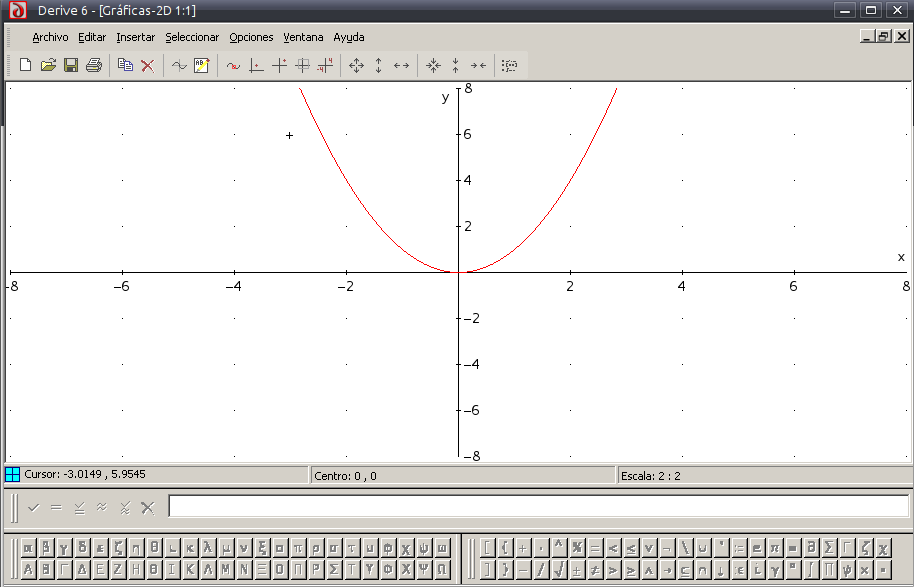
\includegraphics[scale=0.6]{img/introduccion_derive/2d-plot}
\caption{Ventana de gráficas en 2 dimensiones.} \label{g:2d-plot}
\end{center}
\end{figure}

Es posible representar más de una función en una misma gráfica,
seleccionando la nueva expresión en la ventana de Álgebra, y
pulsando de nuevo el menú \menu{Insertar>Gráfica} en la ventana
de gráficos en 2 dimensiones en que queramos que aparezca la
representación gráfica de la expresión seleccionada. Cuando se
quieren representar varias funciones, a veces resulta más cómodo
mostrar al mismo tiempo la ventana de Álgebra y la de gráficas
mediante el menú \menu{Ventana>Mosaico Vertical}, tal y como se
muestra en la figura~\ref{g:expresionesygraficas}.

\begin{figure}[h!]
\begin{center}
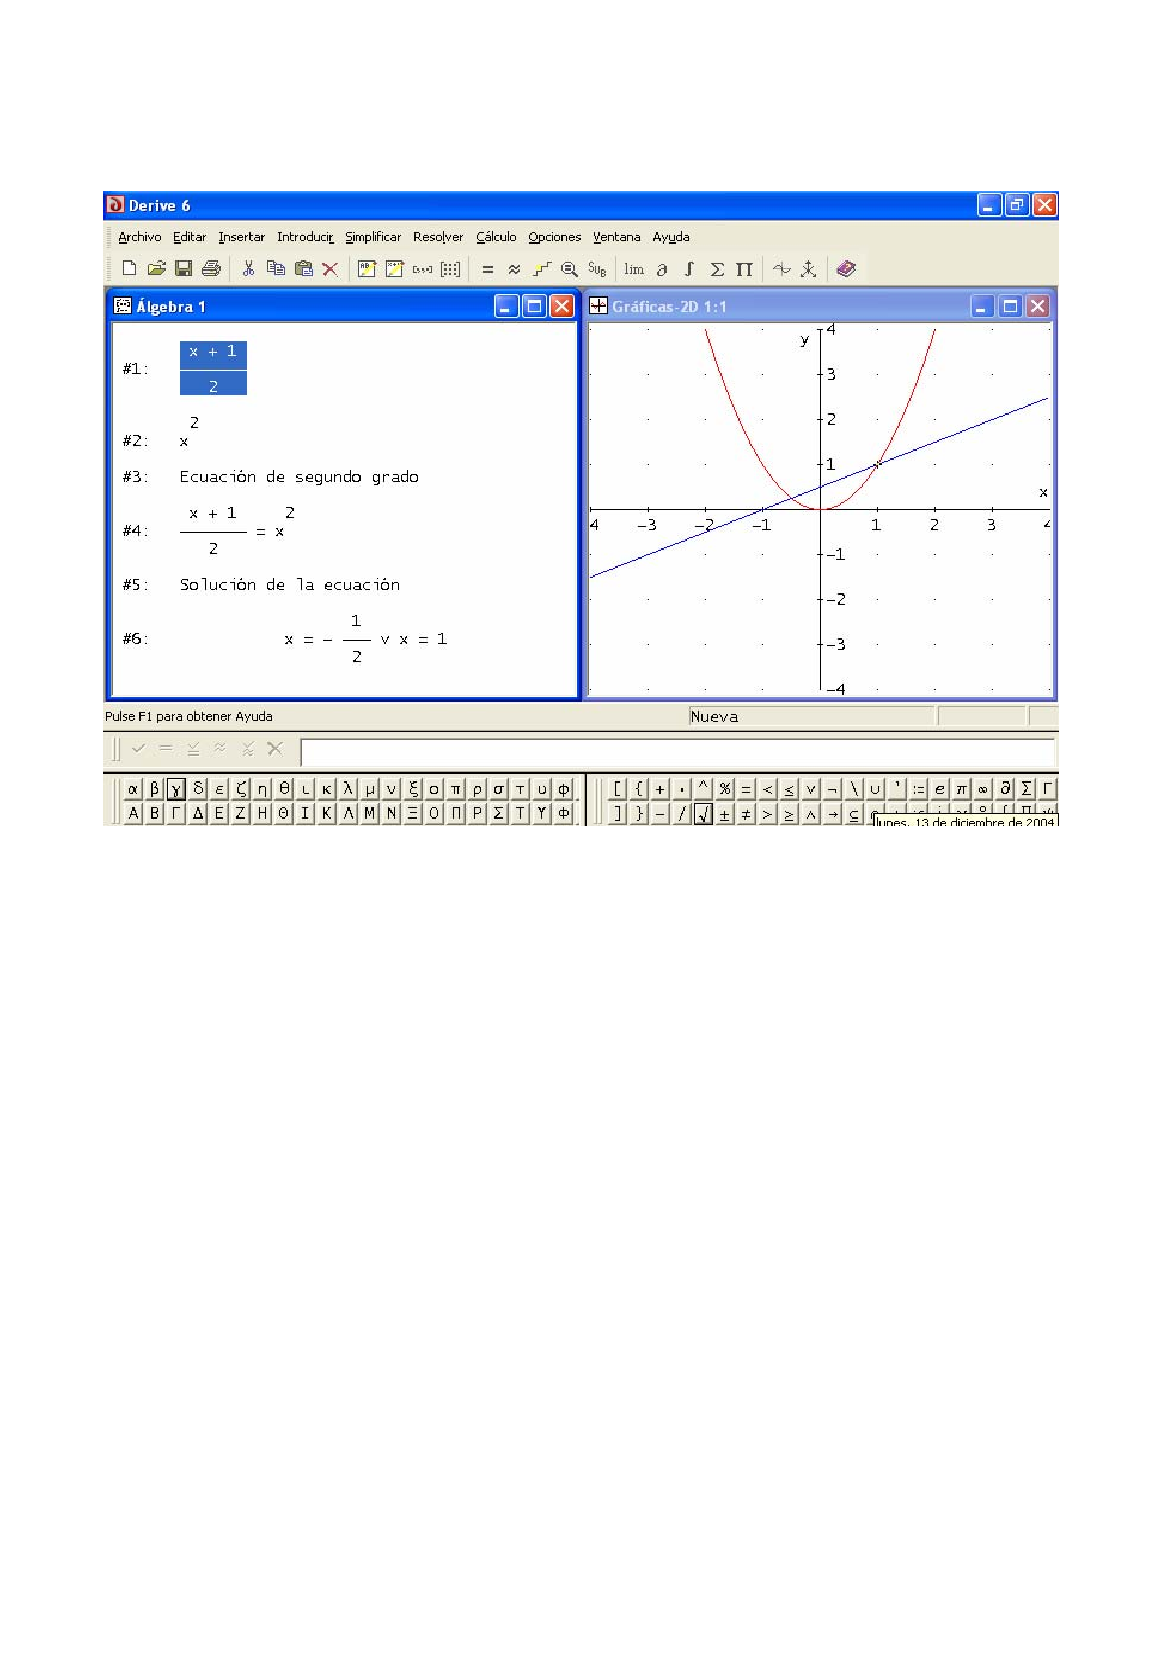
\includegraphics[scale=0.6]{img/introduccion_derive/expresionesygraficas}
\caption{Ventana de Álgebra y de gráficas en 2 dimensiones en una
misma pantalla.} \label{g:expresionesygraficas}
\end{center}
\end{figure}

También es posible borrar gráficas mediante el menú
\menu{Editar>Borrar Gráfica}. Si se elige la opción
\texttt{Primera} se borra la primera gráfica dibujada, si se elige
la opción \texttt{Última} se borra la última, y si se elige la
opción \texttt{Anteriores} borra todas las gráficas excepto la
última.

En la ventana de gráficas en 2 dimensiones existen distintos menús
que permiten cambiar el aspecto de la gráfica representada. Una
posibilidad muy interesante es cambiar la escala de los ejes
mediante el menú \menu{Seleccionar>Relación de Aspecto}.

También es posible ampliar la representación gráfica de una
determinada zona del gráfico mediante el menú
\menu{Seleccionar>Rango de la Gráfica}, introduciendo las
coordenadas de la zona que queremos ampliar, aunque es más práctico
utilizar el botón \texttt{Seleccionar el rango}, y después utilizar
el ratón para delimitar la zona que queremos ampliar.

En la ventana de gráficas en 2 dimensiones aparece una cruz que
representa al cursor. Las coordenadas del cursor siempre aparecen en
la barra de estado. Cuando se pulsa la tecla \texttt{F3}, la cruz se
transforma en un cuadradito y se pasa a \emph{modo de traza}. En
este modo, al mover el cursor con las flechas del teclado, el cursor
sigue la trayectoria de la función representada, con lo que podemos
averiguar los valores que toma la misma en la barra de estado, tal y
como se muestra en la figura~\ref{g:modotraza}.

\begin{figure}[h!]
\begin{center}
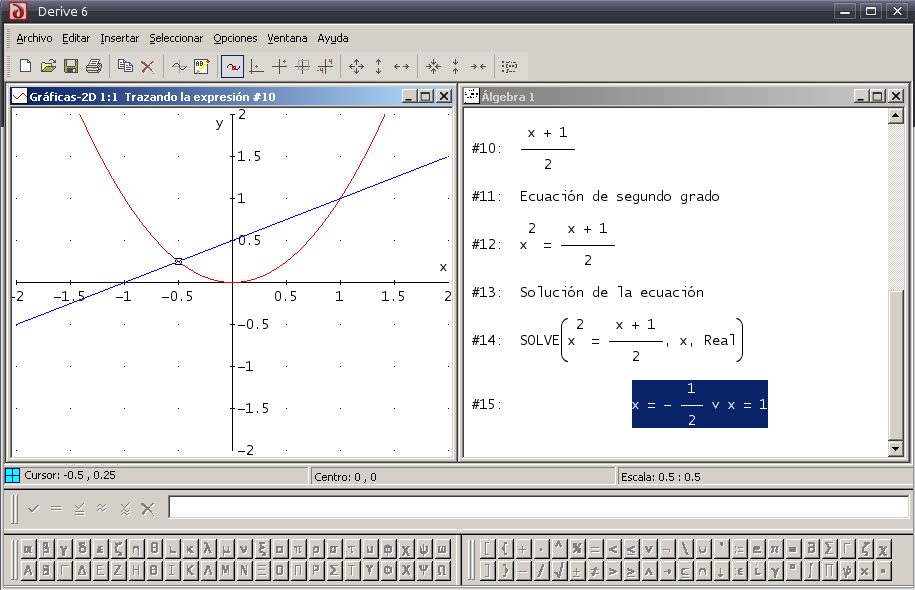
\includegraphics[scale=0.6]{img/introduccion_derive/modotraza}
\caption{Ventana de gráficas en 2 dimensiones en modo de traza con
una gráfica ampliada.} \label{g:modotraza}
\end{center}
\end{figure}

Es posible centrar la gráfica de una función en cualquier punto
mediante el menú \menu{Seleccionar>Rango de la
Gráfica>Longitud/Centro}, aunque, de nuevo, tal vez sea más
operativo hacerlo mediante los botones \texttt{Centrar en el cursor}
y \texttt{Centrar en el origen}.

\subsubsection*{Gráficas en 3 dimensiones}
Para representar una función o expresión de dos variables, se
selecciona la expresión y se utiliza el menú \menu{Ventana>Nueva
Ventana 3D}. Automáticamente aparece una ventana de gráficas en 3
dimensiones con unos ejes cartesianos, y para que aparezca la
gráfica de la función, basta con pulsar el menú
\menu{Insertar>Gráfica} de esta ventana. En la
figura~\ref{g:3d-plot} se muestra un ejemplo de gráfica en 3
dimensiones.

\begin{figure}[h!]
\begin{center}
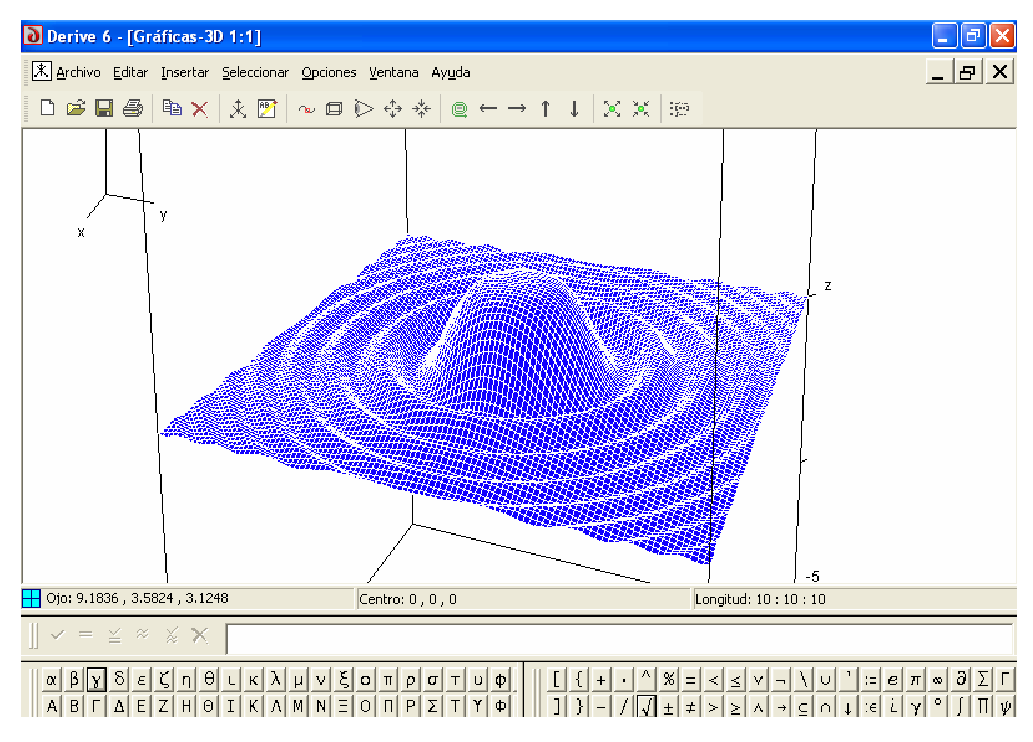
\includegraphics[scale=0.6]{img/introduccion_derive/3d-plot}
\caption{Ventana de gráficas en 3 dimensiones.} \label{g:3d-plot}
\end{center}
\end{figure}

Al igual que en el caso de las gráficas de 2 dimensiones, existen
distintos menús que permiten cambiar el aspecto de la gráfica
representada. De todos ellos, sólo comentaremos el menú
\menu{Editar>Gráfica>Número de Paneles} que permite cambiar la
resolución del gráfico, y el menú \menu{Seleccionar>Posición de
Ojo} que permite cambiar la posición desde donde se mira la gráfica.

 
%$HeadURL: https://practicas-derive.googlecode.com/svn/trunk/funciones_elementales.tex $
%$LastChangedDate: 2009-11-16 16:11:46 +0100 (lun, 16 nov 2009) $
%$LastChangedRevision: 5 $
%$LastChangedBy: asalber $

\chapter{Funciones Elementales}

\section{Fundamentos teóricos}

En esta práctica se introducen los conceptos básicos sobre funciones reales de variable real, esto es, funciones
\[f:\mathbb{R}\rightarrow \mathbb{R}.\]

\subsection{Dominio e imagen}

El \emph{Dominio} de la función $f$ es el conjunto de los números
reales $x$ para los que existe $f(x)$ y se designa mediante $\dom
f$.

La \emph{Imagen} de $f$ es el conjunto de los números reales $y$ para los que existe algún $x\in \mathbb{R}$ tal que $f(x)=y$, y se denota por $\im f$.


\subsection{Signo y crecimiento}
El \emph{signo} de la función es positivo $(+)$ en los valores de $x$ para los que $f(x)>0$ y negativo $(-)$ en los que $f(x)<0$. Los valores de $x$ en los que la función se anula se conocen como \emph{raíces} de la función.

Una función $f(x)$ es \emph{creciente} en un intervalo $I$ si $\forall\, x_1, x_2 \in I$ tales que $x_1<x_2$ se verifica que $f(x_1)\leq f(x_2)$.

Del mismo modo, se dice que una función $f(x)$ es \emph{decreciente} en un intervalo $I$ si $\forall\, x_1, x_2 \in I$ tales que $x_1<x_2$ se verifica que $f(x_1)\geq f(x_2)$. En la figura~\ref{g:crecimiento} se muestran estos conceptos.

\begin{figure}[h!]
\centering \subfigure[Función creciente.] {\label{g:funcion_creciente}
\scalebox{1}{\psset{unit=1.5, ticksize=-3pt 0, algebraic}
\begin{pspicture*}(-1,-0.5)(3,2.5)
\footnotesize
\psaxes[arrows=<->,ticks=none,labels=none](0,0)(-0.5,-0.5)(2.5,2.5)
\psplot[linecolor=blue]{0.5}{1.7}{x^1.5}
\psline[linecolor=red,linestyle=dashed](1,0)(1,1)(0,1)
\psline[linecolor=red,linestyle=dashed](1.5,0)(1.5,1.8371)(0,1.8371)
\psxTick(1){x_1}
\rput[t](1.25,-0.1){$<$}
\psxTick(1.5){x_2}
\psyTick(1){f(x_1)}
\rput[r](-0.3,1.415){\rotateleft{$\leq$}}
\psyTick(1.8371){f(x_2)}
\end{pspicture*} }}\qquad
\subfigure[Función decreciente.]{\label{g:funcion_decreciente}
\scalebox{1}{\psset{unit=1.5, ticksize=-3pt 0, algebraic}
\begin{pspicture*}(-1,-0.5)(3,2.5)
\footnotesize
\psaxes[arrows=<->,ticks=none,labels=none](0,0)(-0.5,-0.5)(2.5,2.5)
\psplot[linecolor=blue]{0.5}{1.7}{2.5-x^1.5}
\psline[linecolor=red,linestyle=dashed](0.8,0)(0.8,1.7845)(0,1.7845)
\psline[linecolor=red,linestyle=dashed](1.3,0)(1.3,1.0178)(0,1.0178)
\psxTick(0.8){x_1}
\rput[t](1.05,-0.1){$<$}
\psxTick(1.3){x_2}
\psyTick(1.7845){f(x_1)}
\rput[r](-0.3,1.415){\rotateleft{$\leq$}}
\psyTick(1.0178){f(x_2)}
\end{pspicture*}}}
\caption{Crecimiento de una función.}
\label{g:crecimiento}
\end{figure}


\subsection{Extremos Relativos}
Una función $f(x)$ tiene un \emph{máximo relativo} en $x_0$ si existe un entorno $A$ de $x_0$ tal que $\forall x \in A$
se verifica que $f(x)\leq f(x_0)$.

Una función $f(x)$ tiene un \emph{mínimo relativo} en $x_0$ si existe un entorno $A$ de $x_0$ tal que $\forall x\in A$
se verifica que $f(x)\geq f(x_0)$.

Diremos que la función $f(x)$ tiene un \emph{extremo relativo} en un punto si tiene un \emph{máximo o mínimo relativo}
en dicho punto. Estos conceptos se muestran en la figura~\ref{g:extremos}.

\begin{figure}[h!]
\centering \subfigure[Máximo relativo.] {\label{g:maximo}
\scalebox{1}{\psset{unit=1.5, ticksize=-3pt 0, algebraic}
\begin{pspicture*}(-1,-0.5)(3.5,2.5)
\footnotesize
\psaxes[arrows=<->,ticks=none,labels=none](0,0)(-0.5,-0.5)(3.5,2.5)
\psplot[linecolor=blue]{0.5}{3.1}{2-(x-1.8)^2}
\psline[linecolor=red,linestyle=dashed](1.8,0)(1.8,2)(0,2)
\psline[linecolor=red,linestyle=dashed](1,0)(1,1.36)(0,1.36)
\psxTick(1.8){x_0}
\psxTick(1){x}
\psxTick(0.5){x_0-\delta}
\psxTick(3.1){x_0+\delta}
\psyTick(2){f(x_0)}
\psyTick(1.36){f(x)}
\rput[r](-0.3,1.72){\rotateleft{$\leq$}}
\psdot[linecolor=green](1.8,2)
\end{pspicture*}}}\qquad
\subfigure[Mínimo relativo.]{\label{g:minimo}
\scalebox{1}{\psset{unit=1.5, ticksize=-3pt 0, algebraic}
\begin{pspicture*}(-1,-0.5)(3.5,2.5)
\footnotesize
\psaxes[arrows=<->,ticks=none,labels=none](0,0)(-0.5,-0.5)(3.5,2.5)
\psplot[linecolor=blue]{0.5}{3.1}{(x-1.8)^2+0.5}
\psline[linecolor=red,linestyle=dashed](1.8,0)(1.8,0.5)(0,0.5)
\psline[linecolor=red,linestyle=dashed](1,0)(1,1.14)(0,1.14)
\psxTick(1.8){x_0}
\psxTick(1){x}
\psxTick(0.5){x_0-\delta}
\psxTick(3.2){x_0+\delta}
\psyTick(0.5){f(x_0)}
\psyTick(1.14){f(x)}
\rput[r](-0.3,0.8){\rotateleft{$\leq$}}
\psdot[linecolor=green](1.8,0.5)
\end{pspicture*}}}
\caption{Extremos relativos de una función.}
\label{g:extremos}
\end{figure}

Una función $f(x)$ está \emph{acotada superiormente} si $\exists K\in\mathbb{R}$ tal que $f(x)\leq K$ $\forall x \in \dom f$. Análogamente, se dice que una función $f(x)$ está \emph{acotada inferiormente} si $\exists K\in\mathbb{R}$ tal que $f(x)\geq K$ $\forall x \in \dom f$.

Una función $f(x)$ está \emph{acotada} si lo está superior e inferiormente, es decir si $\exists K\in\mathbb{R}$ tal que $|f(x)|\leq K$ $\forall x \in \dom f$.


\subsection{Concavidad}

De forma intuitiva se puede decir que una función $f(x)$ es \emph{cóncava} en un intervalo $I$ si $\forall\, x_1, x_2
\in I$, el segmento de extremos $(x_1,f(x_1))$ y $(x_2,f(x_2))$ queda por encima de la gráfica de $f$.

Análogamente se dirá que es \emph{convexa} si el segmento anterior queda por debajo de la gráfica de $f$.

Diremos que la función $f(x)$ tiene un \emph{punto de inflexión} en $x_0$ si en ese punto la función pasa de cóncava a
convexa o de convexa a cóncava. Estos conceptos se ilustran en la figura~\ref{g:concavidad}.

\begin{figure}[h!]
\centering \subfigure[Función cóncava.] {\label{g:funcion_concava_arriba}
\scalebox{1}{\psset{unit=1.5, ticksize=-3pt 0, algebraic}
\begin{pspicture*}(-1,-0.5)(3.5,2.5)
\footnotesize
\psaxes[arrows=<->,ticks=none,labels=none](0,0)(-0.5,-0.5)(3.5,2.5)
\psplot[linecolor=blue]{0.5}{3.1}{(x-1.8)^2+0.5}
\psline[linecolor=red,linestyle=dashed](0.9,0)(0.9,1.31)(0,1.31)
\psline[linecolor=red,linestyle=dashed](2.9,0)(2.9,1.71)(0,1.71)
\psline[linecolor=green,arrows=<->](0.9,1.31)(2.9,1.71)
\psxTick(0.9){x_1}
\psxTick(2.9){x_2}
\psyTick(1.31){f(x_1)}
\psyTick(1.71){f(x_2)}
\end{pspicture*}}}\qquad
\subfigure[Función convexa.]{\label{g:funcion_concava_abajo}
\scalebox{1}{\psset{unit=1.5, ticksize=-3pt 0, algebraic}
\begin{pspicture*}(-1,-0.5)(3.5,2.5)
\footnotesize
\psaxes[arrows=<->,ticks=none,labels=none](0,0)(-0.5,-0.5)(3.5,2.5)
\psplot[linecolor=blue]{0.5}{3.1}{2-(x-1.8)^2}
\psline[linecolor=red,linestyle=dashed](0.9,0)(0.9,1.19)(0,1.19)
\psline[linecolor=red,linestyle=dashed](2.9,0)(2.9,0.79)(0,0.79)
\psline[linecolor=green,arrows=<->](0.9,1.19)(2.9,0.79)
\psxTick(0.9){x_1}
\psxTick(2.9){x_2}
\psyTick(1.19){f(x_1)}
\psyTick(0.79){f(x_2)}
\end{pspicture*}}}
\caption{Concavidad de una función.}
\label{g:concavidad}
\end{figure}

\subsection{Asíntotas}

La recta $x=a$ es una \emph{asíntota vertical} de la función $f(x)$ si al menos uno de los límites laterales de $f(x)$ cuando $x$ tiende hacia $a$ es $+\infty$ o $-\infty$, es decir cuando se verifique alguna de las siguientes igualdades
\[
\ \lim_{x\rightarrow a^{+}}f(x)=\pm\infty   \quad \textrm{o} \quad
\lim_{x\rightarrow a^{-}}f(x)=\pm\infty
\]

La recta $y=b$ es una \emph{asíntota horizontal} de la función $f(x)$ si alguno de los límites de $f(x)$ cuando $x$ tiende hacia $+\infty$ o $-\infty$ es igual a $b$, es decir cuando se verifique
\[
\ \lim_{x\rightarrow -\infty }f(x)=b    \quad \textrm{o} \quad
\ \lim_{x\rightarrow +\infty }f(x)=b
\]

La recta $y=mx+n$ es una \emph{asíntota oblicua} de la función $f(x)$ si alguno de los límites de $f(x)-(mx+n)$ cuando $x$ tiende hacia $+\infty$ o $-\infty$ es igual a 0, es decir si

\[
\ \lim_{x\rightarrow -\infty }{(f(x)-mx)}=n    \quad \textrm{o} \quad
\ \lim_{x\rightarrow +\infty }{(f(x)-mx)}=n
\]

En la figura~\ref{g:asintotas} se muestran los distintos tipos de asíntotas.

\begin{figure}[h!]
\centering \subfigure[Asíntota horizontal y vertical.] {\label{g:asintotahorizontalyvertical}
\scalebox{1}{\psset{unit=0.5,yunit=0.8, algebraic, ticksize=-3pt 0, linewidth=0.8pt}
\begin{pspicture*}(-1,-1)(10,10)
\footnotesize
\psaxes[arrows=<->,ticks=none](0,0)(-1,-1)(10,10)
\psplot[linecolor=blue]{0}{3.8}{1/(x-4)+5}
\psplot[linecolor=blue]{4.1}{10}{1/(x-4)+5}
\psline[linecolor=red](0,5)(10,5)
\psline[linecolor=red](4,0)(4,10)
\psxTick(4){a}
\psyTick(5){b}
\rput[r](10,4.5){Asíntota horizontal}
\rput[r](10,3.5){$y=b$}
\rput[l](4.2,1.5){Asíntota vertical}
\rput[l](4.2,0.5){$x=a$}
\end{pspicture*}


}}\qquad\qquad
\subfigure[Asíntota vertical y oblicua.]{\label{g:asintotaoblicua}
\scalebox{1}{\psset{unit=0.5,yunit=0.8,algebraic, ticksize=-3pt 0,linewidth=0.8pt}
\begin{pspicture*}(-1,-1)(10,10)
\footnotesize
\psaxes[arrows=<->,ticks=none](0,0)(-1,-1)(10,10)
\psplot[linecolor=blue]{0}{3.9}{((x-4)^2+0.5)/(x-4)+5}
\psplot[linecolor=blue]{4.05}{9}{((x-4)^2+0.5)/(x-4)+5}
\psplot[linecolor=red]{0}{9}{x+1}
\psline[linecolor=red](4,0)(4,10)
\psxTick(4){a}
\psyTick(1){b}
\rput[r](10,6){Asíntota oblicua}
\rput[r](10,5){$y=b+cx$}
\rput[l](4.2,1.5){Asíntota vertical}
\rput[l](4.2,0.5){$x=a$}
\end{pspicture*}


}}
\caption{Tipos de asíntotas de una función.}
\label{g:asintotas}
\end{figure}


\subsection{Periodicidad}
Una función $f(x)$ es \emph{periódica} si existe $h\in\mathbb{R^{+}}$ tal que \[f(x+h)=f(x)\  \forall x\in \dom f\] siendo el período $T$ de la función, el menor valor $h$ que verifique la igualdad anterior.

En una función periódica, por ejemplo $f(x)=A\sen(wt)$, se denomina \emph{amplitud} al valor de $A$, y es la mitad de la diferencia entre los valores máximos y mínimos de la función. En la figura~\ref{g:periodoyamplitud} se ilustran estos conceptos.

\begin{figure}[h!]
\centering
\scalebox{1}{\psset{unit=1.5,algebraic}
\begin{pspicture*}(-4,-1.5)(3.5,1.5)
\psaxes[ticks=none,labels=none]{<->}(-1.9634,0)(-2.1,-1.5)(2.1,1.5)
\psplot[linecolor=blue,plotpoints=100]{-1.9634}{2}{cos(4*x)}
\psline[linecolor=red]{|-|}(-1.57075,1)(0,1)
\rput[b](-0.78,1.1){Periodo}
\psline[linecolor=red]{|-|}(0,0)(0,1)
\rput[r](-0.1,0.5){\rotateleft{Amplitud}}
\end{pspicture*}}
\caption{Periodo y amplitud de una función periódica.}
\label{g:periodoyamplitud}
\end{figure}

\clearpage
\newpage

\section{Ejercicios resueltos}

\begin{enumerate}[leftmargin=*]
\item Se considera la función

\[
\ f(t)=\frac{t^{4} +19\cdot t^{2} - 5}{t^{4} +9\cdot t^{2} - 10}.
\]

Representarla gráficamente y determinar a partir de dicha representación:


\begin{enumerate}

\item  Dominio.

\begin{indicacion}
{
\begin{enumerate}

\item Para representarla, podemos definir la función en la línea
de editor (o introducirla directamente, sin generar una
definición), y posteriormente utilizamos el botón \texttt{Ventana
2D} para pasar a la ventana de gráficas 2D, y allí pinchamos en el
botón \texttt{Representar Expresión}).

\item Una vez en la Ventana 2D, y ya que vamos a trabajar con la
gráfica de la función durante todo el ejercicio, probablemente
convenga el Modo de Traza, en el que el cursor se desplaza a lo
largo de la gráfica. Para ello pinchar en el botón \texttt{Trazar
las Gráficas}.

\item Para determinar el dominio tan sólo hay que determinar los
valores de $x$ en los que existe la función.

\item Recordar que, tanto para éste como para el resto de los
apartados del ejercicio, pretendemos llegar a conclusiones
aproximadas que tan sólo sacamos del análisis de la gráfica.

\end{enumerate}

}
\end{indicacion}


\item  Imagen.

\begin{indicacion}
{Fijarse en los valores de la variable $y$ hasta los que llega la
función.}
\end{indicacion}


\item  Asíntotas.

\begin{indicacion}
{Son las líneas rectas, ya sea horizontales, verticales u
oblicuas, hacia las que tiende la función.}
\end{indicacion}

\item  Raíces.



\begin{indicacion}
{Son los valores de la variable $x$, si los hay, en los que la
función vale 0.}

\end{indicacion}

\item  Signo.

\begin{indicacion}
{Hay que determinar, aproximadamente, por un lado los intervalos
de variable $x$ en los que la función es positiva, y por el otro
aquellos en los que es negativa. }
\end{indicacion}

\item  Intervalos de crecimiento y decrecimiento.

\begin{indicacion}
{De nuevo, por un lado hay que determinar los intervalos de
variable $x$ en los que a medida que crece $x$ también lo hace
$y$, que serían los intervalos de crecimiento, y también aquellos
otros en los que a medida que crece $x$ decrece $y$, que serían
los intervalos de decremimiento. }
\end{indicacion}

\item Intervalos de concavidad y convexidad.

\begin{indicacion}
{Para los intervalos de concavidad y convexidad, nos fijamos en el
segmento de línea recta que une dos puntos cualquiera del
intervalo. Si dicho segmento queda por encima de la gráfica,
entonces la función es cóncava en el intervalo, mientras que si
queda por debajo, entonces es convexa en el mismo. }
\end{indicacion}

\item Extremos relativos.

\begin{indicacion}
{Determinamos, aproximadamente, los puntos en los que se
encuentran los máximos y mínimos relativos de la función. }
\end{indicacion}

\item Puntos de inflexión.

\begin{indicacion}
{Determinamos, aproximadamente, los puntos en los que la función
cambia de curvatura, de cóncava a convexa o a la inversa. }
\end{indicacion}

\end{enumerate}



\item Representar en una misma gráfica las funciones $2^{x}, e^{x}, 0.7^{x}, 0.5^{x}$.
\begin{enumerate}
\item A la vista de las gráficas obtenidas, indicar cuáles de las funciones anteriores son crecientes y cuáles son decrecientes.

\begin{indicacion}
{
\begin{enumerate}

\item Aunque podríamos representar en una misma gráfica todas las
funciones dadas a la vez  (sin más que introducir sus expresiones,
marcar todas ellas, irnos a la ventana 2D, y pinchando en el botón
\texttt{Representar Expresiones}), más bien conviene representar
las funciones una a una, y utilizar el botón \texttt{Insertar
Anotación} para asignara a cada una de las gráficas una pequeña
anotación que nos ayude a distinguirla de las demás. Si
desactivamos el modo de trazado y pasamos al modo habitual en el
que podemos situarnos con el cursor en cualquier punto de la
gráfica, podemos trasladar la anotación desde la posición
inicialmente escogida para su ubicación en cualquier otro punto de
la gráfica, sin más que pinchar con el ratón en la anotación, y,
manteniendo pulsado el mismo, arrastrar hasta la nueva ubicación.

\end{enumerate}


}
\end{indicacion}

\item Determinar, a partir de los resultados obtenidos, o representando nuevas funciones si fuera necesario, para qué valores de $a$ será creciente la función $a^{x}$.


\item Determinar, a partir de los resultados obtenidos, o representando nuevas funciones si fuera necesario, para qué valores de $a$ será decreciente la función $a^{x}$.

\begin{indicacion}
{Para los dos apartados anteriores, si no somos capaces de
determinar para qué valores de $a$ la exponencial es creciente o
decreciente, representar en una nueva gráfica las funciones:
$(1,1)^x,1^x$ y $(0,9)^x$.

}
\end{indicacion}

\end{enumerate}




\item Representar en una misma gráfica las funciones siguientes, indicando su período y amplitud.

\begin{enumerate}

\item $\sen{x}$, $\sen{x}+2$, $\sen{(x+2)}$.

\item $\sen{2x}$, $2\sen{x}$, $\sen\frac{x}{2}$.

\begin{indicacion}
{ De nuevo, en ambos apartados conviene representar las funciones
una a una, e incluir anotaciones que nos hagan recordar a qué
función corresponde cada gráfica.


}
\end{indicacion}

\end{enumerate}

\item Representar en una gráfica la función

\[
\ f(x)=\left\{%
\begin{array}{cl}
    -2x & \hbox{si $x\leq0$;} \\
    x^{2} & \hbox{si $x>0$.} \\
\end{array}%
\right.
\]

\begin{indicacion}
{Para representar funciones a trozos, Derive utiliza una función
predefinida llamada $\operatorname{chi}$. La sintaxis de esta
función es $\operatorname{CHI}$ $(a,x,b)$, donde $a$ u $b$ son los
límites de un intervalo, y $x$ es la variable de la función, y se
define cómo:


\[
\operatorname{CHI} (a,x,b) = \left\{ {\begin{array}{*{20}c}
   0 & {\text{si}} & {x < a}  \\
   1 & {\text{si}} & {a \leqslant x \leqslant b}  \\
   0 & {\text{si}} & {x > b}  \\

 \end{array} } \right.
\]


Según esto, para representar la función anterior, habría que
introducir la expresión

\[
-2x \operatorname{CHI}(-inf,x,0)+x^2\operatorname{CHI}(0,x,inf)
\]

\textbf{¡Cuidado!}: a pesar de que la función $\operatorname{CHI}$
es una función interna del programa, y que, por tanto, debería
permitir que se introdujese en mayúsculas o en minúsculas
indistintamente, al intentar introducirla en minúsculas da
errores. Por ello, es conveniente, y puede que incluso
indispensable, introducirla en mayúsculas. }
\end{indicacion}


\end{enumerate}


\section{Ejercicios propuestos}

\begin{enumerate}[leftmargin=*]
\item Hallar el dominio de las siguientes funciones a partir de sus representaciones gráficas:

\begin{enumerate}
\item
$
\ f(x)=\dfrac{x^{2} + x + 1}{x^{3} - x}
$

\item $g(x)=\sqrt[2]{x^{4}-1}$.

\item $h(x)=\cos{\dfrac{x + 3}{x^{2} + 1}}$.
\item $l(x)=\arcsen{\dfrac{x}{1+x}}$.
\end{enumerate}


\item Se considera la función

\[
\ f(x)=\frac{x^{3} + x +2}{5x^{3} - 9x^{2} - 4x + 4}.
\]

Representarla gráficamente y determinar a partir de dicha representación:


\begin{enumerate}
\item  Dominio.
\item  Imagen.
\item  Asíntotas.
\item  Raíces.
\item  Signo.
\item  Intervalos de crecimiento y decrecimiento.
\item  Intervalos de concavidad y convexidad.
\item  Extremos relativos.
\item  Puntos de inflexión.
\end{enumerate}

\item Representar en una misma gráfica las funciones $\log_{10}{x}$, $\log_{2}{x}$, $\log{x}$, $\log_{0.5}{x}$.


\begin{enumerate}

\item A la vista de las gráficas obtenidas, indicar cuáles de las funciones anteriores son crecientes y cuáles son decrecientes.

\item Determinar, a partir de los resultados obtenidos, o representando nuevas funciones si fuera necesario, para qué valores de $a$ será creciente la función $\log_{a}{x}$.

\item Determinar, a partir de los resultados obtenidos, o representando nuevas funciones si fuera necesario, para qué valores de $a$ será decreciente la función $\log_{a}{x}$.


\end{enumerate}

\item Completar las siguientes frases con la palabra igual, o el número de veces que sea mayor o menor en cada caso:

\begin{enumerate}

\item La función $\cos{2x}$ tiene un período............ que la función $\cos{x}$.

\item La función $\cos{2x}$ tiene una amplitud............ que la función $\cos{x}$.

\item La función $\cos\dfrac{x}{2}$ tiene un período............ que la función $\cos{3x}$.

\item La función $\cos\dfrac{x}{2}$ tiene una amplitud............ que la función $\cos{3x}$.

\item La función $3\cos{2x}$ tiene un período............ que la función $\cos\dfrac{x}{2}$.

\item La función $3\cos{2x}$ tiene una amplitud............ que la función $\cos\dfrac{x}{2}$.

\end{enumerate}

\item Hallar a partir de la representación gráfica, las soluciones de $e^{-1/x}=\dfrac{1}{x}$.

\item Representar en una gráfica la función

\[
\ f(x)=\left\{%
\begin{array}{ll}
    x^{3} & \hbox{si $x<0$} \\
    e^{x}-1 & \hbox{si $x\geq0$} \\
\end{array}%
\right.
\]

\end{enumerate}











% Author: Alfredo Sánchez Alberca (asalber@ceu.es)
\chapter{Límites y Continuidad}

\section{Fundamentos teóricos}
En esta práctica se introducen los conceptos de límite y continuidad de una función real, ambos muy relacionados.

\subsection{Límite de una función en un punto}
El concepto de límite está muy relacionado con el de proximidad y tendencia de una serie de valores. De manera informal, diremos que $l\in \mathbb{R}$ es el \emph{límite} de una función $f(x)$ en un punto $a\in \mathbb{R}$, si $f(x)$ tiende o se aproxima cada vez más a $l$, a medida que $x$ se aproxima a $a$, y se escribe
\[ \lim_{x\rightarrow a} f(x)=l.\]

Si lo que nos interesa es la tendencia de $f(x)$ cuando nos aproximamos al punto $a$ sólo por un lado, hablamos de \emph{límites laterales}. Diremos que $l$ es el \emph{límite por la izquierda} de una función $f(x)$ en un punto $a$, si $f(x)$ tiende o se aproxima cada vez más a $l$, a medida que $x$ se aproxima a $a$ por la izquierda, es decir con valores $x<a$, y se denota por
\[ \lim_{x\rightarrow a^-} f(x)=l.\]
Del mismo modo, diremos que $l$ es el \emph{límite por la derecha} de una función $f(x)$ en un punto $a$, si $f(x)$ tiende o se aproxima cada vez más a $l$, a medida que $x$ se aproxima a $a$ por la derecha, es decir con valores $x>a$, y se denota por
\[ \lim_{x\rightarrow a^+} f(x)=l.\]

Por supuesto, para que exista el límite global de la función $f(x)$ en el punto $a$, debe existir tanto el límite por la izquierda, como el límite por la derecha, y ser iguales, es decir
\[
\left.
\begin{array}{l}
\displaystyle \lim_{x\rightarrow a^-} f(x)=l\\
\displaystyle \lim_{x\rightarrow a^+} f(x)=l
\end{array}
\right\}
\Longrightarrow
\lim_{x\rightarrow a} f(x)=l.
\]

\subsection{Álgebra de límites}
Para el cálculo práctico de límites, se utiliza el siguiente
teorema, conocido como Teorema de \emph{Álgebra de Límites}.

Dadas dos funciones $f(x)$ y $g(x)$, tales que $\lim_{x\rightarrow
a}f(x)=l_1$ y $\lim_{x\rightarrow a}g(x)=l_2$, entonces se cumple
que:
\begin{enumerate}
\item $\displaystyle \lim_{x\rightarrow a}(f(x)\pm g(x))=l_1\pm l_2$.
\item $\displaystyle \lim_{x\rightarrow a}(f(x)\cdot g(x))=l_1\cdot l_2$.
\item $\displaystyle \lim_{x\rightarrow a}\dfrac{f(x)}{g(x)}=\dfrac{l_1}{l_2}$ si $l_2\neq 0$.
\end{enumerate}

\subsection{Asíntotas}
Como interpretación geométrica de los límites, definiremos rectas
particulares a las que tiende (se ``pega") la gráfica de una función
cuando la variable tiende a un cierto valor, finito o infinito.
\subsubsection*{Asíntotas verticales}
La recta $x=a$ es una \emph{Asíntota Vertical} de la función $f(x)$
si al menos uno de los límites laterales de $f$ en $a$ es $+\infty$
ó $+\infty$. Es decir:

\[
\mathop {\lim }\limits_{x \to a} f(x) =  \pm \infty
\]

\subsubsection*{Asíntotas Horizontales}
La recta $y=b$ es una \emph{Asíntota Horizontal} de la función
$f(x)$ si se cumple:
\[
\mathop {\lim }\limits_{x \to  + \infty } f(x) = b\quad
\text{ó}\quad\mathop {\lim }\limits_{x \to  - \infty } f(x) = b
\]


\subsubsection*{Asíntotas Oblicuas}

La recta $y=mx+n$, donde $m\neq0$, es \emph{Asíntota Oblicua} de la
función $f(x)$ si:


\[
\mathop {\lim }\limits_{x \to  + \infty } \left[ {f(x) - \left( {mx
+ n} \right)} \right] = 0\quad\text{ó}\quad\mathop {\lim }\limits_{x
\to - \infty } \left[ {f(x) - \left( {mx + n} \right)} \right] = 0
\]


La determinación práctica de $m$ y $n$ se realiza del siguiente
modo:

\[
m = \mathop {\lim }\limits_{x \to  + \infty } \frac{{f(x)}} {x}
\]

\[
n = \mathop {\lim }\limits_{x \to  + \infty } \left[ {f(x) - mx}
\right]
\]
o bien lo mismo con los límites en $-\infty$:
\[
m = \mathop {\lim }\limits_{x \to  - \infty } \frac{{f(x)}} {x}
\]

\[
n = \mathop {\lim }\limits_{x \to  - \infty } \left[ {f(x) - mx}
\right]
\]

En cualquiera de los casos, si obtenemos un valor real para $m$ (no
puede ser ni $+\infty$ ni $-\infty$) distinto de $0$, procedemos
después a calcular $n$, que también debe ser real (sí que puede ser
$0$).

Si $m=\pm\infty$ entonces la función crece (decrece) más deprisa que
cualquier recta, y si $m=0$ la función crece (decrece) más despacio
que cualquier recta, y en cualquiera de los dos casos decimos que la
función tiene una \emph{Rama Parabólica}.

\subsection{Continuidad de una función en un punto}
Diremos que una función $f(x)$ es continua en un punto $a\in
\mathbb{R}$, si se cumple
\[ \lim_{x\rightarrow a}f(x)=f(a),\]
donde $f(a)\in \mathbb{R}$.

La definición anterior implica a su vez que se cumplan estas tres
condiciones:

\begin{itemize}

\item Existe el límite de $f$ en $x=a$.

\item La función está definida en $x=a$; es decir, existe $f(a)$.

\item Los dos valores anteriores coinciden.

\end{itemize}

Si la función $f$ no es continua en $x=a$, diremos que es
\emph{discontinua} en el punto $a$, o bien que $f$ tiene una
\emph{discontinuidad} en $a$.

Intuitivamente, una función es continua cuando puede dibujarse su
gráfica sin levantar el lápiz.

\subsubsection*{Continuidad lateral en un punto}

Si nos restringimos a los valores que toma una función a la derecha
de un punto $x=a$, o a la izquierda, se habla de continuidad por la
derecha o por la izquierda según la siguiente definición.

Una función es \emph{continua por la derecha} en un punto $x=a$, y
lo notaremos como $f$ continua en $a^+$, si existe el límite por la
derecha en dicho punto y coincide con el valor de la función en el
mismo:
\[
\mathop {\lim }\limits_{x \to a^ +  } f\left( x \right) = f\left( a
\right)
\]

De igual manera, la función es \emph{continua por la izquierda} en
un punto $x=a$, y lo notaremos como $f$ continua en $a^-$, si existe
el límite por la izquierda en dicho punto y coincide con el valor de
la función en el mismo:

\[
\mathop {\lim }\limits_{x \to a^ -  } f\left( x \right) = f\left( a
\right)
\]


\subsubsection*{Propiedades de la continuidad en un punto}

Como consecuencia de la definición de continuidad en un punto,
podrían demostrarse toda una serie de teoremas, algunos de ellos
especialmente importantes.

\begin{itemize}

\item \textbf{Álgebra de funciones continuas}.
Si $f$ y $g$ son funciones continuas en $x=a$, entonces $f\pm g$ y
$f\cdot g$ son también continuas en $x=a$. Si además $g(a)\neq 0$,
entonces $f/g$ también es continua en $x=a$.

\item \textbf{Continuidad de funciones compuestas}. Si $f$ es continua en
$x=a$ y $g$ es continua en $b=f(a)$, entonces la función compuesta
$g\circ f$ es continua en $x=a$.

\item \textbf{Continuidad y cálculo de límites}. Sean $f$ y $g$ dos
funciones tales que existe $\mathop {\lim }\limits_{x \to a} f(x) =
l$ $\in \mathbb{R}$ y $g$ es una función continua en $l$. Entonces:

\[
\mathop {\lim }\limits_{x \to a} g\left( {f\left( x \right)} \right)
= g\left( l \right)
\]

\end{itemize}

\subsubsection*{Tipos de discontinuidades}
Puesto que la condición de continuidad puede no satisfacerse por
distintos motivos, existen distintos tipos de discontinuidades:


\begin{itemize}
\item \textbf{Discontinuidad evitable}. Se dice que $f(x)$ tiene una \emph{discontinuidad evitable} en el punto $a$, si existe el límite de la función  pero no coincide con el valor de la función en el punto (bien porque sea diferente, bien por que la función no esté definida en dicho punto), es decir
\[\lim_{x\rightarrow a}f(x)=l\neq f(a).\]

\item \textbf{Discontinuidad de salto}. Se dice que $f(x)$ tiene una \emph{discontinuidad de salto} en el punto $a$, si existe el límite de la función por la izquierda  y por la derecha pero son diferentes, es decir,
\[
\lim_{x\rightarrow a^-}f(x)=l_1\neq l_2=\lim_{x\rightarrow a^+}f(x).
\]
A la diferencia entre ambos límites $l_1-l_2$, se le llama
\emph{amplitud del salto}.

\item \textbf{Discontinuidad esencial}. Se dice que $f(x)$ tiene una \emph{discontinuidad esencial} en el punto $a$, si no existe alguno de los límites laterales de la función.
\end{itemize}

\newpage

\section{Ejercicios resueltos}
\begin{enumerate}[leftmargin=*]
\item  Dada la función
\[
f(x)=\left( 1+\frac 2x\right) ^{x/2},
\]
se pide:

\begin{enumerate}
\item  Dibujar su gráfica, y a la vista de misma conjeturar el resultado de los siguientes límites:
\begin{multicols}{2}
\begin{enumerate}
\item  $\lim\limits_{x\rightarrow -\,\infty }\ f(x)$
\item  $\lim\limits_{x\rightarrow +\,\infty }\ f(x)$
\item  $\lim\limits_{x\rightarrow -\,2^{-}}\ f(x)$
\item  $\lim\limits_{x\rightarrow -\,2^{+}}\ f(x)$
\item  $\lim\limits_{x\rightarrow 2}\ f(x)$
\item  $\lim\limits_{x\rightarrow 0}\ f(x)$
\end{enumerate}
\end{multicols}

\begin{indicacion}
\begin{enumerate}
\item Para representar la gráfica de la función, introducir su expresión, acceder a la ventana 2D, y pinchar en el botón \boton{Representar
Expresión}. Probablemente haya que cambiar la escala de la representación original pinchando en el botón de \boton{Zoom hacia fuera en ambos
ejes}, para tener una perspectiva más amplia de la forma de la función.
\item Para predecir cuáles pueden ser los valores de los límites pedidos, observar hacia qué valores tiende la función cuando la variable
$x$ se acerca al valor que aparece en cada límite. Para ello, puede resultar conveniente pinchar en el botón \boton{Trazar gráficas}, para
que el cursor sólo pueda desplazarse a lo largo de la misma.
\end{enumerate}
\end{indicacion}

\item  Calcular los límites anteriores. ¿Coinciden los resultados con los conjeturados?.
\begin{indicacion}
\begin{enumerate}
\item Utilizar el menú \menu{Cálculo > Límites}, o su correspondiente botón de la barra de botones.

\item En el cuadro de diálogo que aparece, seleccionar tanto la variable del límite como el punto en el que queremos calcularlo, y la
tendencia (izquierda, derecha, o ambas).
\end{enumerate}
\end{indicacion}
\end{enumerate}


\item Dada la función 
\[
f(x)=
\begin{cases}
\dfrac{x}{x-2} & \mbox{si $x\leq 0$;}\\
\dfrac{x^2}{2x-6} & \mbox{si $x>0$;}
\end{cases}
\]
\begin{enumerate}
\item Dibujar la gráfica de $f$ y determinar gráficamente si existen asíntotas.
\begin{indicacion}
\begin{enumerate}
\item Introducir la expresión \comando{f(x) := x/(x-2) CHI(-inf,x,0) + x\^{}2/(2x-6) CHI(0,x,inf)} en la ventana de Álgebra y seleccionarla.
\item Abrir una nueva ventana de gráficos en 2D con el menú \menu{Ventana > Nueva Ventana 2D} y selccionar el menú \menu{Ventana -> Mosaico Vertical} para ver la ventana de Álgebra y la de gráficos al mismo tiempo.  
\item Hacer clic en el botón \boton{Representar Expresión} en la ventana gráfica.
\end{enumerate}
\end{indicacion}

\item Calcular las asíntotas verticales de $f$.
\begin{indicacion}
El único punto donde la función no está definida es $x=3$.
Para ver si existe asíntota vertical en ese punto hay que calcular el límite en el punto.
\begin{enumerate}
\item Seleccionar el nombre de la función en la ventana de Álgebra.
\item Seleccionar el menú \menu{Cálculo > Limites} o hacer clic en el botón \boton{Límites}.
\item En el cuadro de diálogo que aparece introducir 3 en el campo \campo{Punto}, seleccionar la opción \opcion{Izquierda} en la lista \campo{Tendiendo por} y hacer clic en el botón \boton{Simplificar}. 
\item Repetir los tres pasos anteriores pero seleccionando la opción \opcion{Derecha} en la lista \campo{Tendiendo por}.
\item Comprobar si el resultado tiene sentido mirando la gráfica.
\end{enumerate}
Existe una asíntota vertical en $x=3$ si alguno de los límites es infinito.
En tal caso, introducir la expresión de la asíntota en la ventana de Álgebra y hacer clic en el botón \boton{Representar expresión} de la ventana gráfica.
\end{indicacion}

\item Calcular las asíntotas horizontales de $f$.
\begin{indicacion}
Para ver si existen asíntotas horizontales hay que calcular los límites en infinito.
\begin{enumerate}
\item Seleccionar el nombre de la función en la ventana de Álgebra.
\item Seleccionar el menú \menu{Cálculo > Limites} o hacer clic en el botón \boton{Limite}.
\item En el cuadro de diálogo que aparece introducir \comando{-inf} en el campo \campo{Punto} y hacer clic en el \boton{Simplificar}. 
\item Repetir los tres pasos anteriores pero introduciendo \comando{inf} en el campo \campo{Punto}.
\item Comprobar si el resultado tiene sentido mirando la gráfica.
\end{enumerate}
Existe una asíntota horizontal $y=a$ si alguno de los límites es $a$.
En tal caso, introducir la expresión de la asíntota en la ventana de Álgebra y hacer clic en el botón \boton{Representar expresión} de la ventana gráfica.
\end{indicacion}

\item Calcular las asíntotas oblicuas de $f$.
\begin{indicacion}
Para ver si existen asíntotas oblicuas hay que calcular el límite en infinito de la función divida por $x$.
Para ver si existe asíntota oblicua en $-\infty$, seguir los pasos siguientes:
\begin{enumerate}
\item Introducir la expresión \comando{f(x)/x} en la ventana de Álgebra y seleccionarla.
\item Seleccionar el menú \menu{Cálculo > Limites} o hacer clic en el botón \boton{Limite}.
\item En el cuadro de diálogo que aparece introducir \comando{-inf} en el campo \campo{Punto} y hacer clic en el \boton{Simplificar}. 
\end{enumerate}
Existe asíntota oblicua $y=ax+b$ si el resultado del límite es $a$.
En tal caso $a$ es la pendiente de la asíntota. 
Para obtener el término independiente hay que calcular el límite en infinito de la función menos $ax$.
\begin{enumerate}
\item Introducir la expresión \comando{f(x)-ax}, donde \comando{a} es el valor del límite anterior, en la ventana de Álgebra y seleccionarla.
\item Seleccionar el menú \menu{Cálculo > Limites} o hacer clic en el botón \boton{Limite}.
\item En el cuadro de diálogo que aparece introducir \comando{-inf} en el campo \campo{Punto} y hacer clic en el \boton{Simplificar}. 
\end{enumerate}
El término independiente de la asíntota oblicua es el resultado del límite. 

Para ver si hay asíntota oblicua en $\infty$ repetir todos los pasos pero introduciendo \comando{inf} en el campo \campo{Punto}.
 
Si existe alguna asíntota oblicua introducir la expresión de la asíntota en la ventana de Álgebra y hacer clic en el botón \boton{Representar expresión} de la ventana gráfica.
\end{indicacion}
\end{enumerate}

\item  Clasificar las discontinuidades de las siguientes funciones en los puntos que se indica.
\begin{multicols}{2}
\begin{enumerate}
\item  $f(x)=\dfrac{\sen x}{x}$ en $x=0$.
\item $g(x)=\dfrac{1}{2^{1/x}}$ en $x=0$.
\item $h(x)=\dfrac{1}{1+e^{\frac{1}{1-x}}}$ en $x=1$.
\end{enumerate}
\end{multicols}

\begin{indicacion}
Para clasificar las discontinuidades en los puntos que se indican, además de definir cada una de las funciones, conviene representar su
gráfica, lo cual, aunque no sirve para demostrar la presencia de una discontinuidad, sí que nos puede dar una idea sobre las
discontinuidades presentes y su tipo (las discontinuidades evitables apenas aparecen visibles en la gráfica, aunque sí que Derive deja un
pequeño hueco en la misma):
\begin{enumerate}
\item Calcular el valor del límite en el punto. Para ello, se puede utilizar el botón \boton{Calcular un límite} de la barra de botones, y
activar la tendencia por \opcion{Ambas} en el cuadro de diálogo que aparece. Si dicho límite existe, entonces la discontinuidad es evitable.
\item Si el límite no existe, puede que sí que existan los laterales. Para calcularlos utilizar el botón \boton{Calcular un límite} y
activar la tendencia por la \opcion{Izquierda} y luego por la \opcion{Derecha}. Si ambos límites laterales existen pero no son iguales, la
discontinuidad será de salto.
\item Si alguno de los límites laterales no existe, entonces la discontinuidad es esencial.
\end{enumerate}
\end{indicacion}


\item  Hallar los puntos de discontinuidad y estudiar el carácter
de dichas discontinuidades en la función:
\[
f(x)=
\left\{
\begin{array}{ll}
\dfrac{x+1}{x^2-1}, & \hbox{si $x<0$;} \\
\dfrac{1}{e^{1/(x^2-1)}}, & \hbox{si $x\geq 0$.} \\
\end{array}
\right.
\]

\begin{indicacion}
\begin{enumerate}
\item Para delimitar los posibles puntos de discontinuidad, previamente definir la función teniendo en cuenta que se trata de una función
definida a trozos. Por lo tanto, habrá que multiplicar el primer tramo por \comando{CHI}$(\infty,x,0)$, y el segundo por
\comando{CHI}$(0,x,\infty)$.
\item Aunque no sirve para demostrar la presencia o no de una discontinuidad, si representamos la gráfica de la función podemos darnos una
idea sobre los puntos en los que aparecen las discontinuidades, teniendo muy presente que las discontinuidades evitables apenas resultan
visibles en la gráfica, aunque sí que Derive deja un pequeño hueco en la misma.
\item Una vez definida la función, hay que encontrar los puntos que quedan fuera del dominio de cada uno de los tramos. Para ello, hay que
analizar dónde se anulan los denominadores presentes en las definiciones de ambos tramos. Por ejemplo, si $x<0$, el denominador $x^2-1$ se
anula en $x=\pm1$; sin embargo tan sólo nos interesa $x=-1$ ya que la definición impone que $x<0$.
\item Cuando ya hemos descubierto cuáles son los puntos que están fuera del dominio, y por tanto son discontinuidades de la función, hay que
analizar cual es su tipo. Para ello, aplicamos el mismo proceso que en el ejercicio anterior (vemos si existe el límite, con lo cual sería
discontinuidad evitable, y si no existe analizamos los laterales para ver si es discontinuidad de salto; si no existe alguno de los
laterales es discontinuidad esencial).
\item Por último, también hay que analizar los puntos en los que hay un cambio de definición de la función. En nuestro caso, en $x=0$, y, de
nuevo, analizando el límite general y los límites laterales.
\end{enumerate}
\end{indicacion}

\end{enumerate}


\section{Ejercicios propuestos}
\begin{enumerate}[leftmargin=*]
\item  Calcular los siguientes límites si existen:
\begin{multicols}{2}
\begin{enumerate}
\item  $\displaystyle \lim_{x\rightarrow 1}\dfrac{x^3-3x+2}{x^4-4x+3}$.
\item  $\displaystyle \lim_{x\rightarrow a}\dfrac{\sen x-\sen a}{x-a}$.
\item $\displaystyle \lim_{x\rightarrow\infty}\dfrac{x^2-3x+2}{e^{2x}}$.
\item $\displaystyle \lim_{x\rightarrow\infty}\dfrac{\log(x^2-1)}{x+2}$.
\item $\displaystyle \lim_{x\rightarrow 1}\dfrac{\log(1/x)}{\tg(x+\dfrac{\pi}{2})}$.
\item $\displaystyle \lim_{x\rightarrow a}\dfrac{x^n-a^n}{x-a}\quad n\in \mathbb{N}$.
\item $ \displaystyle \lim_{x\rightarrow 1}\dfrac{\sqrt[n]{x}-1}{\sqrt[m]{x}-1}\quad n,m \in \mathbb{Z}$.
\item $\displaystyle \lim_{x\rightarrow 0}\dfrac{\tg x-\sen x}{x^3}$.
\item $\displaystyle \lim_{x\rightarrow \pi/4}\dfrac{\sen x-\cos x}{1-\tg x}$.
\item $\displaystyle \lim_{x\rightarrow 0}x^2e^{1/x^2}$.
\item $\displaystyle \lim_{x\rightarrow \infty}\left(1+\dfrac{a}{x}\right)^x$.
\item $\displaystyle \lim_{x\rightarrow \infty} \sqrt[x]{x^2}$.
\item $\displaystyle \lim_{x\rightarrow 0}\left(\dfrac{1}{x}\right)^{\tg x}$.
\item $\displaystyle \lim_{x\rightarrow 0}(\cos x)^{1/\mbox{\footnotesize sen}\, x}$.
\item $\displaystyle \lim_{x\rightarrow 0}\dfrac{6}{4+e^{-1/x}}$.
\item $\displaystyle \lim_{x\rightarrow \infty}\left(\sqrt{x^2+x+1}-\sqrt{x^2-2x-1}\right)$.
\item $\displaystyle \lim_{x\rightarrow \pi/2}\sec x-\tg x$.
\end{enumerate}
\end{multicols}

\item Dada la función:
\[
\renewcommand{\arraystretch}{2}
f(x) = \left\{
\begin{array}{*{20}c}{
\dfrac{{x^2  + 1}}{{x + 3}}} & {\text{si}\;x < 0}  \\
{\dfrac{1}{{e^{1/(x^2  - 1)} }}} & {\text{si}\;x \geqslant 0\;}  \\
\end{array} 
\right.
\]
Calcular todas sus asíntotas.

\item  Las siguientes funciones no están definidas en $x=0$.
Determinar, cuando sea posible, su valor en dicho punto de modo que sean continuas.
\begin{multicols}{2}
\begin{enumerate}
\item  $f(x)=\dfrac{(1+x)^n-1}{x}$.
\item  $h(x)=\dfrac{e^x-e^{-x}}{x}$.
\item  $j(x)=\dfrac{\log(1+x)-\log(1-x)}{x}$.
\item  $k(x)=x^2\sen\dfrac{1}{x}$.
\end{enumerate}
\end{multicols}

\end{enumerate}

\chapter{Derivadas de funciones de una variable}

\section{Fundamentos teóricos}
El concepto de derivada es uno de los más importantes del Cálculo
pues resulta de gran utilidad en el estudio de funciones y tiene
multitud de aplicaciones. En esta práctica introducimos este
concepto y presentamos algunas de sus aplicaciones, tanto en
funciones de una como de varias variables.

\subsection{Tasas de variación media e instantánea. La derivada}
Cuando queremos conocer la variación que experimenta una función
real $f(x)$ en un intervalo $[a,b]$, se calcula la diferencia
$f(b)-f(a)$ que se conoce como \emph{incremento} de $f$, y se nota
$\Delta f[a,b]$, aunque, a veces, simplemente se escribe $\Delta f$.

En muchas otras ocasiones veces resulta importante comparar la
variación que experimenta la función $f$ con relación a la variación
que experimenta su argumento $x$ en un intervalo $[a,b]$. Si tenemos
en cuenta que $b=a+\Delta x$, esto viene dado por la \emph{tasa de
variación media}, que se define como:

\[
\textrm{TVM} f[a,b]=\textrm{TVM} f[a,a+\Delta x]=\frac{\Delta
f}{\Delta x}=\frac{f(b)-f(a)}{b-a}=\frac{f(a+\Delta x )-f(a)}{\Delta
x}.
\]

También resulta muy común llamar a $\Delta x$ con la letra $h$, por
lo que la expresión anterior queda de la forma:

\[
\textrm{TVM} f[a,b]=\textrm{TVM} f[a,a+h]=\frac{\Delta f}{\Delta
x}=\frac{f(a+h)-f(a)}{h}.
\]

Desde el punto de vista geométrico, la tasa de variación media de
$f$ en el intervalo $[a , a+\Delta x]$ es la pendiente de la recta
secante a $f$ en los puntos $(a , f(a))$ y $(a+\Delta x, f(a+\Delta
x))$, tal y como se muestra en la figura~\ref{g:secante}.

\begin{figure}[h!]
\begin{center}
\scalebox{1}{\psset{unit=1.2,xunit=2, ticksize=-3pt 0, algebraic}
\begin{pspicture*}(-1,-0.5)(3.5,4)
\footnotesize
\psaxes[arrows=<->,ticks=none](0,0)(-0.3,-0.3)(2.5,4)
\psplot[linecolor=blue]{0.2}{1.8}{x^3-x^2+x+0.5}
\rput[r](1.4,3.5){$f(x)$}
\psxTick(0.5){a}
\psxTick(1.5){a+\Delta x}
\psline[linewidth=0.5pt,linestyle=dashed,linecolor=gray](0.5,0)(0.5,0.875)
\psline[linewidth=0.5pt,linestyle=dashed,linecolor=gray](1.5,0.875)(0,0.875)
\psline[linewidth=0.5pt,linestyle=dashed,linecolor=gray](1.5,0)(1.5,3.125)(0,3.125)
\psyTick(0.875){f(a)}
\psyTick(3.125){f(a+\Delta x}
\psplot[linecolor=red]{0.2}{1.8}{2.25*x-0.25}
\psline[arrows=|*-|*,linecolor=green](1.5,3.125)(1.5,0.875)
\psline[arrows=|*-|*,linecolor=green](0.5,0.875)(1.5,0.875)
\rput[l](1.6,2){$\Delta y=f(a+\Delta x)-f(a)$}
\rput[t](1,0.8){$\Delta x$}
\end{pspicture*}}
\caption{La tasa de variación media como la pendiente de la recta
secante a una función en dos puntos.} \label{g:secante}
\end{center}
\end{figure}


Y, a veces, incluso más importante que la tasa de variación media,
es estudiar la tasa de variación que experimenta la función, no en
un intervalo, sino en un punto, tomando para ello límites cuando el
incremento en la variable independiente tiende 0. Definimos la tasa
de variación de una función en un punto $a$, o también tasa de
variación instantánea, a partir de la tasa de variación media de la
función en el intervalo $[a,a+\Delta x]$. Dicha tasa, si existe,
recibe el nombre de \emph{derivada} de la función real $f(x)$ en un
punto $a\in \mathbb{R}$, y se nota como $f'(a)$, o bien
$\dfrac{df}{dx}(a)$:

\[
f'(a)=\dfrac{df}{dx}(a)= \lim_{\Delta x\rightarrow 0}\frac{\Delta
f}{\Delta x}=\lim_{\Delta x\rightarrow 0}\frac{f(a+\Delta
x)-f(a)}{\Delta x}=\lim_{h\rightarrow 0}\frac{f(a+h)-f(a)}{h}.
\]

Cuando este límite existe, se dice que la función $f$ es
\emph{derivable} o \emph{diferenciable} en el punto $a$.

Geométricamente, $f'(a)$ es la pendiente de la recta tangente a la
curva de $f(x)$ en el punto $(a,f(a))$, tal y como se aprecia en la
figura~\ref{g:tangente}.

\begin{figure}[h!]
\begin{center}
\scalebox{1}{\psset{unit=1.2,xunit=2, ticksize=-3pt 0, algebraic}
\begin{pspicture*}(-1.5,-0.5)(3,4.5)
\footnotesize
\psaxes[arrows=<->,ticks=none,labels=none](0,0)(-0.3,-0.5)(2,3.5)
\psplot[linecolor=blue]{0.2}{1.5}{x^3-x^2+x+0.5}
\rput[r](1.4,3.5){$f(x)$}
\psxTick(0.5){a}
\psxTick(1.5){x}
\psline[linewidth=0.5pt,linestyle=dashed,linecolor=gray](0.5,0)(0.5,0.875)
\psline[linewidth=0.5pt,linestyle=dashed,linecolor=gray](1.5,0.875)(0,0.875)
\psline[linewidth=0.5pt,linestyle=dashed,linecolor=gray](1.5,0)(1.5,1.625)(0,1.625)
\psyTick(0.875){f(a)}
\psyTick(1.625){f(a)+f'(a)(x-a)}
\psplot[linecolor=red]{0.2}{1.8}{0.75*x+0.5}
\psline[arrows=|*-|*,linecolor=green](1.5,1.625)(1.5,0.875)
\psline[arrows=|*-|*,linecolor=green](0.5,0.875)(1.5,0.875)
\rput[l](1.6,1.25){$f'(a)(x-a)$}
\rput[t](1,0.8){$(x-a)$}
\end{pspicture*}}
\caption{La derivada como la pendiente de la recta tangente a una
función en un punto.} \label{g:tangente}
\end{center}
\end{figure}

\subsubsection*{Recta tangente y normal a una función en un punto}
De la gráfica anterior, fácilmente se deduce que la ecuación de la
recta tangente a una función $f(x)$ en el punto $(a,f(a))$ es:
\[
y=f(a)+f'(a)(x-a).
\]

Y teniendo en cuenta que la pendiente de la recta normal (recta
perpendicular a la recta tangente) es la inversa cambiada de signo,
la ecuación de la recta normal a $f(x)$ en el punto $(a,f(a))$ es:
\[
y=f(a)-\frac{1}{f'(a)}(x-a).
\]

\subsection{Función derivada y derivadas sucesivas}

El límite que nos sirve para calcular la derivada de una función en
un punto, define una nueva función $f'$ cuyo dominio está formado
por los puntos en los que $f$ es diferenciable. La función $f'(x)$,
o también $\dfrac{df}{dx}$, se llama \emph{primera derivada} de $f$.

Puesto que $f'$ es una función, puede derivarse a su vez, y la
primera derivada de $f'$ se conoce como segunda derivada de $f$, y
se nota $f''(x)$ o $\dfrac{d^2f}{dx^2}$. Análogamente, la
\emph{$n$-ésima derivada} de $f$, designada por $f^{(n}$ o
$\dfrac{d^nf}{dx^n}$, es la primera derivada de $f^{(n-1}$, para
$n=2,3,\ldots$, es decir
\[
\frac{d^nf}{dx^n}=\frac{d}{dx}\left(\frac{d^{n-1}f}{dx^{n-1}}\right)\
n=2,3,\ldots
\]


\subsection{Estudio del crecimiento de una función}
Una función $f(x)$ es \emph{creciente} en un intervalo $I$ si
$\forall\, x_1, x_2 \in I$ tales que $x_1<x_2$ se verifica que
$f(x_1)\leq f(x_2)$.

Del mismo modo, se dice que una función $f(x)$ es \emph{decreciente}
en un intervalo $I$ si $\forall\, x_1, x_2 \in I$ tales que
$x_1<x_2$ se verifica que $f(x_1)\geq f(x_2)$. En la
figura~\ref{g:crecimiento_derivada} se muestran estos conceptos.

\begin{figure}[h!]
\centering \subfigure[Función creciente.] {\label{g:funcion_creciente}
\scalebox{1}{\psset{unit=1.5, ticksize=-3pt 0, algebraic}
\begin{pspicture*}(-1,-0.5)(3,2.5)
\footnotesize
\psaxes[arrows=<->,ticks=none,labels=none](0,0)(-0.5,-0.5)(2.5,2.5)
\psplot[linecolor=blue]{0.5}{1.7}{x^1.5}
\psline[linecolor=red,linestyle=dashed](1,0)(1,1)(0,1)
\psline[linecolor=red,linestyle=dashed](1.5,0)(1.5,1.8371)(0,1.8371)
\psxTick(1){x_1}
\rput[t](1.25,-0.1){$<$}
\psxTick(1.5){x_2}
\psyTick(1){f(x_1)}
\rput[r](-0.3,1.415){\rotateleft{$\leq$}}
\psyTick(1.8371){f(x_2)}
\end{pspicture*} }}\qquad
\subfigure[Función decreciente.]{\label{g:funcion_decreciente}
\scalebox{1}{\psset{unit=1.5, ticksize=-3pt 0, algebraic}
\begin{pspicture*}(-1,-0.5)(3,2.5)
\footnotesize
\psaxes[arrows=<->,ticks=none,labels=none](0,0)(-0.5,-0.5)(2.5,2.5)
\psplot[linecolor=blue]{0.5}{1.7}{2.5-x^1.5}
\psline[linecolor=red,linestyle=dashed](0.8,0)(0.8,1.7845)(0,1.7845)
\psline[linecolor=red,linestyle=dashed](1.3,0)(1.3,1.0178)(0,1.0178)
\psxTick(0.8){x_1}
\rput[t](1.05,-0.1){$<$}
\psxTick(1.3){x_2}
\psyTick(1.7845){f(x_1)}
\rput[r](-0.3,1.415){\rotateleft{$\leq$}}
\psyTick(1.0178){f(x_2)}
\end{pspicture*}}}
\caption{Crecimiento de una función.}
\label{g:crecimiento_derivada}
\end{figure}

Si $f$ es una función derivable en el intervalo $I$, el signo de la
derivada puede utilizarse para estudiar el crecimiento de la función
ya que se cumple:
\begin{itemize}
\item $f$ es creciente en $x_0\in I$, si y sólo si, $f'(x_0)\geq 0$.
\item $f$ es decreciente en $x_0\in I$, si y sólo si, $f'(x_0)\leq 0$.
\end{itemize}

Desde el punto de vista geométrico, esto es evidente, ya en los
intervalos donde $f$ es creciente, cualquier recta tangente tiene
pendiente positiva, mientras que en los intervalos donde $f$ es
decreciente, las tangentes tienen pendiente negativa, tal y como se
observa en la figura~\ref{g:crecimiento_derivada}.

\subsection{Determinación de los extremos relativos}
Una función $f(x)$ tiene un \emph{máximo relativo} en $x_0$ si
existe un entorno $A$ de $x_0$ tal que $\forall x \in A$ se verifica
que $f(x)\leq f(x_0)$.

Una función $f(x)$ tiene un \emph{mínimo relativo} en $x_0$ si
existe un entorno $A$ de $x_0$ tal que $\forall x\in A$ se verifica
que $f(x)\geq f(x_0)$.

Diremos que la función $f(x)$ tiene un \emph{extremo relativo} en un
punto si tiene un \emph{máximo o mínimo relativo} en dicho punto.

Cuando $f$ es una función continua, entonces también se puede
definir un extremo relativo como aquel punto donde cambia el
crecimiento de la función. Así, un máximo relativo es un punto donde
la función pasa de ser creciente a ser decreciente, y un mínimo
relativo es un punto donde la función pasa de ser decreciente a ser
creciente, tal y como se muestra en la figura~\ref{g:extremos_derivada}.

\begin{figure}[h!]
\centering \subfigure[Máximo relativo.] {\label{g:maximo}
\scalebox{1}{\psset{unit=1.5, ticksize=-3pt 0, algebraic}
\begin{pspicture*}(-1,-0.5)(3.5,2.5)
\footnotesize
\psaxes[arrows=<->,ticks=none,labels=none](0,0)(-0.5,-0.5)(3.5,2.5)
\psplot[linecolor=blue]{0.5}{3.1}{2-(x-1.8)^2}
\psline[linecolor=red,linestyle=dashed](1.8,0)(1.8,2)(0,2)
\psline[linecolor=red,linestyle=dashed](1,0)(1,1.36)(0,1.36)
\psxTick(1.8){x_0}
\psxTick(1){x}
\psxTick(0.5){x_0-\delta}
\psxTick(3.1){x_0+\delta}
\psyTick(2){f(x_0)}
\psyTick(1.36){f(x)}
\rput[r](-0.3,1.72){\rotateleft{$\leq$}}
\psdot[linecolor=green](1.8,2)
\end{pspicture*}}}\qquad
\subfigure[Mínimo relativo.]{\label{g:minimo}
\scalebox{1}{\psset{unit=1.5, ticksize=-3pt 0, algebraic}
\begin{pspicture*}(-1,-0.5)(3.5,2.5)
\footnotesize
\psaxes[arrows=<->,ticks=none,labels=none](0,0)(-0.5,-0.5)(3.5,2.5)
\psplot[linecolor=blue]{0.5}{3.1}{(x-1.8)^2+0.5}
\psline[linecolor=red,linestyle=dashed](1.8,0)(1.8,0.5)(0,0.5)
\psline[linecolor=red,linestyle=dashed](1,0)(1,1.14)(0,1.14)
\psxTick(1.8){x_0}
\psxTick(1){x}
\psxTick(0.5){x_0-\delta}
\psxTick(3.2){x_0+\delta}
\psyTick(0.5){f(x_0)}
\psyTick(1.14){f(x)}
\rput[r](-0.3,0.8){\rotateleft{$\leq$}}
\psdot[linecolor=green](1.8,0.5)
\end{pspicture*}}}
\caption{Extremos relativos de una función.}
\label{g:extremos_derivada}
\end{figure}

Si $f$ tiene un extremo relativo en un punto $x_0$ y existe la
derivada en dicho punto, entonces se cumple que $f'(x_0)=0$, es
decir, la tangente a la gráfica de $f$ en dicho punto es horizontal
(figura~\ref{g:extremos_derivada}). El recíproco no es cierto en general, de
modo que esta es una condición necesaria pero no suficiente. No
obstante, si $f$ es una función derivable en un intervalo $I$,
podemos utilizar esta propiedad para detectar los puntos entre los
que se encontrarán los extremos relativos del intervalo $I$. Los
puntos donde se anula la primera derivada, se conocen como
\emph{puntos críticos} y serán candidatos a extremos. Una vez
detectados los puntos críticos, para ver si se trata de un extremo
relativo o no, basta con estudiar el crecimiento de la función a la
izquierda y a la derecha del punto tal y como se indicaba en la
sección anterior. Resumiendo, si $f'(x_0)=0$, entonces:
\begin{itemize}
\item Si existe un $\delta>0$ tal que $f'(x)>0\ \forall\, x\in (x_0-\delta,x_0)$ (derivada positiva a la izquierda de $x_0$) y $f'(x)<0\ \forall\, x\in (x_0,x_0+\delta)$ (derivada negativa a la derecha de $x_0$), $x_0$ es un máximo relativo.

\item Si existe un $\delta>0$ tal que $f'(x)<0\ \forall\, x\in (x_0-\delta,x_0)$ (derivada negativa a la izquierda de $x_0$) y $f'(x)>0\ \forall\, x\in (x_0,x_0+\delta)$ (derivada positiva a la derecha de $x_0$), $x_0$ es un mínimo relativo.

\item En cualquier otro, $x_0$ es un \emph{punto de inflexión}.
\end{itemize}

\subsection{Estudio de la concavidad de una función}
Se dice que una función $f(x)$ es \emph{cóncava} en un intervalo $I$
si $\forall\, x_1, x_2 \in I$, el segmento de extremos
$(x_1,f(x_1))$ y $(x_2,f(x_2))$ queda por encima de la gráfica de
$f$.

Análogamente se dirá que es \emph{convexa} si el segmento anterior
queda por debajo de la gráfica de $f$.

Diremos que la función $f(x)$ tiene un \emph{punto de inflexión} en
$x_0$ si en ese punto la función pasa de cóncava a convexa o de
convexa a cóncava. Estos conceptos se ilustran en la
figura~\ref{g:concavidad_derivada}.

\begin{figure}[h!]
\centering \subfigure[Función cóncava.] {\label{g:funcion_concava_arriba}
\scalebox{1}{\psset{unit=1.5, ticksize=-3pt 0, algebraic}
\begin{pspicture*}(-1,-0.5)(3.5,2.5)
\footnotesize
\psaxes[arrows=<->,ticks=none,labels=none](0,0)(-0.5,-0.5)(3.5,2.5)
\psplot[linecolor=blue]{0.5}{3.1}{(x-1.8)^2+0.5}
\psline[linecolor=red,linestyle=dashed](0.9,0)(0.9,1.31)(0,1.31)
\psline[linecolor=red,linestyle=dashed](2.9,0)(2.9,1.71)(0,1.71)
\psline[linecolor=green,arrows=<->](0.9,1.31)(2.9,1.71)
\psxTick(0.9){x_1}
\psxTick(2.9){x_2}
\psyTick(1.31){f(x_1)}
\psyTick(1.71){f(x_2)}
\end{pspicture*}}}\qquad
\subfigure[Función convexa.]{\label{g:funcion_concava_abajo}
\scalebox{1}{\psset{unit=1.5, ticksize=-3pt 0, algebraic}
\begin{pspicture*}(-1,-0.5)(3.5,2.5)
\footnotesize
\psaxes[arrows=<->,ticks=none,labels=none](0,0)(-0.5,-0.5)(3.5,2.5)
\psplot[linecolor=blue]{0.5}{3.1}{2-(x-1.8)^2}
\psline[linecolor=red,linestyle=dashed](0.9,0)(0.9,1.19)(0,1.19)
\psline[linecolor=red,linestyle=dashed](2.9,0)(2.9,0.79)(0,0.79)
\psline[linecolor=green,arrows=<->](0.9,1.19)(2.9,0.79)
\psxTick(0.9){x_1}
\psxTick(2.9){x_2}
\psyTick(1.19){f(x_1)}
\psyTick(0.79){f(x_2)}
\end{pspicture*}}}
\caption{Concavidad de una función.}
\label{g:concavidad_derivada}
\end{figure}


Si $f$ es una función derivable en el intervalo $I$, el signo de la
segunda derivada puede utilizarse para estudiar la concavidad de la
función ya que se cumple:
\begin{itemize}
\item $f$ es cóncava en $x_0\in I$, si y sólo si, $f''(x_0)\geq 0$.
\item $f$ es convexa en $x_0\in I$, si y sólo si, $f''(x_0)\leq 0$.
\end{itemize}

\newpage

\section{Ejercicios resueltos}


\begin{enumerate}[leftmargin=*]
\item Dada la función $f(x)=\dfrac{x^3+x^2-2x-2}{x+3}$, se pide:
\begin{enumerate}

\item Calcular la tasa de variación media de $f$ en los intervalos
$[-1,3]$, $[-1,0]$ y $[-1,-0.5]$, y calcular las correspondientes
rectas secantes.

\begin{indicacion}
{
\begin{enumerate}
\item Para calcular la tasa de variación media, definir
previamente la función, y luego, por ejemplo para el intervalo
$[-1,3]$, aplicamos la fórmula vista en la teoría:

\[
\textrm{TVM} f[-1,3]=\frac{\Delta y}{\Delta
x}=\frac{f(3)-f(-1)}{3-(-1)}.
\]

\item Para calcular la ecuación de la recta secante, podemos
utilizar, por ejemplo, la ecuación de la recta de la que conocemos
un punto por el que pasa, $(x_0,y_0)$ y su pendiente, $m$:


\[
y - y_0  = m\left( {x - x_0 } \right)
\]

En nuestro caso, para el primero de los intervalos considerados, el
punto puede ser, por ejemplo el $(-1,f(-1))$; y la pendiente viene
dada por la tasa de variación media de la función en dicho
intervalo. Es decir, la recta que buscamos tendrá como ecuación:


\[
y - f( - 1) = \textrm {TVM} f[ - 1,3]\left( {x - ( - 1)} \right)
\]

\item Después de calcular la ecuación de la recta secante, podemos
comprobar que la misma corta a la función en los puntos adecuados
sin más que representar en la misma gráfica tanto $f$ como la recta
calculada.

\end{enumerate}
}
\end{indicacion}


\item Calcular la tasa de variación instantánea de $f$ en el punto
$-1$ haciendo uso de límites, y calcular la correspondiente recta
tangente.

\begin{indicacion}
{
\begin{enumerate}
\item Como ya sabemos por la teoría, las tasa de variación
instantánea de la función en un punto dado si existe, recibe el
nombre de derivada de la función en el punto, y se calcula mediante
el límite:


\[
f'(a) = \mathop {\lim }\limits_{h \to 0} \frac{{f(a + h) - f(a)}}
{h}
\]
en donde, por aligerar la notación, hemos llamado $h$ a lo que en la
teoría denominábamos $\Delta x$.

Por lo tanto, para calcular la derivada de la función $f$ en $a=-1$
mediante la definición, procedemos con:

\[
f'(-1) = \mathop {\lim }\limits_{h \to 0} \frac{{f(-1 + h) - f(-1)}}
{h}
\]

Para calcular el límite, podemos utilizar el botón \boton{Calcular
un límite} de la barra de botones.

\item Para el cálculo de la recta tangente, de nuevo sabemos que
la misma pasa por el punto $(-1, f(-1))$, y que su pendiente vale
$f'(-1)$. Por lo tanto su ecuación es:

\[
y - f( - 1) = f'(-1)\left( {x - ( - 1)} \right)
\]

\item De nuevo, conviene representar en la misma gráfica tanto la
función como la recta tangente en el punto considerado, para
comprobar que los cálculos han sido los correctos.

\end{enumerate}
}
\end{indicacion}


\end{enumerate}




\item Estudiar mediante la definición de derivada la derivabilidad
de las funciones siguientes:


\[
f(x)=|x-1| \quad \textrm{en $x=1$,}
\]
\[
g(x)=\left\{%
\begin{array}{ll}
   x \sen\dfrac{1}{x}, & \hbox{si $x\neq 0$;} \\
   0, & \hbox{si $x=0$.} \\
\end{array}%
\right. \quad \textrm{en $x=0$.}
\]

\begin{indicacion}
{
\begin{enumerate}
\item Para la función $f(x)$, podemos inicialmente definirla,
teniendo en cuenta que la sintaxis de la función valor absoluto es
$\comando{Abs}$, y después utilizar la definición de derivada en un
punto dada en el problema anterior, y calcular el límite mediante el
botón \boton{Calcular un límite}. Por lo tanto, si existe la
derivada en $x=1$ su valor es:


\[
f'(1) = \mathop {\lim }\limits_{h \to 0} \frac{{f(1 + h) - f(1)}}
{h}
\]

\item Para la función $g(x)$, podemos, para su definición,
utilizar la función condicional de Derive
\comando{If(condición,opción 1,opción 2)}, de tal forma que si se
cumple la \comando{condición} el programa realizará la
\comando{opción 1}, y si no se cumple realizará la \comando{opción
2}. La función condicional de Derive, \comando{If}, entre otras
muchas posibilidades, sirve para introducir funciones definidas a
trozos. En nuestro caso la \comando{condición} es $x\neq y$, la
\comando{opción 1} es $x\sin(1/x)$, y la \comando{opción 2} es $0$.

Así, la función $g(x)$ puede definirse mediante:

\[
g(x):=\comando{IF}(x\neq0,x\sin(1/x),0)
\]


Y con ello, para calcular la derivada en $x=0$, procedemos mediante
la definición de derivada en un punto:


\[
g'(0) = \mathop {\lim }\limits_{h \to 0} \frac{{g(0 + h) - g(0)}}
{h}
\]



\end{enumerate}
}
\end{indicacion}


\item  Calcular las derivadas de las siguientes funciones hasta el
orden 4:

\begin{enumerate}
\item  $a^x\log a$.

\item  $\dfrac{\sen x +\cos x}{2}$.

\item  $\dfrac{1}{\sqrt{1+x}}$.
\end{enumerate}

A la vista de los resultados, ¿cual sería la expresión de la
derivada $n$-ésima de cada una de estas funciones?

\begin{indicacion}
{
\begin{enumerate}
\item Para cada una de las funciones, introducir la expresión de
la misma, y proceder al cálculo de la sucesivas derivadas, desde
orden 1 hasta orden 4, utilizando, por ejemplo, el botón
\boton{Hallar una derivada} de la barra de botones, escogiendo el
orden adecuado.

\item Para el cálculo de la derivada $n$-ésima, teniendo en cuenta
que en el cuadro de diálogo que aparece al pinchar en el botón
\boton{Hallar una derivada} tan sólo podemos introducir como orden
de la misma un número entero, pero nunca un parámetro como $n$, no
queda otra posibilidad que proceder por inducción, y a la vista de
las primeras derivadas suponer cuál sería el valor de la derivada de
orden $n$. Posteriormente, podemos comprobar que nuestra suposición
es correcta utilizando la fórmula que hemos encontrado para calcular
una derivada de orden bastante alto y comparando con el valor que da
Derive para esa misma derivada.

\end{enumerate}
}
\end{indicacion}
\item  Dada la función:
\[
g(x)=\dfrac{2x^{3}-3x}{x^{2}+1}
\]

\begin{enumerate}
\item  Representar la gráfica de $g$.

\begin{indicacion}
{Una vez introducida la función en Derive, utilizar el botón
\boton{Ventana 2D} para pasar al entorno de dibujo de funciones de
una única variable, y allí utilizar el botón \boton{Representar
Expresión} para representar la gráfica. }
\end{indicacion}

\item  Calcular la función derivada $g^{\prime }(x),$ y representar su
gráfica.

\begin{indicacion}
{Marcar la expresión de la función y utilizar el botón \boton{Hallar
una derivada} y escoger la variable $x$ y el orden 1. Para
representar la gráfica de la función derivada, seguir el proceso del
punto anterior. }
\end{indicacion}

\item  Calcular las raíces de $g^{\prime }(x).$

\begin{indicacion}
{Para calcular las raíces, marcar la expresión de la función
derivada y utilizar el botón \boton{Resolver o despejar}, escogiendo
la variable $x$, y conviene utilizar el dominio Real para obtener
únicamente la raíces reales, que son las que nos interesan.

}
\end{indicacion}

\item  A la vista de las raíces y de la gráfica de la función
derivada, determinar los extremos relativos de la función y los
intervalos de crecimiento.

\begin{indicacion}
{Tener en cuenta que la función es creciente en los puntos en los
que la derivada es positiva, decreciente si la derivada es negativa,
y aquellos puntos en los que la derivada vale cero (puntos críticos)
serán extremos relativos si en ellos cambia el crecimiento de la
función. }
\end{indicacion}

\item Calcular la segunda derivada $g''(x),$ y representar su
gráfica.

\begin{indicacion}
{La podemos obtener derivando, mediante el botón \boton{Hallar una
derivada}, la función de partida, y escogiendo como orden de
derivación 2; o también podemos directamente derivar la función
derivada escogiendo como orden de derivación 1. Para representar la
gráfica seguimos los pasos de cualquier otra representación.

}
\end{indicacion}

\item  Calcular las raíces de $g''(x).$

\begin{indicacion}
{Igual que en apartados anteriores, marcamos la expresión de la
segunda derivada y utilizamos el botón \boton{Resolver o despejar}.

}
\end{indicacion}

\item  A la vista de las raíces y de la gráfica de la segunda
derivada, determinar los intervalos de concavidad de la función y
los puntos de inflexión.

\begin{indicacion}
{Recordar que la función de partida es cóncava si la derivada
segunda es mayor que 0, convexa si la derivada segunda es menor que
0, y en los puntos en los que valga cero hay un candidato a punto de
inflexión, que confirmaremos si lo es viendo si la función cambia de
concavidad en dicho punto.

}
\end{indicacion}

\end{enumerate}

\item Estudiar el crecimiento, la concavidad, los extremos
relativos y los puntos de inflexión de la función:

\[
f(x)=\dfrac{x}{x^2-2}
\]


\begin{indicacion}
{
\begin{enumerate}
\item Calcular la primera derivada (botón \boton{Hallar una
derivada}) y encontrar sus raíces (botón \boton{Resolver o
despejar}). Con ello podemos determinar los intervalos de
crecimiento y decrecimiento y los extremos relativos, si los hay
(puede suceder que no encontremos raíces de la función derivada).

\item De igual forma, proceder al cálculo de la segunda derivada y
de sus raíces para determinar concavidad, convexidad y puntos de
inflexión.

\item Puede resultar muy ilustrativo representar tanto la gráfica
de la función de partida como las de su primera y segunda derivada
para corroborar las conclusiones de los apartados anteriores.

\end{enumerate}
}
\end{indicacion}
\end{enumerate}

\section{Ejercicios propuestos}

\begin{enumerate}[leftmargin=*]

\item  Probar que no es derivable en $x=0$ la siguiente función:
\[ f(x)=\left\{
\begin{array}{ccl}
    e^x-1 &  & \mbox{si } x\geq 0,  \\
    x^3 &  & \mbox{si } x<0.
\end{array}\right.
\]

\item  Para cada una de las siguientes curvas, hallar las ecuaciones
de las rectas tangente y normal en el punto $x_{0}$ indicado.
\begin{enumerate}
    \item  $y=x^{\sen x},\quad x_{0}=\pi/2$.

    \item  $y=(3-x^2)^4\sqrt[3]{5x-4},\quad x_{0}=1$.

    \item  $y=\log \sqrt{\dfrac{1+x}{1-x}}+\arctg x, \quad x_{0}=0$.
\end{enumerate}

\item Se ha diseñado un envoltorio cilíndrico para cápsulas.
Si el contenido de las cápsulas debe ser de $0.15$ ml, hallar las dimensiones del cilindro para que el material empleado
en el envoltorio sea mínimo. 

\item La cantidad de trigo en una cosecha $C$ depende de la cantidad de nitrógeno en el suelo $n$ según la ecuación 
\[
C(n) = \frac{n}{1+n^2}, \quad n\geq0
\]
¿Para qué cantidad de nitrógeno se obtendrá la mayor cosecha de trigo? 

\end{enumerate}
% Author: Alfredo Sánchez Alberca (asalber@ceu.es)
\chapter{Polinomios de Taylor}

\section{Fundamentos teóricos}
A veces, las funciones elementales como las trigonométricas, las exponenciales y las logarítmicas, o composiciones de
las mismas, son difíciles de tratar y suelen aproximarse mediante polinomios que son funciones mucho más simples y con
muy buenas propiedades, ya que son continuas y derivables (a cualquier orden) en todos los reales.

\subsection{Polinomios de Taylor de funciones de una variable}
\begin{definicion}[Polinomio de Taylor]
Dada una función $f(x)$, $n$ veces derivable en un punto $a$, se llama \emph{polinomio de Taylor} de orden $n$ para $f$
en $a$, al polinomio
\[
P_{n,f,a}(x)=f(a)+f'(a)(x-a)+\frac{f''(a)}{2!}(x-a)^2+\cdots+\frac{f^{(n}(a)}{n!}(x-a)^n= \sum_{i=0}^{n}\frac{f^{(i}(a)}{i!}(x-a)^i.
\]
\end{definicion}

Este polinomio es el polinomio de grado menor o igual que $n$ que mejor aproxima a $f$ en un entorno del punto $a$, y
por tanto, si $x$ está próximo a $a$, $f(x)\approx P_{n,f,a}(x)$. 
Además, cuanto mayor es el grado del polinomio, mejor es la aproximación, tal y como se muestra en el ejemplo de la
figura~\ref{g:polinomios}.
\begin{figure}[h!]
\begin{center}
\scalebox{1}{\psset{unit=1.5}
\begin{pspicture*}(-3.5,-2)(3.5,2.1)
\scriptsize
\psaxes[arrows=<->,ticksize=1pt,labelsep=2pt](0,0)(-3,-2)(3,2)
\normalsize
\psplot[linecolor=blue]{-3}{3}{x 180 mul 3.1415 div sin}
\rput[l](3.1,0.1){$f$}
\psplot[linecolor=red]{-3}{3}{x}
\rput[l](2.2,1.9){$p_{f,0}^1$}
\psplot[linecolor=green]{-3}{3}{x x 3 exp 6 div sub}
\rput[l](3.1,-1.6){$p_{f,0}^3$}
\psplot[linecolor=orange]{-3}{3}{x x 3 exp 6 div sub x 5 exp 120 div add}
\rput[l](3.1,0.5){$p_{f,0}^5$}
\end{pspicture*}}
\caption{Polinomios de Taylor de distintos grados para la función $\sen x$ en el punto 0.}
\label{g:polinomios}
\end{center}
\end{figure}

\subsubsection*{Polinomio de Mc Laurin}
Cuando nos interesa aproximar una función en un entorno del 0, la ecuación del polinomio de Taylor resulta especialmente simple:
\[
P_{n,f,0}(x)=f(0)+f'(0)x+\frac{f''(0)}{2!}x^2+\cdots+\frac{f^{(n}(0)}{n!}x^n= \sum_{i=0}^{n}\frac{f^{(i}(0)}{i!}x^i,
\]
y este polinomio se conoce como \emph{polinomio de Mc Laurin} de orden $n$ de $f$.

\subsubsection*{Resto de Taylor}
Los polinomios de Taylor nos permiten calcular el valor aproximado de una función en un entorno de un punto, pero normalmente el valor que proporciona el polinomio de Taylor difiere del valor real de la función, es decir, se comete un error en la aproximación. Dicho error se conoce como el \emph{resto de Taylor} de orden $n$ para $f$ en $a$, y es
\[
R_{n,f,a}(x)=f(x)-P_{n,f,a}(x).
\]

El resto mide el error cometido al aproximar $f(x)$ mediante $P_{n,f,a}(x)$ y nos permite expresar la función $f$ como la suma de un polinomio de Taylor más su resto correspondiente:
\[
f(x)=P_{n,f,a}(x)+R_{n,f,a}(x).
\]
Esta última expresión se conoce como \emph{fórmula de Taylor} de orden $n$ para $f$ en el punto $a$.

\subsubsection*{Forma de Lagrange del resto}
Normalmente, cuando se aproxima una función mediante un polinomio de Taylor, no se conoce el error cometido en la aproximación. No obstante, es posible acotar dicho error de acuerdo al siguiente teorema.

\begin{teorema}[Resto de Lagrange]
Sea $f$ una función para la que las $n+1$ primeras derivadas están definidas en el intervalo $[a,x]$. Entonces existe un
$t\in(a,x)$ tal que el resto de Taylor de orden $n$ para $f$ en el punto $a$ viene dado por
\[
R_{n,f,a}(x)=\frac{f^{(n+1}(t)}{(n+1)!}(x-a)^{n+1}.
\]
\end{teorema}
Esta expresión se conoce como \emph{forma de Lagrange del resto}.

Este teorema nos permite acotar el resto en valor absoluto, ya que una vez fijado el valor de $x$ donde queremos aproximar el valor de la función, el resto en la forma de Lagrange es una función que sólo depende de $t$. Puesto que $t\in (a,x)$, basta con encontrar el máximo del valor absoluto de esta función en dicho intervalo para tener una cota del error cometido.

\subsection{Polinomios de Taylor de funciones de varias variables}
Los polinomios de Taylor pueden generalizarse a funciones de más de una variable. Así, por ejemplo, si $f$ es un campo
escalar, el \emph{polinomio de Taylor} de primer grado de $f$ alrededor de un punto $a$ es
\begin{align*}
P^2_{f,a}(\mathbf{v})&=f(a)+\nabla f(a)\mathbf{v},
\end{align*}
y el de segundo grado es
\begin{align*}
P^2_{f,a}(\mathbf{v})&=f(a)+\nabla f(a)\mathbf{v}+\frac{1}{2}\mathbf{v}\nabla^2f(a)\mathbf{v}.
\end{align*}

Para el caso particular de funciones de dos variables $f(x,y$ y un punto $a=(x_0,y_0)$, 
\begin{multline*}
P^2_{f,a}(x,y) = f(a)+\frac{\partial f(a)}{\partial x}(x-x_0)+\frac{\partial f(a)}{\partial y}(y-y_0)+\\
+\frac{1}{2}\left(\frac{\partial^2 f(a)}{\partial x^2}(x-x_0)^2 + 2\frac{\partial^2 f(a)}{\partial y\partial x}
(x-x_0)(y-y_0) + \frac{\partial^2 f(a)}{\partial y^2}(y-y_0)^2\right)
\end{multline*}


\newpage

\section{Ejercicios resueltos}

\begin{enumerate}[leftmargin=*]
\item Calcular los polinomios de Taylor de la función $f(x)=\log x$ en el punto 1, hasta el grado 4 y representarlos junto a la función en
la misma gráfica.
¿Qué polinomio aproxima mejor a la función en un entorno del punto 1?

\begin{indicacion}
\begin{enumerate}
\item Definir la función introduciendo la expresión \comando{f(x):=log(x)}. 
\item Hacer clic en el botón \boton{Ventana 2D} para pasar a la venta gráfica 2D y hacer clic en el botón
\boton{Representar expresión}.
\item Hacer clic en el botón  \boton{Activar la ventana de algebra} para volver a la ventana de expresiones,
marcar el nombre de la función $f(x)$ y seleccionar el menú \menu{Cálculo > Polinomios de Taylor}.
\item En el cuadro que aparece, introducir $1$ en el campo \campo{Punto}, introducir $1$ en el campo \campo{Grado} y
hacer clic en el botón \boton{Simplificar}.
\item Introducir la expresión \comando{p1(x):=\#i}, donde \comando{\#i} es la etiqueta correspondiente a la expresión
del polinomio de grado 1.\\
Nota: Un procedimiento más rápido para obtener el polinomio de grado uno es introducir directamente la expresión
\comando{p1(x):=TAYLOR(f(x),x,1,1)}.
\item Hacer clic en el botón \boton{Ventana 2D} para pasar a la venta gráfica 2D y hacer clic en el botón
\boton{Representar expresión}.
\item Hacer clic en el botón \boton{Activar la ventana de algebra} para volver a la ventana de expresiones, marcar la
expresión de la función $\log(x)$ y repetir el proceso anterior introduciendo sucesivamente 2, 3 y 4 como los grados del polinomio.
\end{enumerate}
\end{indicacion}

\item Dar el valor aproximado de $\log 1.2$ utilizando los polinomios del ejercicio anterior y calcular el error cometido en cada caso. 
Rellenar la siguiente tabla.
\[
\begin{tabular}{|c|c|c|c|}
\hline
Punto & Grado & Aproximación
& Error Cometido \\
\hline\hline
&  &  &  \\ \hline
&  &  &  \\ \hline
&  &  &  \\ \hline
&  &  &  \\ \hline
&  &  &  \\ \hline
\end{tabular}
\]

\begin{indicacion}
\begin{enumerate}
\item Introducir la expresión \comando{p1(1.2)}.
\item Hacer clic en el botón \boton{Aproximar} para obtener el valor aproximado de $\log(1.2)$ con el polinomio de grado
1. 
\item Introducir la expresión \comando{ABS(p1(1.2)-f(1.2))}.
\item Hacer clic en el botón \boton{Aproximar} para obtener el error comentido en la aproximación.
\item Repetir el procedimiento para cada uno de los polinomios calculados en el ejercicio anterior. 
\end{enumerate}
\end{indicacion}

\item Calcular el polinomio de Maclaurin de orden 3 para la función $\sen(x)$, y utilizarlo para aproximar el valor de
$\sen 1/2$.
Calcular el error cometido.

\begin{indicacion}
\begin{enumerate}
\item Definir la función introduciendo la expresión \comando{f(x):=sin(x)}. 
\item Introducir la expresión \comando{p3(x):=TAYLOR(f(x),x,0,3)}.
\item Hacer clic en el botón \boton{Simplificar}.
\item Introducir la expresión \comando{p3(1/2)}.
\item Hacer clic en el botón \boton{Aproximar} para obtener la aproximación de $\sen(1/2)$ con el polinomio de Mc Laurin
de grado 3.
\item Introducir la expresión \comando{ABS(p3(1/2)-f(1/2))}.
\item Hacer clic en el botón \boton{Aproximar} para obtener el error en la aproximación.
\end{enumerate}
\end{indicacion}

\item Dada la función $f(x,y)=\sqrt{xy}$, se pide:
\begin{enumerate}
\item Definir la función y dibujar su gráfica.
\begin{indicacion}
\begin{enumerate}
\item Definir la función introduciendo la expresión \comando{f(x,y):=sqrt(xy)}.
\item Hacer clic en el botón \boton{Ventana 3D} para pasar a la ventana de representación de gráficas 3D.
\item Hacer clic en el botón \boton{Representar}.
\end{enumerate}
\end{indicacion}

\item Calcular el polinomio de Taylor de primer grado de $f$ en el punto $(8,2)$ y representarlo gráficamente.
Comprobar que se obtiene el plano tangente a la superficie de $f$ en el punto $(8,2)$.
\begin{indicacion}
\begin{enumerate}
\item Introducir la expresión \comando{[8,2,f(8,2)]}.
\item Hacer clic en el botón \boton{Representar} de la ventana gráfica.
\item Introducir la expresión \comando{p1(x,y):=f(8,2)+f'(8,2)[x-8,y-2]} y hacer clic en el botón \boton{Simplificar}.
\item Hacer clic en el botón \boton{Representar} de la ventana gráfica.
\end{enumerate}
\end{indicacion}

\item Utilizar el polinomio anterior para calcular el valor aproximado de $\sqrt{8.02\cdot 1.99}$.
\begin{indicacion}
\item Introducir la expresión \comando{p1(8.02,1.99)} y hacer clic en el botón \boton{Aproximar}.
\end{indicacion}

\item Calcular el error cometido en la aproximación anterior.
\begin{indicacion}
\item Introducir la expresión \comando{abs(p1(8.02,1.99)-f(8.02,1.99))} y hacer clic en el botón \boton{Aproximar}.
\end{indicacion}

\item Calcular el polinomio de Taylor de segundo grado de $f$ en el punto $(8,2)$ y representarlo gráficamente.
\begin{indicacion}
\begin{enumerate}
\item Introducir la expresión \comando{p2(x,y):=p1(x,y)+1/2[x-8,y-2]f''(8,2)[x-8,y-2]} y hacer clic en el botón \boton{Simplificar}.
\item Hacer clic en el botón \boton{Representar} de la ventana gráfica.
\end{enumerate}
\end{indicacion}

\item Utilizar el polinomio anterior para calcular el valor aproximado de $\sqrt{8.02\cdot 1.99}$.
Comprobar que el error de la aproximación con el polinomio de Taylor de segundo grado es menor que el error de la aproximación con el polinomio de Taylor de primer grado. 
\begin{indicacion}
\item Introducir la expresión \comando{p2(8.02,1.99)} y hacer clic en el botón \boton{Aproximar}.
\end{indicacion}

\item Calcular el error cometido en la aproximación anterior.
\begin{indicacion}
\item Introducir la expresión \comando{abs(p2(8.02,1.99)-f(8.02,1.99))} y hacer clic en el botón \boton{Aproximar}.
\end{indicacion}
\end{enumerate}
\end{enumerate}


\section{Ejercicios propuestos}

\begin{enumerate}[leftmargin=*]
\item  Dada la función $f(x)=\sqrt{x+1}$ se pide:
\begin{enumerate}
\item  El polinomio de Taylor de cuarto grado de $f$ en $x=0$.

\item  Calcular un valor aproximado de $\sqrt{1.02}$ utilizando un polinomio de segundo grado y otro utilizando un
polinomio de cuarto grado. 
Dar una cota del error cometido en cada caso.
\end{enumerate}

\item Dadas las funciones
$f(x)=e^x$ y $g(x)=\cos x$, se pide:
\begin{enumerate}
\item  Calcular los polinomios de McLaurin de segundo grado para $f$ y $g$.

\item  Utilizar los polinomios anteriores para calcular \[ \lim_{x\rightarrow 0}\frac{e^x-\cos x}{x}.\]
\end{enumerate}

\item Calcular de manera aproximada el valor de $\log(0.09^3+0.99^3)$ usando:
\begin{enumerate}
\item Un polinomio de Taylor adecuado de primer orden.
\item Un polinomio de Taylor adecuado de segundo orden.
\end{enumerate}
\end{enumerate}

%%$HeadURL: https://practicas-derive.googlecode.com/svn/trunk/derivadas_implicitas_parametricas.tex $
%$LastChangedDate: 2009-11-16 16:11:46 +0100 (lun, 16 nov 2009) $
%$LastChangedRevision: 5 $
%$LastChangedBy: asalber $

\chapter{Derivadas implícitas y paramétricas}

\section{Fundamentos teóricos}
La forma habitual de representar una función real de variable real
es mediante la \emph{representación explícita} $y=f(x)$, donde la
variable $y$ aparece despejada a la izquierda de la igualdad, y a la
derecha aparece una expresión que sólo depende de la variable $x$, y
que expresa la dependencia de $y$ con respecto a $x$. No obstante,
esta no es la única forma de representar una función, ni todas las
funciones pueden representarse de forma explícita. Además de las
representación gráficas, las otras representaciones más habituales
de funciones son las representaciones \emph{implícitas} y
\emph{paramétricas}. En esta práctica se introducen estas
representaciones y se muestra cómo calcular derivadas de funciones
con estas representaciones.

\subsection*{Funciones implícitas}

Dada una función $F$ de las variables $x$ e $y$, se dice que la ecuación $F(x,y)=0$ expresa de una manera implícita la relación que existe entre dichas variables. Así, se puede decir que $F(x,y)=0$ define implícitamente la dependencia de $y$ con respecto a $x$ y la de $x$ con respecto a $y$. Pero no siempre se puede expresar explícitamente $y$ como función de $x$, de la forma $y=f(x)$, ni siquiera a nivel local, por lo que es importante saber hacer el cálculo de la derivada de $y$ con respecto a $x$ sin necesidad de despejarla.

Para ello se deriva $F$ respecto a $x$, teniendo en cuenta que, como $y$ es función de $x$, cuando derivemos algún término que contenga la $y$ tendremos que aplicar la regla de la cadena, escribiendo $y'$ para designar $\dfrac{dy}{dx}$.

Así, por ejemplo, supongamos que se quiere calcular $y'$, sabiendo que $x$ e $y$ están relacionadas por la ecuación $x^2-2y^3+4y-2=0$. Es claro que a partir de la ecuación dada resultará difícil expresar $y$ como función explícita de $x$, por lo que tendremos que realizar la derivación respecto a $x$ de la propia ecuación, con lo que se obtiene:

\[
\ 2x-6y^{2}y'+4y'=0
\]
y, despejando $y'$ queda:

\[
\ y'=\frac{x}{3y^{2}-2}
\]

\subsection*{Funciones paramétricas}

Se considera una función $y=f(x)$, que se puede expresar en un
entorno de $(x_{0},y_{0})$ siendo $y_{0}=f(x_{0})$, mediante la
expresión de $x$ e $y$ como funciones de un parámetro $t$:
\[
\left\{
\begin{array}{l}
x=x(t)\\
y=y(t)
\end{array}
\right.
\]
con $x_{0}=x(t_{0})$.

Si $x(t)$ es derivable en $t_{0}$ y $f(x)$ es derivable en $x_{0}$,
aplicando la regla de la cadena se verifica que:
\[
\ y'(t_{0})=f'(x_{0})x'(t_{0})
\]
con lo que, si $x'(t_{0})\neq0$, obtenemos:
\[
\ f'(x_{0})=\frac{y'(t_{0})}{x'(t_{0})}.
\]

Por ejemplo, supongamos que tenemos la siguiente función
paramétrica:
\[
\left\{
\begin{array}{l}
x(t)=t^{2}+3\\
y(t)=\log t
\end{array}
\right.
\]
y se desea calcular la derivada de $y$ respecto a $x$ para $t_{0}=1$.

El valor de $x$ que corresponde al valor $t_{0}=1$ es
$x_{0}=x(1)=4$. Derivando $x$ e $y$ respecto a $t$ se obtiene:

\begin{align*}
x'(t) &=2t\\
y'(t) &=\frac{1}{t}
\end{align*}
con lo que:
\begin{align*}
x'(t_{0})&=x'(1)=2\\
y'(t_{0})&=y'(1)=1
\end{align*}
y por consiguiente:
\[
\frac{dy}{dx}(t_0)=f'(x_{0})=f'(4)=\frac{y'(t_{0})}{x'(t_{0})}=\frac{y'(1)}{x'(1)}=\frac{1}{2}.
\]

\newpage

\section{Ejercicios resueltos}
\begin{indicacion}
{Para calcular Derivadas de Funciones Implícitas o Paramétricas es
preciso:
\begin{enumerate}
\item Abrir previamente el archivo \variable{DifferentiationApplications}
Para ello se ejecuta el menú \menu{Archivo->Abrir} y aparece un
cuadro que en el campo \opcion{Buscar en} tiene \opcion{Users}. Se
pulsa el botón \boton{Subir un nivel}, se selecciona \opcion{Math} y
se abre el archivo \variable{DifferentiationApplications}.

\item Una vez hecho esto, si se desea realizar una derivación
implícita se empleará la función \comando{IMP\_DIF(u,x,y,n)} para
calcular la derivada de orden $n$ de $y$ con respecto a $x$, siendo
$u(x,y)=0$ la ecuación que expresa la relación entre $x$ e $y$ de
manera implícita; y si se desea realizar una derivación en
paramétricas, se utilizará la función \comando{PARA\_DIF(v,t,n)}
para calcular la derivada de orden $n$ de $y$ con respecto a $x$ en
términos del parámetro $t$, siendo $v$ un vector de la forma
$v=[x(t),y(t)]$, donde $x(t)$ e $y(t)$ son expresiones que dependen
del parámetro $t$.
\end{enumerate} }
\end{indicacion}

\begin{enumerate}[leftmargin=*]
\item Calcular la derivada de $y$ con respecto a $x$, sabiendo que $x^{2}+y^{2}=1$.\\

\begin{indicacion}
{Según la indicación anterior, introducir sucesivamente en la línea
de edición, $u:=x^{2}+y^{2}-1$ para definir la variable $u$ como
$x^2+y^2-1$, y \comando{IMP\_DIF(u,x,y,1)} para calcular la derivada
de orden 1 de $y$ con respecto a $x$, y aplicar el símbolo \boton{=}
para obtener el resultado. Una vez hecho esto, se introduce en la
línea de edición $u:= $ para anular la definición de $u$.}
\end{indicacion}

\item Calcular la derivada de $y$ con respecto a $x$, sabiendo que $x^{3}-3xy^{2}+y^{3}=1$.
\begin{indicacion}
{Hacer lo mismo que en el ejercicio $1$ definiendo $u$ como
$x^3-3xy^2+y^3-1$}
\end{indicacion}


\item Calcular la ecuación de la tangente a la curva $x^{3}-3xy^{2}+y^{3}=1$ en el punto de abscisa $0$.\\
\begin{indicacion}
{
\begin{enumerate}
\item En primer lugar se calcularía la derivada de $y$ con respecto a
$x$, lo que ya se ha hecho en el ejercicio $2$.

\item A continuación se calcula el valor de $y$ correspondiente a
$x=0$. Para ello se introduce $x:=0$ en la línea de edición, se
selecciona $x^{3}-3xy^{2}+y^{3}-1$ y se utiliza el menú
\menu{Resolver->Expresión}, apareciendo un cuadro. En el campo
\opcion{Variables} se deja $y$, en el \opcion{Método} se selecciona
\opcion{Algebraico}, en el \opcion{Dominio} se elige \opcion{Real} y
se pincha en el botón \boton{Resolver}.

\item A continuación se introduce $y:=$ al valor de $y$ obtenido en
el punto anterior; y, una vez hecho esto, se selecciona la expresión
obtenida de la derivada y se utiliza el botón \boton{$\approx$} para
obtener el valor de la derivada en el punto deseado. Con esto se
dispone de las coordenadas del punto y del valor de la derivada en
dicho punto, y se puede escribir la ecuación de la tangente. Para
anular la asignación de valores a $x$ e $y$ se introduce en la línea
de edición sucesivamente $x:= $ e $y= $.

\end{enumerate}
}
\end{indicacion}

\item Un punto se mueve en el plano siguiendo una trayectoria
\[\left\{
\begin{array}{l}
x=\sen t\\
y=t^{2}-1
\end{array}
\right.\]
Se pide:
\begin{enumerate}
\item Hallar la derivada de la función $y(x)$, es decir la derivada de $y$ con respecto a $x$, para $t=0$ y $t=2$.\\

\begin{indicacion}
{\begin{enumerate}
\item Introducir sucesivamente en la línea de edición $x:=\sin{t}$,
$y:=t^{2}-1$, $v:=[x,y]$ y la función \comando{PARA\_DIF(v,t,1)}
para calcular la derivada de $y$ con respecto a $x$ y pinchar en el
símbolo \boton{=} para obtener el resultado.

\item A continuación se introduce $t:=0$ en la línea de edición, se
selecciona la expresión de la derivada obtenida y se aplica el
símbolo \boton{$\approx$} para obtener el valor de la derivada en
$t=0$, repitiéndose esto mismo para $t=2$. Una vez hecho esto
escribir $t:= $ en la línea de edición para eliminar las
asignaciones de valores a $t$.
\end{enumerate}

}
\end{indicacion}

\item Hallar la ecuación de la tangente a la trayectoria en el punto $(0,-1)$\\
\begin{indicacion}
{\begin{enumerate}
\item Para calcular el valor de $t$ que corresponde al citado punto, se
utiliza el menú \menu{Resolver->Sistema}. En el primer cuadro que
aparece se introduce un $2$ en el campo \opcion{Número de
Ecuaciones} y se pincha el botón \boton{Sí}, apareciendo otro cuadro
en el que se escribe $x=0$ e $y=-1$ en las líneas $1$ y $2$
respectivamente y se pincha en el campo \opcion{Variable}
apareciendo en el mismo la variable $t$. A continuación se pincha en
\boton{Resolver} y se obtiene el valor de $t$ correspondiente al
punto $(0,-1)$.

\item Conocido el valor de $t$ en el punto, podemos calcular fácilmente
el valor de la derivada de $y$ con respecto a $x$ aprovechando la
derivada paramétrica obtenida en el primer apartado del problema, y
con las coordenadas del punto y el valor de la derivada se puede
escribir la ecuación de la tangente. Una vez hecho esto, se anulan
las asignaciones de valores realizadas de la misma forma que se hizo
en los ejercicios anteriores.
\end{enumerate}}
\end{indicacion}
\end{enumerate}
\end{enumerate}


\section{Ejercicios propuestos}

\begin{enumerate}[leftmargin=*]
\item Derivar implícitamente la siguiente expresión tomando $y$ como función de $x$
\[
\ y=\frac{\sen(x+y)}{x^{2}+y^{2}}.
\]
\item Dada la función $xy+e^{x}-\log{y}=0$, calcular las rectas tangente y normal a ella en el punto $x=0$.

\item Una partícula se mueve a lo largo de una curva $y=\cos{2x+1}$ siendo $x=t^2+1$ y $t$ el tiempo. Calcular las componentes horizontal y vertical del vector velocidad cuando $t=2$.

\item  Una partícula se mueve a lo largo de la curva
\[\left\{
\begin{array}{l}
x=2\sen t\\
y=\sqrt{3}\cos{t}
\end{array}
\right.
\]
donde $x$ e $y$ están medidos en metros y el tiempo $t$ en segundos.
Se pide:
\begin{enumerate}
\item Hallar la ecuación de la recta tangente a la trayectoria en el punto (1,3/2).

\item ¿Cuáles son las componentes horizontal y vertical del vector velocidad en dicho punto?
\end{enumerate}
\end{enumerate}













% Author: Alfredo Sánchez Alberca (asalber@ceu.es)
\chapter{Integrales}

\section{Fundamentos teóricos}
Junto al concepto de derivada, el de integral es otro de los más importantes
del cálculo matemático. Aunque dicho concepto surge en principio, como técnica
para el cálculo de áreas, el teorema fundamental del cálculo establece su
relación con la derivada, de manera que, en cierto sentido, la diferenciación
y la integración son operaciones inversas.

En esta práctica se introduce el concepto de integral como antiderivada, y
también el de integral de Riemann, que permite calcular áreas por debajo de
funciones acotadas en un intervalo.

\subsection{Primitivas e Integrales}
\subsubsection*{Función Primitiva}

Se dice que la función $F(X)$ es una \emph{función primitiva} de
$f(x)$ si se verifica que $F'(x)=f(x)$ $\forall x \in \dom f$.

Como dos funciones que difieran en una constante tienen la misma
derivada, si $F(x)$ es una función primitiva de $f(x)$ también lo será toda función de la forma $F(x)+k$ $\forall k \in \mathbb{R}$.\\


\subsubsection*{Función integral indefinida}

Se llama \emph{función integral indefinida} de la función $f(x)$ al
conjunto de todas sus funciones primitivas y se representa como:

\[
\ \int{f(x)}\,dx=F(x)+C
\]
siendo $F(x)$ una función primitiva de $f(x)$ y $C$ una constante arbitraria.\\


\subsubsection*{Linealidad de la integral}

Dadas dos funciones $f(x)$ y $g(x)$ que admiten primitiva, y una
constante $k \in \mathbb{R}$ se verifica que:

\[
\ \int{(f(x)+g(x))}\,dx=\int{f(x)}\,dx+\int{g(x)}\,dx
\]
y:
\[
\ \int{kf(x)}\,dx=k\int{f(x)}\,dx
\]\\


\subsection{Integral de Riemann}

Se llama \emph{partición} de un intervalo $[a,b]\subset\mathbb{R}$,
a una colección finita de puntos del intervalo,
$P=\{x_{0},x_{1},...,x_{n}\}$,  tales que
$x_{0}=a<x_{1}<...<x_{n}=b$, con lo que el intervalo $[a,b]$ queda
dividido en $n$ subintervalos $[x_{i},x_{i+1}]$, $i=0,...,n-1$.

Dada una función $f:[a,b]\rightarrow\mathbb{R}$ acotada y una
partición $P=\{x_{0},x_{1},...,x_{n}\}$ de $[a,b]$, se llama
\emph{suma inferior} de $f$ en relación a $P$, y se designa por
$L(P,f)$, a:

\[
\ L(P,f)=\sum_{i=1}^{n} m_{i}(x_{i}-x_{i-1})
\]
donde $  m_{i}=\inf\{f(x):x_{i-1}\leq x \leq x_{i}\}$.

Análogamente se llama \emph{suma superior} de $f$ en relación a $P$,
y se designa por $U(P,f)$, a:

\[
\ U(P,f)=\sum_{i=1}^{n} M_{i}(x_{i}-x_{i-1})
\]
donde $ M_{i}=\sup\{f(x):x_{i-1}\leq x \leq x_{i}\}$.

La \emph{suma inferior} y la \emph{suma superior} así definidas
representan las sumas de las áreas de los rectángulos que tienen por
bases los subintervalos de la partición, y por alturas los valores
mínimo y máximo respectivamente de la función $f$ en los
subintervalos considerados, tal y como se muestra en la
figura~\ref{g:sumassupinf}. Así, los valores de $L(P,f)$ y $U(P,f)$
serán siempre menores y mayores respectivamente, que el área
encerrada por la función $f$ y el eje de abscisas en el intervalo
$[a,b]$.

\begin{figure}[htbp]
\centering \subfigure[Suma inferior $L(P,f)$.]{
\label{g:sumainferior}
\scalebox{1}{\psset{unit=0.6,ticksize=-3pt 0,plotpoints=200}
\begin{pspicture}(-0.1,-1)(10,6)
\psaxes[arrows=<->,ticks=none,labels=none]{<->}(0,0)(-1,-1)(10,6)
\psStep[algebraic,linecolor=gray,StepType=infimun,fillstyle=solid,fillcolor=coral](1,9){8}{sqrt(x)*sin(x)+3}
\psplot[algebraic,linecolor=blue]{0}{10}{sqrt(x)*sin(x)+3}
\psxTick[ticksize=-4pt 0](1){a}
\psxTick[ticksize=-4pt 0](2){x_1}
\psxTick[ticksize=-4pt 0](8){x_{n-1}}
\psxTick[ticksize=-4pt 0](9){b}
\rput[t](5,-0.3){$\cdots$}
\rput[r](10,5){$f(x)$}
\end{pspicture}}}\qquad\qquad
\subfigure[Suma superior$U(P,f)$.]{
\label{g:sumasuperior}
\scalebox{1}{\psset{unit=0.6,ticksize=-3pt 0,plotpoints=200}
\begin{pspicture}(-0.1,-1)(10,6)
\psaxes[arrows=<->,ticks=none,labels=none]{<->}(0,0)(-1,-1)(10,6)
\psStep[algebraic,linecolor=gray,StepType=supremun,fillstyle=solid,fillcolor=blueceu!50](1,9){8}{sqrt(x)*sin(x)+3}
\psplot[algebraic,linecolor=blue]{0}{10}{sqrt(x)*sin(x)+3}
\psxTick[ticksize=-4pt 0](1){a}
\psxTick[ticksize=-4pt 0](2){x_1}
\psxTick[ticksize=-4pt 0](8){x_{n-1}}
\psxTick[ticksize=-4pt 0](9){b}
\rput[t](5,-0.3){$\cdots$}
\rput[r](10,5){$f(x)$}
\end{pspicture}}}
\caption{Áreas medidas por las sumas superior e inferior
correspondientes a una partición.} \label{g:sumassupinf}
\end{figure}

Una función $f:[a,b]\rightarrow\mathbb{R}$ acotada es
\emph{integrable} en el intervalo $[a,b]$ si se verifica que:

\[
\ \sup\{L(P,f): P \textrm{ partición de } [a,b]\}=\inf\{U(P,f): P
\textrm{ partición de }[a,b]\}
\]
y ese número se designa por $\int_{a}^{b}f(x)\,dx$ o simplemente por
$\int_{a}^{b}f$.


\subsubsection*{Propiedades de la Integral}

\begin{enumerate}

\item \textbf{Linealidad}

Dadas dos funciones $f$ y $g$ integrables en $[a,b]$ y $k \in
\mathbb{R}$ se verifica que:

\[
\
\int_{a}^{b}(f(x)+g(x))\,dx=\int_{a}^{b}f(x)\,dx+\int_{a}^{b}g(x)\,dx
\]
y
\[
\ \int_{a}^{b}{kf(x)}\,dx=k\int_{a}^{b}{f(x)}\,dx
\]

\item \textbf{Monotonía}

Dadas dos funciones $f$ y $g$ integrables en $[a,b]$ y tales que
$f(x)\leq g(x)$ $\forall x \in [a,b]$ se verifica que:


\[
\ \int_{a}^{b}{f(x)\,dx} \leq \int_{a}^{b}{g(x)\,dx}
\]

\item \textbf{Acotación}

Si $f$ es una función integrable en el intervalo $[a,b]$, existen
$m,M\in\mathbb{R}$ tales que:

\[
\ m(b-a)\leq\int_{a}^{b}{f(x)\,dx} \leq \ M(b-a)
\]

\item \textbf{Aditividad}

Si $f$ es una función acotada en $[a,b]$ y $c\in(a,b)$, entonces $f$
es integrable en $[a,b]$ si y sólo si lo es en $[a,c]$ y en $[c,b]$,
verificándose además:

\[
\ \int_{a}^{b}{f(x)\,dx} =
\int_{a}^{c}{f(x)\,dx}+\int_{c}^{b}{f(x)\,dx}
\]\\

\end{enumerate}

\subsubsection*{Teorema Fundamental del Cálculo}

Sea $f : [a,b]\rightarrow\mathbb{R}$ continua y sea $G$ una función
continua en $[a,b]$. Entonces $G$ es derivable en $(a,b)$ y
$G'(x)=f(x)$ para todo $x\in(a,b)$ si y sólo si:

\[
\ G(x)-G(a) = \int_{a}^{x}f(t)\,dt
\]

\subsubsection*{Regla de Barrow}

Si $f$ es una función continua en $[a,b]$ y $G$ es continua en
$[a,b]$, derivable en $(a,b)$ y tal que $G'(x)=f(x)$ para todo
$x\in(a,b)$ entonces:

\[
\  \int_{a}^{b}{f} = G(b)-G(a)
\]


De aquí se deduce que:

\[
\  \int_{a}^{b}{f} = -\int_{b}^{a}{f}
\]


\subsection{Integrales impropias}

La integral $ \int_{a}^{b}{f(x)\,dx}$ se llama \emph{impropia} si el
intervalo $(a,b)$ no está acotado o si la función $f(x)$ no está
acotada en el intervalo $(a,b)$.

Si el intervalo $(a,b)$ no está acotado, se denomina integral
impropia de primera especie mientras que si la función no está
acotada en el intervalo se denomina integral impropia de segunda
especie.

\subsection{Cálculo de áreas}
Una de las principales aplicaciones de la integral es el cálculo de
áreas.

\subsubsection*{Área de una región plana encerrada por dos curvas}

Si $f$ y $g$ son dos funciones integrables en el intervalo $[a,b]$ y
se verifica que $g(x)\leq f(x)$ $\forall x\in[a,b]$, entonces el
área de la región plana limitada por las curvas $y=f(x)$, $y=g(x)$,
y las rectas $x=a$ y $x=b$ viene dada por:

\[
\ A = \int_{a}^{b}{(f(x)- g(x))\,dx}
\]\\

\noindent \textbf{Observaciones}

\begin{enumerate}

\item El intervalo $(a,b)$ puede ser infinito y la definición sería análoga, pero en ese caso es preciso que la integral impropia sea convergente.

\item Si $f(x)\geq0$ y $g(x)=0$ al calcular la integral entre $a$ y $b$ se obtiene el área encerrada por la función $f(x)$ y el eje de abscisas entre las rectas verticales $x=a$ y $x=b$ (figura~\ref{g:integral_definida}).

\begin{figure}[h!]
\begin{center}
\scalebox{1}{\psset{xunit=1.5, ticksize=-3pt 0}
\begin{pspicture}(-0.5,-0.5)(4.5,4.5)
\psaxes[arrows=<->,ticks=none,labels=none](0,0)(-0.5,-0.5)(4.5,4.5)
\pscustom[linecolor=blue]{%
\psplot{1}{3}{x 3 exp x 2 exp 6 mul sub 11 x mul add 3 sub}
\gsave
\psline(3,0)(1,0)
\fill[fillstyle=solid,fillcolor=blueceu!50]
\grestore
\psplot{3}{3.2}{x 3 exp x 2 exp 6 mul sub 11 x mul add 3 sub}}
\psplot[linecolor=blue]{0.6}{1}{x 3 exp x 2 exp 6 mul sub 11 x mul add 3 sub}
\psline[linecolor=gray](1,0)(1,3)
\psline[linecolor=gray](3,0)(3,3)
\psxTick(1){a}
\psxTick(3){b}
\rput[c](2,1.5){$\displaystyle \int_a^b f(x)\,dx$}
\rput[l](3.5,3.5){$f(x)$}
\end{pspicture}}
\caption{Cálculo de área encerrada por la función $f(x)$ y el eje de
abscisas entre las rectas verticales $x=a$ y $x=b$  mediante la
integral definida.} \label{g:integral_definida}
\end{center}
\end{figure}

\item Si $f(x)\geq 0$ $\forall x\in[a,c]$ y $f(x)\leq 0$ $\forall x\in[c,b]$, el área de la región plana encerrada por $f$, las rectas verticales $x=a$ y $x=b$ y el eje de abscisas se calcula
mediante:
\[
\ A= \int_{a}^{c}{f(x)\,dx} - \int_{c}^{b}{f(x)\,dx}.
\]

\item Si las curvas $y=f(x)$ e $y=g(x)$ se cortan en los puntos de abscisas $a$ y $b$, no cortándose en ningún otro punto cuya abscisa esté comprendida entre $a$ y $b$, el área encerrada por dichas curvas entre esos puntos de corte puede calcularse
mediante:
\[
\ A= \int_{a}^{b}{|f(x)-g(x)|dx}
\]
\end{enumerate}


\subsection{Cálculo de Volúmenes}

\subsubsection*{Volumen de un sólido}
Si se considera un cuerpo que al ser cortado por un plano
perpendicular al eje $OX$ da lugar, en cada punto de abscisa $x$, a
una sección de área $A(x)$, el volumen de dicho cuerpo comprendido
entre los planos perpendiculares al eje $OX$ en los puntos de
abscisas $a$ y $b$ es:

\[
\ V = \int_{a}^{b}{A(x)\,dx}
\]

\subsubsection*{Volumen de un cuerpo de revolución}
Si se hace girar la curva $y=f(x)$ alrededor del eje $OX$ se genera
un sólido de revolución cuyas secciones perpendiculares al eje $OX$
tienen áreas $A(x)=\pi(f(x))^{2}$, y cuyo volumen comprendido entre
las abscisas $a$ y $b$ será:

\[
\ V = \int_{a}^{b}{\pi(f(x))^{2}\,dx}=
\pi\int_{a}^{b}{(f(x))^{2}\,dx}
\]


En general, el volumen del cuerpo de revolución engendrado al girar
alrededor del eje $OX$ la región plana limitada por las curvas
$y=f(x)$, $y=g(x)$ y las rectas verticales $x=a$ y $x=b$ es:

\[
\ V = \int_{a}^{b}{\pi|(f(x))^{2}-(g(x))^{2}|\,dx}
\]

De manera análoga se calcula el volumen del cuerpo de revolución
engendrado por la rotación de una curva $x=f(y)$ alrededor del eje
$OY$, entre los planos $y=a$ e $y=b$, mediante:

\[
\ V = \int_{a}^{b}{\pi(f(y))^{2}dy} = \pi \int_{a}^{b}{(f(y))^{2}dy}
\]


\section{Ejercicios resueltos}

\begin{enumerate}[leftmargin=*]
\item Calcular las siguientes integrales:
\begin{enumerate}
\item $ \int{x^{2} \log{x}\,dx}$
\begin{indicacion}
Introducir \verb|x\^2log(x)| en la línea de edición. Utilizar el menú \menu{Cálculo > Integrales}, eligiendo \opcion{Integral Indefinida},
\opcion{Constante} $c$ y pinchar en el botón \boton{Simplificar}.
\end{indicacion}

\item $ \dint{\dfrac{5x^{2}+4x+1}{x^{5}-2x^{4}+2x^{3}-2x^{2}+x}\,dx}$
\begin{indicacion}
Introducir la expresión \verb|(5x^2+4x+1)/(x^5-2x^4+2x^3-2x^2+x)| en la línea de edición y proceder de la forma indicada en el apartado
anterior.
\end{indicacion}

\item $ \dint{\dfrac{6x+5}{(x^{2}+x+1)^{2}}\,dx}$
\begin{indicacion}
Introducir la expresión \verb|(6x+5)/((x^2+x+1)^2)| en la línea de edición y proceder de la forma indicada en el apartado anterior.
\end{indicacion}
\end{enumerate}


\item Calcular las siguientes integrales:
\begin{enumerate}
\item $ \dint^{0}_{-\frac{1}{2}}{\dfrac{x^{3}}{x^{2}+x+1}}\,dx$
\begin{indicacion}
Introducir \verb|x^3/(x^2+x+1)| en la línea de edición. 
Utilizar el menú \menu{Cálculo > Integrales} y elegir \opcion{Integral Definida}.
Introducir \verb|-1/2| en \opcion{Límite Inferior} y \verb|0| en \opcion{Límite Superior}, y pinchar en \boton{Simplificar}.
\end{indicacion}

\item $ \dint^{4}_{2}{\dfrac{\sqrt{16-x^{2}}}{x}\,dx}$
\begin{indicacion}
Introducir la expresión \verb|sqrt(16-x^2)/x| en la línea de edición y proceder de la forma indicada en el apartado anterior,
introduciendo los valores \verb|2| y \verb|4| en \opcion{Límite Inferior} y \opcion{Límite Superior} respectivamente.
\end{indicacion}

\item $ \dint^{\frac{\pi}{2}}_{0}{\dfrac{dx}{3+\cos(2x)}}$
\begin{indicacion}
Introducir la expresión \verb|1/(3+cos(2x))| y proceder de la forma indicada en el apartado anterior, introduciendo los valores
\verb|0| y \verb|pi/2| en \opcion{Límite Inferior} y \opcion{Límite Superior} respectivamente.
\end{indicacion}
\end{enumerate}


\item Calcular la siguiente integral
\[
\  \dint_{2}^{\infty}{x^{2}e^{-x}\,dx}.
\]
\begin{indicacion}
Introducir la expresión \verb|x^2exp(-x)| en la línea de edición y seguir las indicaciones del el primer apartado del ejercicio anterior,
introduciendo los valores \verb|2| e \verb|inf| en \opcion{Límite Inferior} y \opcion{Límite Superior} respectivamente.
\end{indicacion}


\item Representar la parábola $y=x^{2}-7x+6$, y calcular el área limitada por dicha parábola, el eje de abscisas y las rectas $x=2$ y $x=6$.
\begin{indicacion}
\begin{enumerate}
\item Introducir la expresión \verb|x^2-7x+6| en la línea de edición, se pincha en el botón \boton{Ventana 2D} de la barra de botones
para acceder al entorno de gráficos de dos dimensiones, y una vez allí se pincha en el botón \boton{Representar Expresión}.
\item Para volver a la Ventana de Álgebra se pincha en el botón \boton{Activar la Ventana de Álgebra}, y una vez en ella se realiza lo
indicado en el apartado anterior sucesivamente con las expresiones \verb|x=2| y \verb|x=6| para obtener sus representaciones gráficas.
\item Puede observarse en la gráfica que, entre $x=2$ y $x=6$, la parábola $y=x^{2}-7x+6$ se encuentra por debajo del eje de abscisas, por
lo que si se calcula el valor de la integral definida de $x^{2}-7x+6$ entre esos límites el resultado será negativo. Para hallar el área
encerrada habrá que cambiar el signo al resultado.
\item Seleccionar la expresión de la parábola, el menú \menu{Cálculo > Integrales} y elegir \opcion{Integral Definida}. Introducir
\verb|2| en \opcion{Límite Inferior} y \verb|6| en \opcion{Límite Superior}, y pinchar en \boton{Simplificar}. El área buscada será el
número obtenido cambiado de signo.
\item También podría haberse hallado el área pedida calculando la integral definida de $-(x^{2}-7x+6)$, o la de $|x^{2}-7x+6|$, entre $x=2$
y $x=6$.
\end{enumerate}
\end{indicacion}


\item  Representar gráficamente la región del primer cuadrante limitada por la parábola $y^{2}=8x$, la recta $x=2$ y el eje $OX$, y hallar
el volumen generado en la rotación alrededor del eje $OX$ de la región anterior.
\begin{indicacion}
\begin{enumerate}
\item Se introduce \verb|y^2=8x| en la línea de edición, se pincha en el botón \boton{Ventana 2D} de la barra de botones para acceder
al entorno de gráficos de dos dimensiones, y una vez allí se pincha en el botón \boton{Representar Expresión}.
\item Para volver a la Ventana de Álgebra se pincha en el botón \boton{Activar la Ventana de Álgebra}, y una vez en ella se realiza lo
indicado en el apartado anterior con la expresión \verb|x=2| y se observa en la gráfica la región del primer cuadrante limitada por la
parábola $y^{2}=8x$, la recta $x=2$ y el eje $OX$.
\item Para calcular el volumen generado en la rotación alrededor del eje $OX$ de la región anterior, se calcula la integral de $\pi8x$ entre
$0$ y $2$, siguiendo las indicaciones incluidas en el primer apartado del segundo ejercicio.
\end{enumerate}
\end{indicacion}

\end{enumerate}


\section{Ejercicios propuestos}
\begin{enumerate}[leftmargin=*]
\item Calcular las siguientes integrales:
\begin{enumerate}
\item $ \int{\dfrac{2x^{3}+2x^{2}+16}{x(x^{2}+4)^{2}}\;dx}$
\item $ \int{\dfrac{1}{x^{2}\sqrt{4+x^{2}}}\;dx}$
\end{enumerate}

\item Hallar el área encerrada la parábola $y=9-x^{2}$ y la recta $y=-x$.

\item Hallar el área encerrada por la curva $y=e^{-|x|}$ y su asíntota.

\item Hallar el volumen generado en la rotación alrededor del eje $OX$ de la región plana limitada por la parábola $y=2x^{2}$, las rectas
$x=0$, $x=5$ y el eje $OX$, representando previamente dicha región plana.

\item Hallar el volumen generado en la rotación alrededor del eje $OY$ del área limitada por la parábola $y^{2}=8x$ y la recta $x=2$.

\end{enumerate}

%%$HeadURL: https://practicas-derive.googlecode.com/svn/trunk/primitivas.tex $
%$LastChangedDate: 2009-11-16 16:11:46 +0100 (lun, 16 nov 2009) $
%$LastChangedRevision: 5 $
%$LastChangedBy: asalber $

\chapter{Cálculo de primitivas}

\section{Fundamentos teóricos}
El cálculo de primitivas se puede considerar como un proceso inverso
al cálculo de derivadas, y por eso también se suele llamar
antiderivada a la primitiva de una función. Desgraciadamente, y a
diferencia del cálculo de derivadas, no existe un procedimiento
infalible que permita calcular la primitiva de una función siempre
que exista. En esta práctica se presentan las técnicas más
habituales para el cálculo de primitivas, las cuales, con un poco de
pericia, permiten calcular gran parte de las primitivas de las
funciones más habituales.

\subsection*{Primitivas e Integrales}
\subsubsection*{Función Primitiva}

Se dice que la función $F(X)$ es una \emph{función primitiva} de
$f(x)$ si se verifica que $F'(x)=f(x)$ $\forall x \in \dom f$.

Como dos funciones que difieran en una constante tienen la misma
derivada, si $F(x)$ es una función primitiva de $f(x)$ también lo será toda función de la forma $F(x)+k$ $\forall k \in \mathbb{R}$.\\


\subsubsection*{Función integral indefinida}

Se llama \emph{función integral indefinida} de la función $f(x)$ al
conjunto de todas sus funciones primitivas y se representa como:

\[
\ \int{f(x)}\,dx=F(x)+C
\]
siendo $F(x)$ una función primitiva de $f(x)$ y $C$ una constante arbitraria.\\


\subsubsection*{Linealidad de la integral}

Dadas dos funciones $f(x)$ y $g(x)$ que admiten primitiva, y una
constante $k \in \mathbb{R}$ se verifica que:

\[
\ \int{(f(x)+g(x))}\,dx=\int{f(x)}\,dx+\int{g(x)}\,dx
\]
y:
\[
\ \int{kf(x)}\,dx=k\int{f(x)}\,dx
\]\\


\subsection*{Técnicas generales de integración}

\subsubsection*{Integración por partes}

Dadas $f$ y $g$, dos funciones derivables de $x$, se verifica:

\[
\ \int{f'(x)g(x)}\,dx=f(x)g(x)-\int{g'(x)f(x)}\,dx\overline{}
\]
o con notación diferencial, si $u$ y $v$ son funciones derivables de
$x$:

\[
\ \int{u}\,dv=uv-\int{v}\,du
\]


Al emplear el método de integración por partes se debe realizar la
elección de $u$ y $dv$ de tal forma que las integrales que haya que
realizar sean lo más sencillas posibles. Así, si se tiene que
calcular $\int{x \sen x}\,dx$ se deberá elegir $u=x$ y $dv=\sen x\,
dx$, con lo que $du=dx$ y $v=-\cos x$, resultando:

\[
\ \int{x \sen x}\,dx=-x\cos x+\sen x
\]

\subsubsection*{Fórmulas de reducción}

Las fórmulas de reducción permiten simplificar el cálculo cuando hay
que aplicar la integración por partes varias veces consecutivas. Si
se tiene que calcular una integral indefinida $I_{n}$ que depende de
un número natural $n$, las fórmulas de reducción nos permitirán
expresar $I_{n}$ en función de $I_{n-1}$, es decir se obtendrá una
relación recurrente del tipo:

\[
\ I_{n}=f(I_{n-1},x,n)
\]
con lo que calculando una integral se pueden obtener fácilmente las
demás.

Si se desea calcular $I_{n}=\int{x^{n}e^{x}}\,dx$, se debe elegir
$u=x^{n}$ y $dv=e^{x}\,dx$, con lo que $du=nx^{n-1}\,dx$ y
$v=e^{x}$, obteniéndose:

\[
\ I_{n}=\int{x^{n}e^{x}}\,dx=x^{n}e^{x}-n\int{x^{n-1}e^{x}}\,dx=x^{n}e^{x}-nI_{n-1}
\]

\subsubsection*{Cambio de variable}

Al calcular una integral de la forma $\int f(g(x))g'(x)\,dx$, donde
$g$ es una función con derivada continua y $f$ es una función
continua, haciendo el cambio de variable $u=g(x)$ se obtiene:

\[
\ \int{f(g(x))g'(x)}dx=\int{f(u)\,du}
\]
y una vez calculada esta integral se deshace el cambio de variable
efectuado para obtener la integral deseada.

Así, si se desea calcular:


\[
\ \int{\frac{dx}{x\log x}}
\]
puede hacerse el cambio de variable $u=\log x$ con lo que:

\[
\ \int{\frac{dx}{x\log x}}=\int{\frac{du}{u}}=\log |u|+ C= \log |\log x| + C
\]

\subsubsection*{Integración de funciones racionales}

Toda función racional se puede escribir como suma de un polinomio (que tiene primitiva inmediata) más una función racional propia, es decir, una función racional en la que el grado del numerador sea menor que el grado del denominador. A su vez, toda función racional propia puede expresarse como suma de fracciones simples de los tipos siguientes:
\[
\begin{array}{cl}
\dfrac{A}{(x-a)}& \textrm{: Correspondiente a raíces reales simples del denominador.}\\
\dfrac{A}{(x-a)^{n}}& \textrm{: Correspondiente a raíces reales múltiples del denominador.}\\
\dfrac{Ax+B}{(x-r)^{2}+s^{2}}& \textrm{: Correspondiente a raíces complejas simples del denominador.}\\
\dfrac{Ax+B}{((x-r)^{2}+s^{2})^{n}} & \textrm{: Correspondiente a raíces complejas múltiples del denominador.}
\end{array}
\]
con $n>1$, por lo que usando la linealidad de la integral, basta saber calcular una primitiva de cada una de estas fracciones simples para que se pueda calcular la primitiva de cualquier función racional.

Las primitivas de las dos primeras fracciones simples son inmediatas
ya que:
\[
\int \frac{A}{x-a}\,dx=A\log|x-a|+C
\quad \textrm{y} \quad
\int \frac{A}{(x-a)^n}\,dx=\frac{-A}{(n-1)(x-a)^{n-1}}+C \textrm{ si $n\neq 1$}.
\]

En cuanto a las dos últimas fracciones simples, con ligeras
transformaciones, siempre se obtienen primitivas que combinan
logaritmos con arcotangentes.

\newpage

\section{Ejercicios resueltos}

\begin{indicacion}
{Para obtener primitivas de funciones se puede utilizar el menú
\menu{Cálculo->Integrales}, en el que se selecciona
\opcion{Indefinida} y se introduce el valor de la constante de
integración deseado. En lugar de utilizar el menú indicado se puede
pinchar en el botón \boton{Integrales}.

También se pueden obtener primitivas de funciones introduciendo en
la línea de edición \comando{INT(u,x)}, que nos da la primitiva de
la función $u$ respecto de la variable $x$ sin incluir constante de
integración, o bien \comando{INT(u,x,c)}, que incluye dicha
constante.

Aunque la mayor parte de las primitivas se pueden obtener con los
procedimientos indicados, en algunas ocasiones puede ser necesario
emplear procedimientos especiales de integración, como pueden ser la
integración por partes o por sustitución. Para ello se pueden
emplear las funciones:\comando{INT\_PARTS(u,v,x)}, que emplea la
integración por partes para encontrar la primitiva de $uv$ respecto
a $x$; y \comando{INT\_SUBST(y,x,u)}, que obtiene la primitiva de la
función $y(x)$ haciendo el cambio de variable $u=f(x)$, calculando
la integral de $y(u)$ y sustituyendo $u$ por $f(x)$ en el resultado.

}
\end{indicacion}

\begin{enumerate}[leftmargin=*]
\item Calcular las siguientes integrales:

\begin{enumerate}
\item $ \int{x^{2} \log{x}\,dx}$

\begin{indicacion}
{Introducir $x^{2}\log(x)$ en la línea de edición. Utilizar el menú
\menu{Cálculo->Integrales}, eligiendo \opcion{Integral Indefinida},
\opcion{Constante} $c$ y pinchar en el botón \boton{Simplificar}. }
\end{indicacion}

\item $ \int{\dfrac{5x^{2}+4x+1}{x^{5}-2x^{4}+2x^{3}-2x^{2}+x}\,dx}$
\begin{indicacion}
{Proceder de la forma indicada en el apartado \emph{a}). }
\end{indicacion}

\item $ \int{\dfrac{6x+5}{(x^{2}+x+1)^{2}}\,dx}$
\begin{indicacion}
{Proceder de la forma indicada en el apartado \emph{a}). }
\end{indicacion}
\end{enumerate}

\item Calcular la primitiva de la función $f(x)=x^{2}\log x$ mediante integración por partes.
\begin{indicacion}
{Introducir sucesivamente en la línea de edición $u:=x^{2}$ y
$v:=\log(x)$, para definir $u$ y $v$ respectivamente y
\comando{INT\_PARTS(u,v,x)}, para obtener mediante integración por
partes la primitiva de $u \cdot v$ respecto a $x$, y aplicar el
símbolo $=$ para obtener el resultado. Una vez hecho esto, se
introduce sucesivamente en la línea de edición $u:=$ y $v:=$ para
anular las definiciones de $u$ y $v$. También podía haberse hecho el
cálculo deseado sin necesidad de definir $u$ y $v$, introduciendo
\comando{INT\_PARTS}$(x^2,\log(x),x)$. }
\end{indicacion}

\item Calcular la primitiva de la función $g(x)=x\sen x^2$ mediante sustitución.
\begin{indicacion}
{ Introducir sucesivamente en la línea de edición $y:=x\sin(x^{2})$
y $u:=x^{2}$, para definir $y$ y $u$ respectivamente y
\comando{INT\_SUBST(y,x,u)}, para obtener mediante integración por
sustitución la primitiva de $y(x)$ respecto a $x$ haciendo el cambio
$u=f(x)$, y aplicar el símbolo $=$ para obtener el resultado. Una
vez hecho esto, se introduce sucesivamente en la línea de edición
$y:=$ y $u:=$ para anular las definiciones de $y$ y $u$. También
podía haberse hecho el cálculo deseado sin necesidad de definir $y$
y $u$, introduciendo \comando{INT\_SUBST}$(x \sin(x^{2}),x,x^2)$. }
\end{indicacion}
\end{enumerate}

\section{Ejercicios propuestos}
\begin{enumerate}[leftmargin=*]
\item Calcular las siguientes integrales:
\begin{enumerate}
\item $ \int{\dfrac{2x^{3}+2x^{2}+16}{x(x^{2}+4)^{2}}\,dx}$
\item $ \int{\dfrac{1}{x^{2}\sqrt{4+x^{2}}}\,dx}$
\end{enumerate}
\item Calcular la primitiva de $f(x)=3^{x}\cos{x}$ mediante integración por partes.
\item Calcular la primitiva de $g(x)=\sen({\log{x}})$ mediante integración por sustitución.
\item Obtener una fórmula de reducción para la integral $I_{n}=\int{x^{n}e^{x}\,dx}$.
\end{enumerate}
%%$HeadURL: https://practicas-derive.googlecode.com/svn/trunk/integral_riemann.tex $
%$LastChangedDate: 2009-11-16 16:11:46 +0100 (lun, 16 nov 2009) $
%$LastChangedRevision: 5 $
%$LastChangedBy: asalber $

\chapter[La integral de Riemman: Cálculo de áreas y volúmenes]{La integral de Riemann:\\ Cálculo de áreas y volúmenes}

\section{Fundamentos teóricos}
Junto al concepto de derivada, el de integral es otro de los más
importantes del cálculo matemático. Aunque dicho concepto surge, en
principio, como técnica para el cálculo de áreas, el teorema
fundamental del cálculo establece su relación con la derivada, de
manera que, en cierto sentido, la diferenciación y la integración
son operaciones inversas.

En esta práctica se estudia la integral de Riemann, que permite
calcular áreas por debajo de funciones acotadas en un intervalo.

\subsection*{Integral de Riemann}

Se llama \emph{partición} de un intervalo $[a,b]\subset\mathbb{R}$,
a una colección finita de puntos del intervalo,
$P=\{x_{0},x_{1},...,x_{n}\}$,  tales que
$x_{0}=a<x_{1}<...<x_{n}=b$, con lo que el intervalo $[a,b]$ queda
dividido en $n$ subintervalos $[x_{i},x_{i+1}]$, $i=0,...,n-1$.

Dada una función $f:[a,b]\rightarrow\mathbb{R}$ acotada y una
partición $P=\{x_{0},x_{1},...,x_{n}\}$ de $[a,b]$, se llama
\emph{suma inferior} de $f$ en relación a $P$, y se designa por
$L(P,f)$, a:

\[
\ L(P,f)=\sum_{i=1}^{n} m_{i}(x_{i}-x_{i-1})
\]
donde $  m_{i}=\inf\{f(x):x_{i-1}\leq x \leq x_{i}\}$.

Análogamente se llama \emph{suma superior} de $f$ en relación a $P$,
y se designa por $U(P,f)$, a:

\[
\ U(P,f)=\sum_{i=1}^{n} M_{i}(x_{i}-x_{i-1})
\]
donde $ M_{i}=\sup\{f(x):x_{i-1}\leq x \leq x_{i}\}$.

La \emph{suma inferior} y la \emph{suma superior} así definidas representan las sumas de las áreas de los rectángulos que tienen por bases los subintervalos de la partición, y por alturas los valores mínimo y máximo respectivamente de la función $f$ en los subintervalos considerados, tal y como se muestra en la figura~\ref{g:sumassupinf}. Así, los valores de $L(P,f)$ y $U(P,f)$ serán siempre menores y mayores respectivamente, que el área encerrada por la función $f$ y el eje de abscisas en el intervalo $[a,b]$.

\begin{figure}[htbp]
\centering \subfigure[Suma inferior $L(P,f)$.]{
\label{g:sumainferior}
\scalebox{1}{\psset{unit=0.6,ticksize=-3pt 0,plotpoints=200}
\begin{pspicture}(-0.1,-1)(10,6)
\psaxes[arrows=<->,ticks=none,labels=none]{<->}(0,0)(-1,-1)(10,6)
\psStep[algebraic,linecolor=gray,StepType=infimun,fillstyle=solid,fillcolor=coral](1,9){8}{sqrt(x)*sin(x)+3}
\psplot[algebraic,linecolor=blue]{0}{10}{sqrt(x)*sin(x)+3}
\psxTick[ticksize=-4pt 0](1){a}
\psxTick[ticksize=-4pt 0](2){x_1}
\psxTick[ticksize=-4pt 0](8){x_{n-1}}
\psxTick[ticksize=-4pt 0](9){b}
\rput[t](5,-0.3){$\cdots$}
\rput[r](10,5){$f(x)$}
\end{pspicture}}}\qquad\qquad
\subfigure[Suma superior$U(P,f)$.]{
\label{g:sumasuperior}
\scalebox{1}{\psset{unit=0.6,ticksize=-3pt 0,plotpoints=200}
\begin{pspicture}(-0.1,-1)(10,6)
\psaxes[arrows=<->,ticks=none,labels=none]{<->}(0,0)(-1,-1)(10,6)
\psStep[algebraic,linecolor=gray,StepType=supremun,fillstyle=solid,fillcolor=blueceu!50](1,9){8}{sqrt(x)*sin(x)+3}
\psplot[algebraic,linecolor=blue]{0}{10}{sqrt(x)*sin(x)+3}
\psxTick[ticksize=-4pt 0](1){a}
\psxTick[ticksize=-4pt 0](2){x_1}
\psxTick[ticksize=-4pt 0](8){x_{n-1}}
\psxTick[ticksize=-4pt 0](9){b}
\rput[t](5,-0.3){$\cdots$}
\rput[r](10,5){$f(x)$}
\end{pspicture}}}
\caption{Áreas medidas por las sumas superior e inferior
correspondientes a una partición.} \label{g:sumassupinf}
\end{figure}

Una función $f:[a,b]\rightarrow\mathbb{R}$ acotada es
\emph{integrable} en el intervalo $[a,b]$ si se verifica que:

\[
\ \sup\{L(P,f): P \textrm{ partición de } [a,b]\}=\inf\{U(P,f): P \textrm{
partición de }[a,b]\}
\]
y ese número se designa por $\int_{a}^{b}f(x)\,dx$ o simplemente por
$\int_{a}^{b}f$.


\subsubsection*{Propiedades de la Integral}

\begin{enumerate}

\item \textbf{Linealidad}

Dadas dos funciones $f$ y $g$ integrables en $[a,b]$ y $k \in
\mathbb{R}$ se verifica que:

\[
\ \int_{a}^{b}(f(x)+g(x))\,dx=\int_{a}^{b}f(x)\,dx+\int_{a}^{b}g(x)\,dx
\]
y
\[
\ \int_{a}^{b}{kf(x)}\,dx=k\int_{a}^{b}{f(x)}\,dx
\]

\item \textbf{Monotonía}

Dadas dos funciones $f$ y $g$ integrables en $[a,b]$ y tales que
$f(x)\leq g(x)$ $\forall x \in [a,b]$ se verifica que:


\[
\ \int_{a}^{b}{f(x)\,dx} \leq \int_{a}^{b}{g(x)\,dx}
\]

\item \textbf{Acotación}

Si $f$ es una función integrable en el intervalo $[a,b]$, existen
$m,M\in\mathbb{R}$ tales que:

\[
\ m(b-a)\leq\int_{a}^{b}{f(x)\,dx} \leq \ M(b-a)
\]

\item \textbf{Aditividad}

Si $f$ es una función acotada en $[a,b]$ y $c\in(a,b)$, entonces $f$
es integrable en $[a,b]$ si y sólo si lo es en $[a,c]$ y en $[c,b]$,
verificándose además:

\[
\ \int_{a}^{b}{f(x)\,dx} = \int_{a}^{c}{f(x)\,dx}+\int_{c}^{b}{f(x)\,dx}
\]\\

\end{enumerate}

\subsubsection*{Teorema Fundamental del Cálculo}

Sea $f : [a,b]\rightarrow\mathbb{R}$ continua y sea $G$ una función
continua en $[a,b]$. Entonces $G$ es derivable en $(a,b)$ y
$G'(x)=f(x)$ para todo $x\in(a,b)$ si y sólo si:

\[
\ G(x)-G(a) = \int_{a}^{x}f(t)\,dt
\]

\subsubsection*{Regla de Barrow}

Si $f$ es una función continua en $[a,b]$ y $G$ es continua en
$[a,b]$, derivable en $(a,b)$ y tal que $G'(x)=f(x)$ para todo
$x\in(a,b)$ entonces:

\[
\  \int_{a}^{b}{f} = G(b)-G(a)
\]


De aquí se deduce que:

\[
\  \int_{a}^{b}{f} = -\int_{b}^{a}{f}
\]


\subsection*{Integrales impropias}

La integral $ \int_{a}^{b}{f(x)\,dx}$ se llama \emph{impropia} si el intervalo
$(a,b)$ no está acotado o si la función $f(x)$ no está acotada en el intervalo
$(a,b)$.

Si el intervalo $(a,b)$ no está acotado, se denomina integral impropia de primera especie mientras que si la función no está acotada en el intervalo se denomina integral impropia de segunda especie.

\subsection*{Cálculo de áreas}
Una de las principales aplicaciones de la integral es el cálculo de áreas.

\subsubsection*{Area de una región plana encerrada por dos curvas}

Si $f$ y $g$ son dos funciones integrables en el intervalo $[a,b]$ y
se verifica que $g(x)\leq f(x)$ $\forall x\in[a,b]$, entonces el
área de la región plana limitada por las curvas $y=f(x)$, $y=g(x)$,
y las rectas $x=a$ y $x=b$ viene dada por:

\[
\ A = \int_{a}^{b}{(f(x)- g(x))\,dx}
\]\\

\noindent \textbf{Observaciones}

\begin{enumerate}

\item El intervalo $(a,b)$ puede ser infinito y la definición sería análoga, pero en ese caso es preciso que la integral impropia sea convergente.

\item Si $f(x)\geq0$ y $g(x)=0$ al calcular la integral entre $a$ y $b$ se obtiene el área encerrada por la función $f(x)$ y el eje de abscisas entre las rectas verticales $x=a$ y $x=b$ (figura~\ref{g:integraldefinida}).

\begin{figure}[h!]
\begin{center}
\scalebox{1}{\psset{xunit=1.5, ticksize=-3pt 0}
\begin{pspicture}(-0.5,-0.5)(4.5,4.5)
\psaxes[arrows=<->,ticks=none,labels=none](0,0)(-0.5,-0.5)(4.5,4.5)
\pscustom[linecolor=blue]{%
\psplot{1}{3}{x 3 exp x 2 exp 6 mul sub 11 x mul add 3 sub}
\gsave
\psline(3,0)(1,0)
\fill[fillstyle=solid,fillcolor=blueceu!50]
\grestore
\psplot{3}{3.2}{x 3 exp x 2 exp 6 mul sub 11 x mul add 3 sub}}
\psplot[linecolor=blue]{0.6}{1}{x 3 exp x 2 exp 6 mul sub 11 x mul add 3 sub}
\psline[linecolor=gray](1,0)(1,3)
\psline[linecolor=gray](3,0)(3,3)
\psxTick(1){a}
\psxTick(3){b}
\rput[c](2,1.5){$\displaystyle \int_a^b f(x)\,dx$}
\rput[l](3.5,3.5){$f(x)$}
\end{pspicture}}
\caption{Cálculo de área encerrada por la función $f(x)$ y el eje de
abscisas entre las rectas verticales $x=a$ y $x=b$  mediante la
integral definida.} \label{g:integral_definida}
\end{center}
\end{figure}

\item Si $f(x)\geq 0$ $\forall x\in[a,c]$ y $f(x)\leq 0$ $\forall x\in[c,b]$, el área de la región plana encerrada por $f$, las rectas verticales $x=a$ y $x=b$ y el eje de abscisas se calcula
mediante:
\[
\ A= \int_{a}^{c}{f(x)\,dx} - \int_{c}^{b}{f(x)\,dx}.
\]

\item Si las curvas $y=f(x)$ e $y=g(x)$ se cortan en los puntos de abscisas $a$ y $b$, no cortándose en ningún otro punto cuya abscisa esté comprendida entre $a$ y $b$, el área encerrada por dichas curvas entre esos puntos de corte puede calcularse
mediante:
\[
\ A= \int_{a}^{b}{|f(x)-g(x)|dx}
\]
\end{enumerate}


\subsection*{Cálculo de Volúmenes}

\subsubsection*{Volumen de un sólido}
Si se considera un cuerpo que al ser cortado por un plano
perpendicular al eje $OX$ da lugar, en cada punto de abscisa $x$, a
una sección de área $A(x)$, el volumen de dicho cuerpo comprendido
entre los planos perpendiculares al eje $OX$ en los puntos de
abscisas $a$ y $b$ es:

\[
\ V = \int_{a}^{b}{A(x)\,dx}
\]

\subsubsection*{Volumen de un cuerpo de revolución}
Si se hace girar la curva $y=f(x)$ alrededor del eje $OX$ se genera un sólido
de revolución cuyas secciones perpendiculares al eje $OX$ tienen áreas
$A(x)=\pi(f(x))^{2}$, y cuyo volumen comprendido entre las abscisas $a$ y $b$
será:

\[
\ V = \int_{a}^{b}{\pi(f(x))^{2}\,dx}=
\pi\int_{a}^{b}{(f(x))^{2}\,dx}
\]


En general, el volumen del cuerpo de revolución engendrado al girar
alrededor del eje $OX$ la región plana limitada por las curvas
$y=f(x)$, $y=g(x)$ y las rectas verticales $x=a$ y $x=b$ es:

\[
\ V = \int_{a}^{b}{\pi|(f(x))^{2}-(g(x))^{2}|\,dx}
\]

De manera análoga se calcula el volumen del cuerpo de revolución
engendrado por la rotación de una curva $x=f(y)$ alrededor del eje
$OY$, entre los planos $y=a$ e $y=b$, mediante:

\[
\ V = \int_{a}^{b}{\pi(f(y))^{2}dy} = \pi \int_{a}^{b}{(f(y))^{2}dy}
\]

\newpage

\section{Ejercicios resueltos}
\begin{enumerate}[leftmargin=*]
\item Calcular las siguientes integrales:
\begin{enumerate}
\item $ \dint^{0}_{-\frac{1}{2}}{\frac{x^{3}}{x^{2}+x+1}}\,dx$
\begin{indicacion}
{Introducir:
\[
\frac{x^{3}}{x^{2}+x+1}
\]
en la línea de edición. Utilizar el menú \menu{Cálculo->Integrales}
y elegir \opcion{Integral Definida}. Introducir $-\frac{1}{2}$ en
\opcion{Límite Inferior} y 0 en \opcion{Límite Superior}, y pinchar
en \boton{Simplificar}. }
\end{indicacion}

\item $ \dint^{4}_{2}{\frac{\sqrt{16-x^{2}}}{x}\,dx}$

\begin{indicacion}
{Seguir las indicaciones realizadas en el apartado $a)$,
introduciendo:

\[
\frac{\sqrt{16-x^{2}}}{x}
\]
en la línea de edición y los valores 2 y 4 en \opcion{Límite
Inferior} y \opcion{Límite Superior} respectivamente.}
\end{indicacion}

\item $ \dint^{\frac{\pi}{2}}_{0}{\frac{dx}{3+\cos{2x}}}$

\begin{indicacion}
{Seguir las indicaciones realizadas en el apartado $a)$,
introduciendo:

\[
\frac{1}{3+\cos{2x}}
\]

en la línea de edición y los valores 0 y $\pi/2$ en \opcion{Límite
Inferior} y \opcion{Límite Superior} respectivamente.}
\end{indicacion}
\end{enumerate}

\item Calcular la siguiente integral
\[
\  \dint_{2}^{\infty}{x^{2}e^{-x}\,dx}.
\]

\begin{indicacion}
{Seguir las indicaciones realizadas en el apartado $a)$ del
ejercicio $1$, introduciendo $x^{2}e^{-x}$ en la línea de edición y
los valores $2$ e ${\infty}$ en \opcion{Límite Inferior}
 y \opcion{Límite Superior} respectivamente.}
\end{indicacion}

\item Representar la parábola $y=x^{2}-7x+6$, y calcular el área
limitada por dicha parábola, el eje de abscisas y las rectas $x=2$ y $x=6$.

\begin{indicacion}
{
\begin{enumerate}
\item Se introduce $x^{2}-7x+6$ en la línea de edición, se pincha en el botón \boton{Ventana 2D} de la barra de botones para acceder al entorno de
gráficos de dos dimensiones, y una vez allí se pincha en el botón
\boton{Representar Expresión}.

\item Para volver a la Ventana de Álgebra se pincha en el botón
\boton{Activar la Ventana de Álgebra}, y una vez en ella se realiza
lo indicado en el apartado anterior sucesivamente con las
expresiones $x=2$ y $x=6$ para obtener sus representaciones
gráficas.

\item Puede observarse en la gráfica que, entre $x=2$ y $x=6$,
la parábola $y=x^{2}-7x+6$ se encuentra por debajo del eje de
abscisas, por lo que si se calcula el valor de la integral definida
de $x^{2}-7x+6$ entre esos límites el resultado será negativo. Para
hallar el área encerrada habrá que cambiar el signo al resultado.

\item Seleccionar $x^{2}-7x+6$. Utilizar el menú \menu{Cálculo->Integrales} y elegir
\opcion{Integral Definida}. Introducir $2$ en \opcion{Límite
Inferior} y $6$ en \opcion{Límite Superior}, y pinchar en
\boton{Simplificar}. El área buscada será el número obtenido
cambiado de signo.

\item También podría haberse hallado el área pedida calculando la integral definida de $-(x^{2}-7x+6)$, o la de
$|x^{2}-7x+6|$, entre $x=2$ y $x=6$.
\end{enumerate}
}
\end{indicacion}

\item Calcular el área encerrada por la curva $y=x^{2}+2x-2$, las rectas $x=-3$ y $x=2$ y el eje de abscisas.
\begin{indicacion}
{
\begin{enumerate}
\item Como la función no tiene el mismo signo en todo el intervalo, habrá que descomponer
 el intervalo de integración en intervalos donde la función tenga el mismo
 signo y calcular la suma de las integrales en cada uno de estos intervalos, teniendo en
cuenta que cuando el signo de la función
 sea negativo en un intervalo, se deberá cambiar el signo de la integral
 según se indicó en el ejercicio anterior. También se puede calcular el area
 directamente, sin descomponer el intervalo, integrando $|y(x)|$.

\item Se introduce $x^{2}+2x-2$ en la línea de edición, se pincha en el botón
 \boton{Ventana 2D} de la barra de botones para acceder al entorno de gráficos de dos dimensiones, y
una vez allí se pincha en el botón \boton{Representar Expresión}.

\item Para volver a la Ventana de Álgebra se pincha en el botón
\boton{Activar la Ventana de Álgebra}, y una vez en ella se realiza
lo indicado en el apartado anterior sucesivamente con las
expresiones $x=-3$ y $x=2$ para obtener sus representaciones
gráficas.

\item Puede observarse en la gráfica, que entre $x=-3$ y $x=2$,
la parábola $y=x^{2}+2x-2$ no se encuentra totalmente por encima ni
por debajo del eje de abscisas, por lo que si se calcula el valor de
la integral definida de $x^{2}+2x-2$ entre esos límites, el
resultado no será el área buscada.

\item Para hallar dicha área, habrá que calcular en primer lugar los valores
de $x$ en los que la parábola cambia de signo. Para ello se
selecciona la expresión $x^{2}+2x-2$ y se utiliza el menú
\menu{Resolver->Expresión}. Se elige \opcion{Método Algebraico} y
\opcion{Dominio Real}, y se pincha en \boton{Resolver} para obtener
los valores de $x$ en que la parábola corta al eje de abscisas.
Dichos valores son $-\sqrt{3}-1$ y $\sqrt{3}-1$. En la gráfica se
observa que la parábola está por encima del eje de abscisas entre
$-3$ y $-\sqrt{3}-1$, y entre $\sqrt{3}-1$ y $2$, y está por debajo
del eje de abscisas entre $-\sqrt{3}-1$ y $\sqrt{3}-1$.

\item Para calcular el área encerrada entre la parábola y el eje de
abscisas, habrá que sumar los valores de las integrales entre $-3$ y
$-\sqrt{3}-1$, entre $\sqrt{3}-1$ y $2$, y entre $-\sqrt{3}-1$ y
$\sqrt{3}-1$, éste último cambiado de signo. Éstas integrales se
hacen siguiendo las indicaciones incluidas en el ejercicio $1$
apartado $a)$.

\item El cálculo del área se podía haber hecho de una forma más rápida
calculando el valor de la integral de $|x^{2}+2x-2|$ entre $x=-3$ y
$x=2$, sin necesidad de saber en qué zonas es positiva o negativa la
función que se desea integrar.

\end{enumerate}
}
\end{indicacion}

\item Calcular el área encerrada por la curva $y=x^{2}e^{-x}$ y el eje de abscisas.
\begin{indicacion}
{
\begin{enumerate}

\item Se representa la función $x^{2}e^{-x}$ siguiendo las indicaciones realizadas en el ejercicio
$3$, y se observa en la gráfica que la zona encerrada por la función
y el eje de abscisas se extiende desde el origen de coordenadas
hasta el $\infty$.

\item Para volver a la Ventana de Álgebra se pincha en el botón
\texttt{Activar la Ventana de Álgebra}, y una vez en ella se
calculan los valores de $x$ en que se anula la función $x^{2}e^{-x}$
para confirmar lo observado en la gráfica. Para ello se selecciona
la expresión $x^{2}e^{-x}$ y se utiliza el menú
\menu{Resolver->Expresión}. Se elige \opcion{Método Algebraico} y
\opcion{Dominio Real}, y se pincha en \boton{Resolver} para obtener
los valores de $x$ en que se anula la función. Dichos valores son
$0$ e $\infty$.

\item Para calcular el área encerrada por la curva $y=x^{2}e^{-x}$ y el eje de abscisas, se
calcula la integral de $x^{2}e^{-x}$ entre $0$ e $\infty$, siguiendo
las indicaciones incluidas en el ejercicio $1$ apartado $a)$.
\end{enumerate}
}
\end{indicacion}
\item Hallar el área comprendida entre las parábolas $y=6x-x^{2}$ e $y=x^{2}-2x$

\begin{indicacion}
{
\begin{enumerate}
\item Se representan las parábolas $y=6x-x^2$ e $y=x^{2}-2x$ siguiendo
las indicaciones realizadas en el ejercicio $3$, y se observa en la
gráfica que, en la zona encerrada entre ambas parábolas, la función
que está por encima es $y=6x-x^2$.

\item Se vuelve a la Ventana de Álgebra, y una vez en ella se
calculan los valores de $x$ correspondientes a los puntos de
intersección de las parábolas. Para ello se utiliza el menú
\menu{Resolver->Sistema}, se introduce $2$ en el campo
\opcion{Número} y se pincha en el botón \boton{Sí}. Se escriben las
ecuaciones de las parábolas en los campos $1$ y $2$ de la ventana
siguiente, y se pincha en \boton{Resolver}, con lo que se obtienen
las coordenadas de los puntos de intersección de las parábolas. Las
abscisas de dichos puntos son $0$ y $4$ respectivamente.

\item Para calcular el área comprendida entre las parábolas, se
 calcula la integral de $(6x-x^{2})-(x^2-2x)$ entre $0$ y $4$, siguiendo
 las indicaciones incluidas en el ejercicio $1$ apartado $a)$.
\end{enumerate}
}
\end{indicacion}

\item  Representar gráficamente la región del primer cuadrante limitada
por la parábola $y^{2}=8x$, la recta $x=2$ y el eje $OX$, y hallar el volumen
generado en la rotación alrededor del eje $OX$ de la región anterior.

\begin{indicacion}
{
\begin{enumerate}
\item Se introduce $y^{2}=8x$ en la línea de edición, se pincha en el botón
 \boton{Ventana 2D} de la barra de botones para acceder al entorno de gráficos de dos dimensiones, y
una vez allí se pincha en el botón \boton{Representar Expresión}.

\item Para volver a la Ventana de Álgebra se pincha en el botón
\boton{Activar la Ventana de Álgebra}, y una vez en ella se realiza
lo indicado en el apartado anterior con la expresión $x=2$ y se
observa en la gráfica la región del primer cuadrante limitada por la
parábola $y^{2}=8x$, la recta $x=2$ y el eje $OX$.

\item Para calcular el volumen generado en la rotación alrededor del eje $OX$ de la región anterior, se
 calcula la integral de $\pi8x$ entre $0$ y $2$, siguiendo
 las indicaciones incluidas en el ejercicio $1$ apartado $a)$.
\end{enumerate}
}
\end{indicacion}
\end{enumerate}

\section{Ejercicios propuestos}
\begin{enumerate}[leftmargin=*]
\item Hallar el área encerrada la parábola $y=9-x^{2}$ y la recta $y=-x$.
\item Hallar el área encerrada por la curva $y=e^{-|x|}$ y su asíntota.
\item Hallar el volumen generado en la rotación alrededor del eje $OX$ de la región plana limitada por la parábola $y=2x^{2}$, las rectas $x=0$, $x=5$ y el eje $OX$, representando previamente dicha región plana.
\item Hallar el volumen generado en la rotación alrededor del eje $OY$ del área limitada por la parábola $y^{2}=8x$ y la recta $x=2$.
\end{enumerate}
% Author: Alfredo Sánchez Alberca (asalber@ceu.es)
\chapter{Ecuaciones Diferenciales Ordinarias}

\section{Fundamentos teóricos}

Muchos fenómenos de la naturaleza como la desintegración radiactiva, algunas reacciones químicas, el crecimiento de
poblaciones o algunos problemas gravitatorios responden a determinadas ecuaciones en las que se relaciona una función
con sus derivadas. 
Este tipo de ecuaciones se conocen como \emph{ecuaciones diferenciales} y en esta práctica
estudiaremos cómo resolverlas.

\subsection{Ecuaciones diferenciales ordinarias (E.D.O.)}
Se llama \emph{ecuación diferencial ordinaria (E.D.O.)} a una relación entre una variable independiente $x$, una función
desconocida $y(x)$, y alguna de las derivadas de $y$ con respecto a $x$. 
Esto es, a una expresión de la forma
\[
F(x,y,y',y'',...,y^{(n})=0.
\]

Llamaremos \emph{orden de la ecuación diferencial ordinaria} al mayor orden de las derivadas que aparezcan en la
ecuación. 
Así, la forma más general de una E.D.O. de primer orden es $F(x,y,y')=0$, que puede quedar de la forma $y'=G(x,y)$ si se
puede despejar $y'$.

\subsubsection*{Solución de una E.D.O.}
Diremos que una función $f(x)$ es \emph{solución} o \emph{integral} de la EDO $F(x,y,y',y'',...,y^{(n})=0$, si al
sustituir en ella $y$ y sus derivadas por $f(x)$ y sus derivadas respectivas, la ecuación se satisface, es decir
$F(x,f(x),f'(x),f''(x),...,f^{(n}(x))=0$.

En general una ecuación diferencial admite infinitas soluciones, y se limita su número imponiendo condiciones iniciales.

\subsection{Ecuaciones diferenciales ordinarias de primer orden}
Una ecuación diferencial ordinaria de primer orden es una ecuación de la forma
\[
y'=F(x,y).
\]
Esta es la forma estándar de escribir la ecuación, aunque a veces, también se suele representar en la forma diferencial como
\[
M(x,y)dx+N(x,y)dy=0.
\]

\subsubsection*{Soluciones general y particular de una E.D.O. de primer orden}
Se llama \emph{solución general} o \emph{integral general} de una ecuación diferencial ordinaria de primer orden a una
función $y=f(x,c)$, donde $c$ es una constante real, tal que para cada valor de $c$, la función $y=f(x,c)$ es una
solución de la ecuación diferencial. 
A esta solución así obtenida para un valor concreto de $c$ se le denomina \emph{solución particular} o \emph{integral
particular} de la ecuación diferencial.

En la práctica, la determinación de las constantes que conducen a una solución particular se realiza imponiendo ciertas
condiciones iniciales en el problema, que son los valores que debe tomar la solución en determinados puntos. 
Así, para una ecuación diferencial ordinaria de primer orden $y'=F(x,y)$, una condición inicial se expresaría de la
forma $y(x_{0})=y_{0}$, y la solución particular sería una función $y=f(x)$ tal que $f'(x)=F(x,f(x))$, y $f(x_0)=y_0$.

Por ejemplo, si consideramos la ecuación diferencial $y'=y$, resulta sencillo comprobar que su solución general es
$f(x)=ce^x$, ya que $f'(x)=ce^x$ y se cumple la ecuación. 
Si para esta misma ecuación tenemos la condición inicial $y(0)=1$, entonces, al imponer dicha condición a la solución
general, se tiene $f(0)=ce^0=1$, de donde se deduce que $c=1$, y por tanto la solución particular sería $f(x)=e^x$.

Geométricamente, la solución general de una ecuación diferencial de primer orden representa una familia de curvas,
denominadas \emph{curvas integrales}, una para cada valor concreto asignado a la constante arbitraria. 
En la figura~\ref{g:curvas integrales} se muestran las curvas integrales de la ecuación diferencial $y'=y$.

\begin{figure}[h!]
\begin{center}
\scalebox{1}{\psset{yunit=0.15,xunit=1.5, ticksize=-3pt 0}
\begin{pspicture*}(-3,-5)(3,36)
\footnotesize
\psaxes[arrows=<->,Dy=5](0,0)(-2,-1)(2,35)
\psplot[linecolor=blue]{-2}{2}{0}
\rput[l](2.1,0){$C=0$}
\psplot[linecolor=blue]{-2}{2}{2.7183 x exp}
\rput[l](2.1,8){$C=1$}
\psplot[linecolor=blue]{-2}{2}{2.7183 x exp 2 mul}
\rput[l](2.1,15){$C=2$}
\psplot[linecolor=blue]{-2}{2}{2.7183 x exp 3 mul}
\rput[l](2.1,22){$C=3$}
\psplot[linecolor=blue]{-2}{2}{2.7183 x exp 4 mul}
\rput[l](2.1,29){$C=4$}
\psplot[linecolor=red]{-2}{2}{2.7183 x exp 5 mul}
\rput[l](2.1,35){$C=5$}
\end{pspicture*}}
\caption{Familia de curvas integrales que son solución de la ecuación $y'=y$.}
\label{g:curvas integrales}
\end{center}
\end{figure}

\subsubsection*{Existencia y unicidad de soluciones}
El siguiente teorema aporta una condición suficiente, aunque no necesaria, para la existencia y la unicidad de la
solución de una ecuación diferencial ordinaria de primer orden.

\begin{teoremasn}
Si $F(x,y)$ y $\partial F/\partial y$ son funciones continuas en un entorno del punto $(x_0,y_0)$, entonces la ecuación
diferencial $y'=F(x,y)$ tiene una solución $y=f(x)$ que verifica $f(x_0)=y_0$, y además esa solución es única.
\end{teoremasn}
Cuando no se cumplen las condiciones del teorema hay que tener cuidado porque la ecuación puede no tener solución, o
bien tener soluciones múltiples como ocurre con la ecuación $y'=3\sqrt[3]{y^2}$, que tiene dos soluciones $y=0$ y
$y=x^3$ que pasan por el punto $(0,0)$, ya que $\frac{\partial}{\partial y}(3\sqrt[3]{y^2})=2/\sqrt[3]{y}$ que no existe
en $(0,0)$.

Desafortunadamente, el teorema anterior sólo nos habla de la existencia de una solución pero no nos proporciona la forma
de obtenerla. 
En general, no existe una única técnica de resolución de ecuaciones diferenciales ordinarias de primer orden
$M(x,y)dx+N(x,y)dy=0$, sino que dependiendo de la forma que tengan $M(x,y)$ y $N(x,y)$, se utilizan distintas técnicas.


\subsection{EDO de variables separables}
Una E.D.O. de primer orden es de \emph{variables separables} si se puede poner de la forma $y'g(y)=f(x)$ o bien
$M(x)dx+N(y)dy=0$, donde $M(x)$ es una función que sólo depende de $x$ y $N(y)$ sólo depende de $y$.

La solución de una ecuación de este tipo se obtiene fácilmente integrando $M(x)$ y $N(y)$ por separado, es decir
\[
\int M(x)\,dx=-\int N(y)\,dy.
\]

\subsection{EDO Homogéneas}
Se dice que una función $F(x,y)$ es \emph{homogénea} de grado $n$ si se cumple $F(kx,ky)=k^nF(x,y)$.

Una E.D.O. de primer orden es \emph{homogénea} si se puede poner de la forma
$y'=f\left(\dfrac{y}{x}\right)$ o bien $M(x,y)dx+N(x,y)dy=0$ donde $M(x,y)$ y $N(x,y)$ son funciones homogéneas del mismo grado.

Las ecuaciones homogéneas son fácilmente reducibles a ecuaciones de variables separables mediante el cambio $y=ux$,
siendo $u$ una función derivable de $x$.

\subsection{EDO Lineales}
Una E.D.O. de primer orden es \emph{lineal} si se puede poner de la forma $y'+ P(x)y = Q(x)$, donde $P$ y $Q$ son
funciones continuas de $x$.

Para resolver este tipo de ecuaciones se utiliza la técnica de los factores integrantes. 
Un factor integrante es una función $u(x)$ cuya derivada sea $P(x)u(x)$, con lo que al multiplicar $u(x)$ por el lado
izquierdo de la ecuación, el resultado es la derivada del producto $u(x)y$, es decir
\[
u(x)y'+u(x)P(x)y=\frac{d}{dx}(u(x)y).
\]
A partir de aquí, si también multiplicamos por $u(x)$ el lado derecho de la ecuación tenemos
\[
\frac{d}{dx}(u(x)y)=Q(x)u(x),
\]
por lo que integrando, resulta
\[
u(x)y=\int Q(x)u(x)\,dx
\]
de donde se puede despejar fácilmente $y$.

Por último, resulta fácil comprobar que un factor integrante de esta ecuación es $u(x)=e^{\int P(x)\, dx}$, de manera
que la solución quedaría
\[
y=e^{-\int P(x)\,dx}\int Q(x)e^{\int P(x)\,dx}\,dx+C.
\]

\newpage

\section{Ejercicios resueltos}
\begin{indicacion}
Para resolver ecuaciones diferenciales ordinarias de primer orden utilizaremos los comandos
\begin{quote}
\texttt{DSOLVE1\_GEN(p,q,x,y,c)} proporciona la solución general de $p(x,y)+q(x,y)y'=0$.

\texttt{DSOLVE1(p,q,x,y,$x_{0},y_{0}$)} proporciona la solución particular de $p(x,y)+q(x,y)y'=0$, con la condición inicial $y_{0}=y(x_{0})$.
\end{quote}
\end{indicacion}

\begin{enumerate}[leftmargin=*]
\item Resolver las siguientes ecuaciones diferenciales de variables separables y dibujar sus curvas integrales para las
constantes de integración $c=-1$, $c=-2$ y $c=-3$:
\begin{enumerate}
\item $-2x(1+e^y)+e^y(1+x^{2})y'=0$.
\begin{indicacion}
Para resolver la ecuación diferencial observamos que ya está escrita en la forma $p(x,y)+q(x,y)y'=0$, con $p(x,y)=-2x(1+e^y)$ y
$q(x,y)=e^y(1+x^{2})$.
\begin{enumerate}
\item Introducir la expresión \comando{DSOLVE1\_GEN(-2x(1+\#e\^{}y),\#e\^{}y(1+x\^{}2),x,y,c)}.
\item Hacer clic en el botón \boton{Simplificar}.
\end{enumerate}
Para dibujar las curvas integrales:
\begin{enumerate}[resume]
\item Hacer clic en el botón \boton{Sustituir}, seleccionar la variable $c$, introducir el valor -1 y hacer clic en el
botón \boton{Simplificar}.
\item Hacer clic en el botón \boton{Ventana 2D} para pasar a la ventana gráfica 2D.
\item Hacer clic en el botón \boton{Representar expresión}.
\item Repetir el mismo procedimiento introduciendo los valores -2 y -3 para el valor de $c$.
\end{enumerate}
\end{indicacion}

\item $y-xy'=1+x^2y'$.
\begin{indicacion}
Para resolver la ecuación diferencial primero hay que ponerla en la forma $p(x,y)+q(x,y)y'=0$,
\[
y-xy'=1+x^2y' \Leftrightarrow 1+x^2y'-y+xy'=0 \Leftrightarrow 1-y+(x^2+x)y'=0
\]
de manera que $p(x,y)=1-y$ y $q(x,y)=x^2+x$.
\begin{enumerate}
\item Introducir la expresión \comando{DSOLVE1\_GEN(1-y,x\^{}2+x,x,y,c)}.
\item Hacer clic en el botón \boton{Simplificar}.
\end{enumerate}
Para dibujar las curvas integrales:
\begin{enumerate}[resume]
\item Hacer clic en el botón \boton{Sustituir}, seleccionar la variable $c$, introducir el valor -1 y hacer clic en el
botón \boton{Simplificar}.
\item Hacer clic en el botón \boton{Ventana 2D} para pasar a la ventana gráfica 2D.
\item Hacer clic en el botón \boton{Representar expresión}.
\item Repetir el mismo procedimiento introduciendo los valores -2 y -3 para el valor de $c$.
\end{enumerate}
\end{indicacion}
\end{enumerate}


\item Resolver las siguientes ecuaciones diferenciales con las condiciones iniciales dadas.
\begin{enumerate}
\item $x\sqrt{1-y^2}+y\sqrt{1-x^2} y'=0$, con la condición inicial $y(0)=1$.
\begin{indicacion}
Para resolver la ecuación diferencial observamos que ya está escrita en la forma $p(x,y)+q(x,y)y'=0$, con
$p(x,y)=x\sqrt{1-y^2}$ y $q(x,y)=y\sqrt{1-x^2}$.
\begin{enumerate}
\item Introducir la expresión \comando{DSOLVE1(xsqrt(1-y\^{}2),ysqrt(1-x\^{}2),x,y,0,1)}.
\item Hacer clic en el botón \boton{Simplificar}.
\end{enumerate}
\end{indicacion}


\item $(1+e^x)yy'=e^y$, con la condición inicial $y(0)=0$.
\begin{indicacion}
Para resolver la ecuación diferencial primero hay que ponerla en la forma $p(x,y)+q(x,y)y'=0$,
\[
(1+e^x)yy'=e^y \Leftrightarrow -e^y+(1+e^x)yy'=0,
\]
de manera que $p(x,y)=-e^y$ y $q(x,y)=(1+e^x)y$.
\begin{enumerate}
\item Introducir la expresión \comando{DSOLVE1(-\#e\^{}y,(1+\#e\^{}x)y,x,y,0,0)}.
\item Hacer clic en el botón \boton{Simplificar}.
\end{enumerate}
\end{indicacion}


\item $y'+y\cos x=\sen x\cos x$ con la condición inicial $y(0)=1$.
\begin{indicacion}
Para resolver la ecuación diferencial primero hay que ponerla en la forma $p(x,y)+q(x,y)y'=0$,
\[
y'+y\cos x=\sen x\cos x \Leftrightarrow -\sen x\cos x+y\cos x+y'=0,
\]
de manera que $p(x,y)=-\sen x\cos x+y\cos x$ y $q(x,y)=1$.
\begin{enumerate}
\item Introducir la expresión \comando{DSOLVE1(-sinxcosx+ycosx,1,x,y,0,1)}.
\item Hacer clic en el botón \boton{Simplificar}.
\end{enumerate}
\end{indicacion}
\end{enumerate}

\item El azúcar se disuelve en el agua con una velocidad proporcional a la cantidad que queda por disolver.
Si inicialmente había $13.6$ kg de azúcar y al cabo de $4$ horas quedan sin disolver $4.5$ kg, ¿cuánto tardará en disolverse el $95\%$ del
azúcar contando desde el instante inicial?
\begin{indicacion}
La ecuación diferencial que explica la disolución del azúcar es $y'=ky$, donde $y$ es la cantidad de azúcar que queda
por disolver, $x$ es el tiempo y $k$ es la constante de disolución del azúcar. 
Para resolver la ecuación diferencial primero hay que ponerla en la forma $p(x,y)+q(x,y)y'=0$,
\[
y'=ky \Leftrightarrow -ky+y'=0,
\]
de manera que $p(x,y)=-ky$ y $q(x,y)=1$.
\begin{enumerate}
\item Introducir la expresión \comando{DSOLVE1(-ky,1,x,y,0,13.6)}.
\item Hacer clic en el botón \boton{Simplificar}.
\end{enumerate}
Para obtener la constante de disolución se impone la otra condición $y(4)=4.5$:
\begin{enumerate}[resume]
\item Hacer clic en el botón \boton{Sustituir}, seleccionar la variable $x$ e introducir el valor $4$, seleccionar la
variable $y$ e introducir el valor $4.5$, y hacer clic en el botón \boton{Simplificar} y después en el botón
\boton{Aproximar}.
\end{enumerate}
Finalmente, para obtener el tiempo que tiene que pasar hasta que quede un $5\%$ del azúcar inical, es decir $13.6\cdot
0.05=0.68$ kg:
\begin{enumerate}[resume]
\item Seleccionar la expresión correspondiente a la solución general de la ecuación diferencial.
\item Hacer clic en el botón \boton{Sustituir}, seleccionar la variable $k$ e introducir el valor de la constante calculado antes,
seleccionar la variable $y$ e introducir el valor $0.68$, y hacer clic en el botón \boton{Simplificar} y después en el botón
\boton{Aproximar}.
\end{enumerate}
\end{indicacion}

\end{enumerate}


\section{Ejercicios propuestos}
\begin{enumerate}[leftmargin=*]

\item Resolver las siguientes ecuaciones diferenciales:
\begin{enumerate}
\item $(1+y^{2})+xyy'=0$.
\item $xy'-4y+2x^2+4=0$.
\item $(y^{2}+xy^{2})y'+x^{2}-yx^{2}=0$.
\item $(x^3-y^3)dx+2x^2ydy=0$.
\item $(x^2+y^2+x)+xydy=0$.
\end{enumerate}

\item Hallar las curvas tales que en cada punto $(x,y)$ la pendiente de la recta tangente sea igual al cubo de la
abscisa en dicho punto. 
¿Cuál de estas curvas pasa por el origen?

\item Al introducir glucosa por vía intravenosa a velocidad constante, el cambio de concentración global de glucosa con
respecto al tiempo $c(t)$ se explica mediante la siguiente ecuación diferencial
\[
\frac{dc}{dt}=\frac{G}{100V}-kc,
\]
donde $G$ es la velocidad constante a la que se suministra la glucosa, $V$ es el volumen total de la sangre en el cuerpo y $k$ es una constante positiva que depende del paciente. Se pide calcular $c(t)$.

\item En una reacción química, un cierto compuesto se transforma en otra sustancia a un ritmo proporcional a la cantidad
no transformada. 
Si había inicialmente 100 gr de sustancia original y 60 gr tras una hora, ¿cuanto tiempo pasará hasta
que se haya transformado el 80\% del compuesto?
\end{enumerate}


\chapter{Derivadas de funciones de varias variables}

\section{Fundamentos teóricos}
El concepto de derivada es uno de los más importantes del Cálculo
pues resulta de gran utilidad en el estudio de funciones y tiene
multitud de aplicaciones. En esta práctica introducimos este
concepto de derivada parcial en funciones de varias variables y presentamos algunas de sus aplicaciones.

\subsection{Derivadas parciales de una función de $n$ variables}
Recordemos que la derivada de una función de una única variable en
un punto $x=a$ se define como la tasa de variación instantánea de la
función en dicho punto. Si llamamos $h$ al incremento en la
variable, la derivada de la función en $x=a$ se nota como $f'(a)$ ó
$\dfrac{{df}} {{dx}}(a)$, y se calcula como:

\[
f'(a) = \frac{df}{dx}(a) = \mathop {\lim
}\limits_{h \to 0} \frac{{f(a + h) - f(a)}} {h}
\]

Y, en general, para cualquier $x$ en un conjunto en el que la
función de una única variable sea derivable, puede definirse la
función derivada $f'(x)$ ó $\dfrac{df}{dx}$,
mediante el límite:

\[
f'(x) = \frac{df}{dx} = \mathop {\lim }\limits_{h
\to 0} \frac{{f(x + h) - f(x)}} {h}
\]
que, no obstante, se calcula aplicando las adecuadas reglas de
derivación, más bien que acudiendo a la resolución directa del
límite.

De igual forma, si tenemos una función de $n$ variables
$f(\vec{x})=f(x_1,x_2,...,x_n)$, se pueden definir esas mismas tasas
de variación instantáneas con respecto a cada una de las variables
en un punto $\vec{a}=(a_1,a_2,...,a_n)$, para obtener las
\emph{Derivadas Parciales} de la función con respecto a cada una de
las variables en el punto $\vec{x}=\vec{a}$, que se notarán como
$f_{x_i}(\vec{a})$, o bien por $\dfrac{\partial f}{\partial
x_i}(\vec{a})$:

\[
f_{x_i}(\vec{a})=\dfrac{\partial f}{\partial
x_i}(\vec{a})=\lim_{h\rightarrow
0}\frac{f(a_1,\ldots,a_i+h,\ldots,a_n)-f(a_1,\ldots,a_i,\ldots,a_n)}{h},
\]

Y la \emph{Función Derivada Parcial} con respecto a cualquiera de
las variables $x_i$, para todos los $\vec{x}$ de un conjunto, que se
notará como $f_{x_i}$, o $\dfrac{\partial f}{\partial x_i}$:

\[
f_{x_i}=\dfrac{\partial f}{\partial x_i}=\lim_{h\rightarrow
0}\frac{f(x_1,\ldots,x_i+h,\ldots,x_n)-f(x_1,\ldots,x_i,\ldots,x_n)}{h},
\]

Lo cual, a efectos de cálculo, se resume en que la derivada parcial
de una función de varias variables se obtiene como la derivada de
una función de una única variable, que es aquella con respecto a la
que se deriva, y constantes el resto. Como consecuencia, las reglas
de derivación también se aplican en el cálculo de las derivadas
parciales de este tipo de funciones, sin más que considerar
constantes todas las variables con respecto a las que no estamos
derivando.

Si para las funciones de una variable la derivada en un punto $a$
tiene una interpretación gráfica sencilla como la pendiente de la
recta tangente a la gráfica de la función en el punto $(a,f(a))$,
también para funciones de dos variables la derivada parcial con
respecto a $x$ en el punto $\vec{a}=(x_0,y_0)$:

\[
\frac{{\partial f}} {{\partial x}}(x_0 ,y_0 ) = \mathop {\lim
}\limits_{h \to 0} \frac{{f(x_0  + h,y_0 ) - f(x_0 ,y_0 )}} {h}
\]
representa la pendiente de la recta tangente a la curva que se
obtiene al cortar la gráfica de la función en el punto
$(x_0,y_0,z_0=f(x_0,y_0))$ mediante el plano en el que $y$ permanece
constante e igual a $y_0$, y tan sólo varía el valor de $x$. E
igualmente, la derivada parcial con respecto a $y$ será la pendiente
de la recta tangente a la curva que se obtiene al cortar la gráfica
de la función en $(x_0,y_0,z_0=f(x_0,y_0))$ mediante el plano
$x=x_0$.

\begin{figure}[h!]
\begin{center}
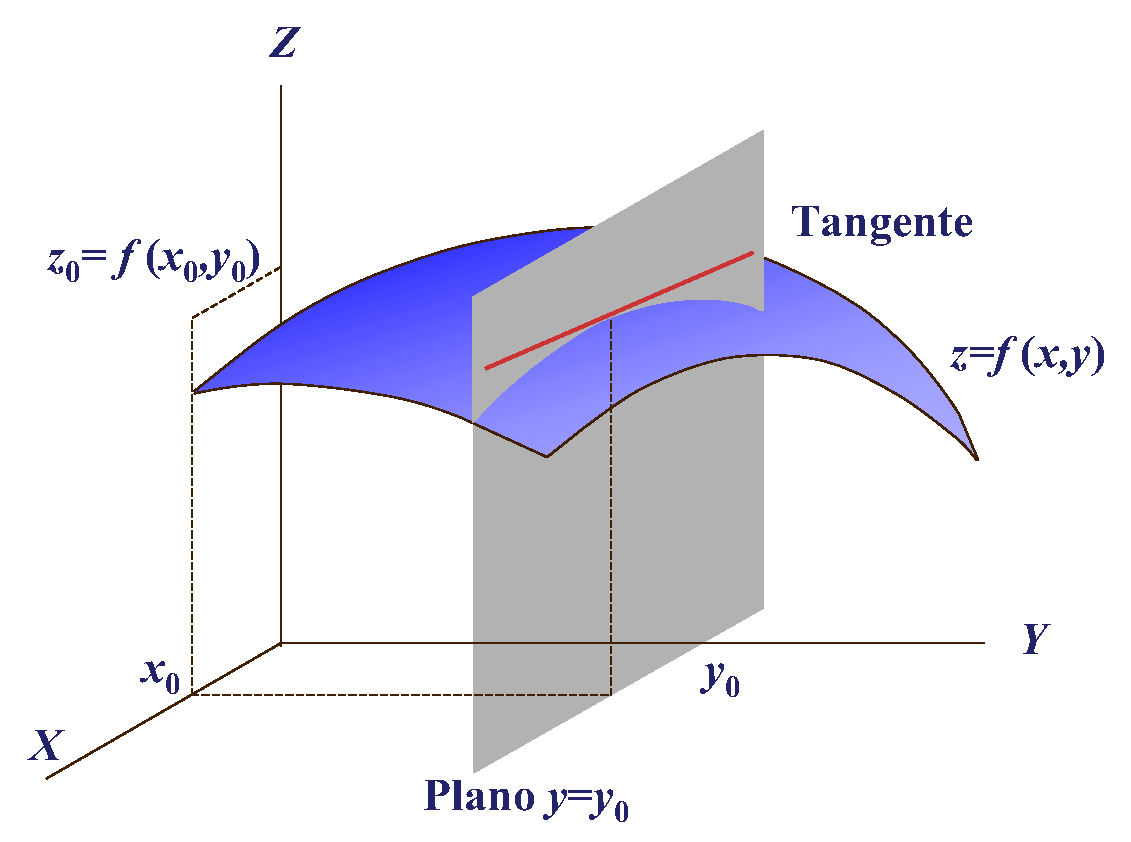
\includegraphics[scale=0.4]{img/derivadas_varias_variables/tangentesuperficie}
\caption{La derivada parcial de una función $f(x,y)$ con respecto a
$x$ en el punto $(x_0,y_0)$, como la pendiente de la recta tangente
a la curva descrita por la intersección de la superficie de $f$ y el
plano de ecuación $y=y_0$.}
\end{center}
\end{figure}


\subsection{Derivadas parciales sucesivas de una función de $n$
variables}

De la misma forma que en las funciones de una variable, mediante los
límites que las definen, siempre y cuando existan, obtenemos las
segundas, terceras y derivadas de cualquier orden. Es decir, si $f$
es una función real de $n$ variables, con sus correspondientes
derivadas parciales, a su vez también las mismas son funciones de
$n$ variables que, en determinadas condiciones, podrán derivarse de
nuevo con respecto a sus $n$ variables para obtener derivadas
parciales segundas, y así sucesivamente hasta órdenes superiores de
derivación.

Para la derivada parcial de segundo orden se utiliza la notación
$f_{x_ix_j}$ ó $\dfrac{{\partial ^2 f}} {{\partial x_j \partial x_i
}}$:


\[
f_{x_i x_j }  = \frac{{\partial ^2 f}} {{\partial x_j \partial x_i
}} = \frac{\partial } {{\partial x_j }}\left( {\frac{{\partial f}}
{{\partial x_i }}} \right)
\]

Por ejemplo, para una función de dos variables $f(x,y)$, tenemos dos derivadas parciales de primer orden, que siguen
siendo funciones de las variables $x$ e $y$:
\[
\frac{\partial f}{\partial x}(x,y)\qquad \frac{\partial f}{\partial y}(x,y) 
\] y cuatro diferentes de segundo orden, que también serán funciones de $x$ e $y$, aunque ya no se
refleje para aligerar la notación:
\[
\frac{\partial}{\partial x}\left({\frac{\partial f}{\partial x}}\right) = \frac{\partial^2 f}{\partial x^2}
\]
\[
\frac{\partial}{\partial y}\left({\frac{\partial f}{\partial x}}\right) = \frac{\partial^2 f}{\partial y\partial x}
\]
\[
\frac{\partial}{\partial x}\left({\frac{\partial f}{\partial y}}\right) = \frac{\partial^2 f}{\partial x\partial y}
\]
\[
\frac{\partial}{\partial y}\left({\frac{\partial f}{\partial y}}\right) = \frac{\partial^2 f}{\partial y^2}
\]

La primera y la última reciben el nombre de derivadas segundas, mientras que la segunda y tercera se denominan derivadas
cruzadas.

Si procedemos con las derivadas parciales de tercer orden tendríamos ocho diferentes, y el número es más amplio con
funciones de tres o más variables.
No obstante, el teorema conocido con \emph{Teorema de Schwartz de las Derivadas Cruzadas} reduce el número de derivadas
parciales diferentes:

\begin{teorema}[Schwartz]
Si $f$ es una función de $n$ variables con derivadas parciales segundas cruzadas continuas en un conjunto abierto que
contiene al punto $a$, entonces en dicho punto se cumple
\[
\frac{\partial ^2 f}{\partial x_i \partial x_j } = \frac{\partial ^2 f}{\partial x_j \partial x_i }
\] 
e igual con las derivadas cruzadas de tercer y superior orden.
\end{teorema}

Es decir, si se cumplen las hipótesis del teorema de Schwartz concluimos que, a efectos de cálculo, tan sólo importa el
número de veces que se deriva respecto a cada variable, pero no el orden de la derivación.

\subsection{Vector gradiente y matriz hessiana}
A partir de las derivadas parciales de primer orden de un campo escalar, podemos definir el siguiente vector:

\begin{definicion}[Vector gradiente]
Dado un campo escalar $f(x_1,\ldots,x_n)$, se llama \emph{gradiente} de $f$, y se escribe $\nabla f$, a la función que a
cada punto $a=(a_1,\ldots,a_n)$ le asigna el vector cuyas coordenadas cartesianas son las derivadas parciales de $f$ en
$a$,
\[
\nabla f(a)=\left(\frac{\partial f}{\partial x_1}(a),\ldots,\frac{\partial f}{\partial x_n}(a)\right).
\]
\end{definicion}

El vector gradiente en un punto dado tiene la misma magnitud y dirección que la velocidad máxima de variación de la
función en ese punto, por lo que $\nabla f(a)$ indica la dirección de máximo crecimiento de $f$ en el punto $a$,
mientras que $-\nabla f(a)$ indica la dirección de máximo decrecimiento.

Y a partir de las derivadas parciales de segundo orden, podemos definir la siguiente matriz:

\begin{definicion}[Matriz hessiana]
Dada una función de varias variables $f(x_1,\ldots,x_n)$, para la que existen todas sus derivadas parciales de segundo
orden en un punto $a=(a_1,\ldots,a_n)$, se define la \emph{matriz hessiana} de $f$ en $a$, y se nota $\nabla^2f(a)$, como la
matriz cuadrada cuyos elementos son
\[
\nabla^2f(a)=\left(
\begin{array}{cccc}
\dfrac{\partial^2 f}{\partial x_1^2}(a) & 
\dfrac{\partial^2 f}{\partial x_1 \partial x_2}(a) &
\cdots &
\dfrac{\partial^2 f}{\partial x_1 \partial x_n}(a)\\
\dfrac{\partial^2 f}{\partial x_2 \partial x_1}(a) &
\dfrac{\partial^2 f}{\partial x_2^2}(a) & 
\cdots &
\dfrac{\partial^2 f}{\partial x_2 \partial x_n}(a)\\
\vdots & \vdots & \ddots & \vdots \\
\dfrac{\partial^2 f}{\partial x_n \partial x_1}(a) &
\dfrac{\partial^2 f}{\partial x_n \partial x_2}(a) &
\cdots &
\dfrac{\partial^2 f}{\partial x_n^2}(a)
\end{array}
\right).
\]
Al determinante de esta matriz se le llama \emph{hessiano} de $f$ en $a$, y se nota $Hf(a)=|\nabla^2f(a)|$.
\end{definicion}

Entre las utilidades de la matriz Hessiana y el hessiano está la determinación de los extremos relativos y los puntos de
silla de una función. 

\subsection{Derivada direccional}
Ya se ha visto que la derivadas parciales miden la tasa de variación instantánea de la función con respecto a cada uno
de sus variables, es decir, en la dirección de cada uno de los ejes de coordenadas. 
Pero, \emph {¿qué pasa si nos movemos en cualquier otra dirección?}
La tasa de variación instantánea de $f$ en un punto $a$ en la dirección de un vector unitario cualquiera $u$ se conoce
como \emph{derivada direccional}.

\begin{definicion}[Derivada direccional]
Dado un campo escalar $f$ de $\mathbb{R}^n$, un punto $a$ y un vector unitario $\mathbf{u}$ en ese espacio, el límite
\[
f'_{\mathbf{u}}(a) = \lim_{h\rightarrow 0}\frac{f(a+h\mathbf{u})-f(a)}{h},
\] 
cuando existe, se llama \emph{derivada direccional} de $f$ en el punto $a$ en la dirección de $\mathbf{u}$.
\end{definicion}
Se cumple 
\[
(f'_{\mathbf{u}}(a) \nabla f(P)\cdot \mathbf{u}.
\]
Obsérvese que las derivadas parciales son las derivadas direccionales en las direcciones de los vectores coordenados.

\subsection{Derivación implícita}
Si se sabe que la ecuación 
\[
f(x,y)=0
\]
define a $y$ como función de $x$, $y=h(x)$, alrededor de cierto valor $x=x_0$ para el que $y=h(x_0)=y_0$, entonces, si se toma la trayectoria $g(x)=(x,h(x))$, la ecuación anterior se puede expresar como
\[
(f\circ g)(x) = f(g(x)) = f(x,h(x))=0,
\]
de modo que usando la regla de la cadena sobre se tiene
\[
(f\circ g)'(x) = \nabla f(g(x))\cdot g'(x) = \left(\frac{\partial f}{\partial x}, \frac{\partial f}{\partial y}\right)\cdot (1,h'(x)) = 
\frac{\partial f}{\partial x}+\frac{\partial f}{\partial y}h'(x) = 0,
\] 
de donde se deduce
\[
y'=h'(x)=\frac{-\dfrac{\partial f}{\partial x}}{\dfrac{\partial f}{\partial y}}
\]

\subsection{Cálculo de extremos}
Si $a$ es un extremo de un campo escalar $f$ de $\mathbb{R}^n$, entonces se cumple que $a$ es un punto crítico de $f$,
es decir,
\[
\nabla f(P) = 0,
\]
Sin embargo, no todos los puntos críticos son extremos relativos. 
Existen puntos como el de la figura~\ref{g:punto_silla} donde se anula el gradiente y que no son puntos de máximo, ni de
mínimo.
Estos puntos se conocen como \emph{puntos de silla}. 
\begin{figure}[htp]
\begin{center}
\scalebox{1}{\psset{unit=0.65}
\psset{viewpoint=50 50 30 rtp2xyz,Decran=50}
\begin{pspicture*}(-7,-4.2)(7,4.3)
%\psSolid[object=grille,base=-4 4 -4 4,action=draw]
\psSurface[fillcolor=blue!50,ngrid=.25 .25,incolor=yellow,algebraic,linewidth=0.25\pslinewidth,linecolor=gray](-2,-2)(2,2){x^2-y^2}
\axesIIID(1,0,0)(4,4,4)
\psPoint(0,0,0){p}
\psdots[linecolor=red](p)
\uput[r](p){$(0,0,0)$ Punto de silla}
\end{pspicture*}}.
\caption{Gráfica de la función $f(x,y)=x^2-y^2$, que tiene un punto de silla en $(0,0)$. }
\label{g:punto_silla}
\end{center}
\end{figure}

Afortunadamente, es posible determinar si un punto crítico es un extremo relativo o un punto de silla a partir de la
matriz Hessiana y el hessiano. 

\begin{teorema}
Dado un punto crítico $a$ de un campo escalar $f$ que tiene matríz hessiana $Hf(a)$, se cumple
\begin{itemize}
\item Si $\nabla^2f(a)$ es definido positivo entonces $f$ tiene un mínimo relativo en $a$.
\item Si $\nabla^2f(a)$ es definido negativo entonces $f$ tiene un máximo relativo en $a$.
\item Si $\nabla^2f(a)$ es indefinido entonces $f$ tiene un punto de silla en $a$.
\end{itemize}
\end{teorema}
En el caso de que $\nabla^2f(a)$ sea semidefinido, no se puede obtener ninguna conclusión y hay que recurrir a derivadas
parciales de orden superior.

En el caso particular de un campo escalar de dos variables se tiene
\begin{teorema}
Dado un punto crítico $a=(x_0,y_0)$ de un campo escalar $f(x,y)$ que tiene matríz hessiana $\nabla^2f(a)$, se cumple
\begin{itemize}
\item Si $Hf(a)>0$ y $\dfrac{\partial^2 f}{\partial x^2}(a)>0$ entonces $f$ tiene un mínimo relativo en $a$.
\item Si $Hf(a)>0$ y $\dfrac{\partial^2 f}{\partial x^2}(a)<0$ entonces $f$ tiene un máximo relativo en $a$.
\item Si $Hf(a)<0$ entonces $f$ tiene un punto de silla en $a$.
\end{itemize}
\end{teorema}

\newpage

\section{Ejercicios resueltos}
\begin{enumerate}[leftmargin=*]
\item Dada la función $f(x,y)=y^2-x^2$, se pide:
\begin{enumerate}
\item Dibujar su gráfica. 
\begin{indicacion}
{\begin{enumerate}
\item Introducir la expresión \comando{f(x,y):=y\^{}2-x\^{}2}.
\item Hacer clic sobre el botón \boton{Ventana 3D} para pasar a la ventana de gráficas 3D.
\item Hacer clic sobre el botón \boton{Representar}).
\end{enumerate}
}
\end{indicacion}

\item Dibujar las curvas de nivel $f(x,y)=k$, para valores enteros de $k$ desde 1 hasta 5.
\begin{indicacion}
{
\begin{enumerate}
\item Introducir la ecuación \comando{f(x,y)=k} para cada valor de $k$.
\item Hacer clic sobre el botón \boton{Ventana 2D} para pasar a la ventana de gráficas 2D.
\item Hacer clic sobre el botón \boton{Representar Expresión}).
\end{enumerate}
}
\end{indicacion}

\item Dibujar el plano $x=1$. ¿Qué figura forma la intersección de este plano con la gráfica de $f$?
\begin{indicacion}
{
\begin{enumerate}
\item Introducir la ecuación del plano \comando{x=1}.
\item Hacer clic sobre el botón \boton{Ventana 3D} para pasar a la ventana de gráficas 3D.
\item Hacer clic sobre el botón \boton{Representar}).
\end{enumerate}
}
\end{indicacion}

\item Calcular la derivada de $f(1,y)$ en $y=2$.
\begin{indicacion}
{
\begin{enumerate}
\item Introducir la expresión \comando{f(1,y)}.
\item Hacer clic sobre el botón \boton{Hallar una derivada}.
\item En el cuadro de diálogo que aparece, hacer clic en el botón \boton{Simplificar}.
\item Hacer clic sobre el botón \boton{Sustituir variables}.
\item En el cuadro de diálogo que aparece introducir el valor 2 y hacer clic en el botón \boton{Simplificar}.
\end{enumerate}
}
\end{indicacion}

\item Dibujar el plano $y=2$. ¿Qué figura forma la intersección de este plano con la gráfica de $f$?
\begin{indicacion}
{
\begin{enumerate}
\item Introducir la ecuación del plano.
\item Hacer clic sobre el botón \boton{Ventana 3D} para pasar a la ventana de gráficas 3D.
\item Hacer clic sobre el botón \boton{Representar}).
\end{enumerate}
}
\end{indicacion}

\item Calcular la derivada de $f(x,2)$ en $x=1$.
\begin{indicacion}
{
\begin{enumerate}
\item Introducir la expresión \comando{f(x,2)}.
\item Hacer clic sobre el botón \boton{Hallar una derivada}.
\item En el cuadro de diálogo que aparece, hacer clic en el botón \boton{Simplificar}.
\item Hacer clic sobre el botón \boton{Sustituir variables}.
\item En el cuadro de diálogo que aparece introducir el valor 1 y hacer clic en el botón \boton{Simplificar}.
\end{enumerate}
}
\end{indicacion}

\item Calcular la derivadas parciales de $f$ en el punto $(1,2)$. ¿Qué conclusiones sacas?
\begin{indicacion}
{
\begin{enumerate}
\item Introducir la expresión \comando{f(x,y)} o seleccionarla en la expresión anterior. 
\item Hacer clic sobre el botón \boton{Hallar una derivada}.
\item En el cuadro de diálogo que aparece, hacer clic en el botón \boton{Simplificar}.
\item Hacer clic sobre el botón \boton{Sustituir variables}.
\item En el cuadro de diálogo que aparece introducir el valor 1 y hacer clic en el botón \boton{Simplificar}.
\end{enumerate}
}
\end{indicacion}
\end{enumerate}


\item  Calcular las siguientes derivadas parciales:
\begin{enumerate}
\item  $\dfrac{\partial }{\partial V}\dfrac{nRT}{V}.$

\begin{indicacion}
{
\begin{enumerate}
\item Introducir la expresión en Derive.
\item Hacer click sobre el \boton{Hallar una derivada}.
\item En el cuadro de diálogo que aparece, en la lista de hipotéticas variables en las que podemos derivar
(evidentemente, para Derive tanto $n$ como $R$ también son variables), seleccionar la variable $V$, introducir el orden
$1$ y hacer clic en el botón \boton{Simplificar}.
\end{enumerate}
}
\end{indicacion}

\item  $\dfrac{\partial ^{2}}{\partial x\partial y}e^{x+y}\ $sen$\ \dfrac{x}{y}.$
\begin{indicacion}
{\begin{enumerate}
\item Introducir la expresión \comando{sin(x)}.
\item Hacer clic sobre el botón \boton{Hallar una derivada}, y en el cudadro de diálogo que aparece
seleccionar la variable $y$ y hacer clic en el botón \boton{Simplificar}.
\item Una vez obtenida primera derivada con respecto a $y$, para obtener la segunda con respecto a $x$, seleccionamos la
expresión obtenida en el apartado anterior y volvemos a repetir el proceso pero seleccionando la variable
$x$.
\end{enumerate}
}
\end{indicacion}
\end{enumerate}

\item Dada la función $f(x,y)=20-4x^2-y^2$, se pide calcular en el punto $(2,-3)$:
\begin{enumerate}
\item Vector gradiente.
\begin{indicacion}{
\begin{enumerate}
\item Definir la función introduciendo la expresión \comando{f(x,y):=20-4x\^{}2-y\^{}2}.
\item Introducir la expresión \comando{f'(2,-3)}.
\item Hacer clic en el botón \boton{Simplificar}.
\end{enumerate}
}
\end{indicacion}

\item Matriz hessiana.
\begin{indicacion}{
\begin{enumerate}
\item Introducir la expresión \comando{f''(2,-3)}.
\item Hacer clic en el botón \boton{Simplificar}.
\end{enumerate}
}
\end{indicacion}

\item Calcular el determinante hessiano.
\begin{indicacion}{
\begin{enumerate}
\item Introducir la expresión \comando{DET(f''(2,-3))}.
\item Hacer clic sobre el botón \boton{Simplificar}.
\end{enumerate}
}
\end{indicacion}
\end{enumerate} 


\item Dada la función
\[
f(x,y,z)=\sen((x^2-y^2)z)
\]
\begin{enumerate}
\item Definir la función.
\begin{indicacion}
{Introducir la expresión \comando{f(x,y,z):=sin((x\^{}2-y\^{}2)z)}.
}
\end{indicacion}

\item Calcular su vector gradiente en el punto $(0,-1,\pi/2)$.
\begin{indicacion}{
\begin{enumerate}
\item Introducir la expresión \comando{f'(0,-1,pi/2)}.
\item Hacer clic sobre el botón \boton{Simplificar}.
\end{enumerate}
}
\end{indicacion}

\item Calcular su matriz Hessiana en el punto $(0,-1,\pi/2)$.
\begin{indicacion}{
\begin{enumerate}
\item Introducir la expresión \comando{f''(0,-1,pi/2)}.
\item Hacer clic sobre el botón \boton{Simplificar}.
\end{enumerate}
}
\end{indicacion}

\item Comprobar que se cumple el teorema Schwartz de las derivadas para las derivas cruzadas:
\begin{enumerate}
\item $\dfrac{{\partial ^3 f}} {{\partial x\partial z\partial y}}$
\begin{indicacion}
{\begin{enumerate}
\item Introducir la expresión \comando{f(x,y,z)}.
\item Hacer clic sobre el botón \boton{Hallar una derivada}.
\item En el cuadro de diálogo que aparece seleccionar la variable $y$ y hacer clic en el botón \boton{Simplificar}.
\item Repetir el proceso con la expresión resultante, seleccionando esta vez la variables $z$.
\item Repetir una vez más el proceso con la expresión resultante, seleccionando esta vez la variables $x$.
\end{enumerate}
}
\end{indicacion}

\item $\dfrac{{\partial ^3 f}} {{\partial z\partial x\partial y}}$
\begin{indicacion}
{\begin{enumerate}
\item Introducir la expresión \comando{f(x,y,z)}.
\item Hacer clic sobre el botón \boton{Hallar una derivada}.
\item En el cuadro de diálogo que aparece seleccionar la variable $y$ y hacer clic en el botón \boton{Simplificar}.
\item Repetir el proceso con la expresión resultante, seleccionando esta vez la variables $x$.
\item Repetir una vez más el proceso con la expresión resultante, seleccionando esta vez la variables $z$.
\end{enumerate}
}
\end{indicacion}
\end{enumerate}

¿Puedes predecir el valor de $\dfrac{{\partial ^3 f}} {{\partial y\partial x\partial z}}$?
\end{enumerate}

\item Hallar la recta normal a la superficie $S: x+2y-\log z +4 =0$ en el punto $(0,-2,1)$ y dibujarla.
\begin{indicacion}
{Para dibujar la gráfica de la superficie:
\begin{enumerate}
\item Introducir la expresión \comando{z=exp(x+2y+4)}.
\item Hacer clic en el botón \boton{Ventana 3D} para pasar a la ventana gŕafica 3D.
\item Hacer clic en el botón \boton{Representar}.
\end{enumerate}
Para dibujar la gráfica de la recta normal:
\begin{enumerate}[resume]
\item Hacer clic en el botón \boton{Activar la ventana de Álgebra} para pasar a la ventana de expresiones.
\item Definir la función introduciendo la expresión \comando{f(x,y,z):=x+2y-log z+4}.
\item Introducir la expresión \comando{[0,-2,1]+tf'(0,-2,1)}.
\item Hacer clic en botón \boton{Simplificar}.
\item Hacer clic en el botón \boton{Ventana 3D} para pasar a la ventana gŕafica 3D.
\item Hacer clic en el botón \boton{Representar}.
\end{enumerate}
}
\end{indicacion}

\item La ecuación $x+y-2e^y+2=0$ define implícitamente una función $y=f(x)$ alrededor del punto $(0,0)$. Calcular
$f'(0)$.
\begin{indicacion}
{\begin{enumerate}
\item Introducir la expresión \comando{x+y-2\#e\^{}y+2}.
\item Hacer clic sobre el botón \boton{Hallar una derivada}.
\item En el cuadro de diálogo que aparece seleccionar la variable $x$ y hacer clic en el botón \boton{Simplificar}. 
\item Seleccionar de nuevo la expresión inicial.
\item Hacer clic sobre el botón \boton{Hallar una derivada}.
\item En el cuadro de diálogo que aparece seleccionar la variable $y$ y hacer clic en el botón \boton{Simplificar}.
\item Introducir la expresión \comando{-\#i/\#j} donde \comando{\#i} es la etiqueta de la expresión de la derivada
parcial con respecto a $x$ y \comando{\#j} es la etiqueta de la expresión de la derivada parcial con respecto a $y$.
\item Hacer clic sobre el botón \boton{Sustituir}.
\item En el cuadro de diálogo que aparece, seleccionar $x$ e introducir el valor $0$, seleccionar $y$ e
introducir el valor $0$, y hacer clic en el botón \boton{Simplificar}.
\end{enumerate}
}
\end{indicacion}

\item Calcular la derivada direccional de la función $h(x,y)= 3x^2+y$ en el punto $(0,0)$, en la dirección del vector
$(1,1)$.
\begin{indicacion}
{\begin{enumerate}
\item Definir la función introduciendo la expresión \comando{f(x,y):=3x\^{}2+y}.
\item Introducir la expresión \comando{f'(0,0)SIGN([1,1])}.
\item Hacer clic en el botón \boton{Simplificar}.
\end{enumerate}
}
\end{indicacion}

\item Dada la función $f(x,y)=x^3+y^3-3xy$, se pide:
\begin{enumerate}
\item Definirla y dibujar su gráfica. ¿Puedes identificar a simple vista sus extremos relativos?
\begin{indicacion}
{\begin{enumerate}
\item Definir la función introduciendo la expresión \comando{f(x,y):=x\^{}3+y\^{}3-3xy}.
\item Hacer clic sobre el botón \boton{Ventana 3D} para pasar a la ventana de gráficas 3D.
\item Hacer clic sobre el botón \boton{Representar}).
\end{enumerate}
}
\end{indicacion}

\item Calcular los puntos críticos que anulan el vector gradiente de $f$. 
\begin{indicacion}
{\begin{enumerate}
\item Introducir la expresión \comando{f'(x,y)}.
\item Hacer clic en el botón \boton{Simplificar}.
\item Hacer clic en el botón \boton{Resolver o despejar}.
\item Seleccionar ambas variables $x$ e $y$, seleccionar el dominio Real y hacer clic en el botón \boton{Resolver}.
\end{enumerate}
}
\end{indicacion}

\item Determinar los extremos relativos y los puntos de silla de $f$.
\begin{indicacion}
{\begin{enumerate}
\item Introducir la expresión \comando{f''(x,y)}, para $(x,y)$ el primer punto crítico.
\item Hacer clic en el botón \boton{Simplificar}.
\item Introducir la expresión \comando{DET(\#i)}, donde \comando{\#i} es la etiqueta de la expresión de la matriz
hessiana anterior.
\item Hacer clic sobre el botón \boton{Simplificar}.
\item Repetir el mismo procedimiento con el segundo punto crítico. 
\end{enumerate}
}
\end{indicacion}
\end{enumerate}

\end{enumerate}


\section{Ejercicios propuestos}

\begin{enumerate}[leftmargin=*]

\item Una nave espacial está en problemas cerca del sol. 
Se encuentra en la posición $(1,1,1)$ y la temperatura de la nave cuando está en la posición $(x,y,z)$ viene dada por
$T(x,y,z)=\mbox{e}^{-x^2-2y^2-3z^2}$ donde $x,y,z$ se miden en metros.
¿En qué dirección debe moverse la nave para que la temperatura decrezca lo más rápidamente posible?

\item Calcular el vector gradiente, la matriz hessiana y el hessiano de la función
\[
g(x,y) = \frac{x}{\sqrt{x^2+y^2+z^2}^3}
\]
en el punto $(1,1,1)$ y en el punto $(0,3,4)$. 

\item Obtener los puntos del elipsoide $S: x^2+2y^2+z^2=1$ en los que el plano tangente es paralelo al plano $\Pi:
x-y+2z^2=0$.

\item Estudiar los extremos relativos de la función 
\[
f(x)=-\frac{y}{9+x^2+y^2}.
\]

\item Calcular la derivada direccional del campo escalar $f(x,y,z)=x^2-y^2+xyz^3-zx$ en el punto $(1,2,3)$ y en la
dirección del vector $(1,-1,0)$.
\end{enumerate}
%%$HeadURL: https://practicas-derive.googlecode.com/svn/trunk/funciones_elementales.tex $
%$LastChangedDate: 2008-12-08 17:44:27 +0100 (lun, 08 dic 2008) $
%$LastChangedRevision: 4 $
%$LastChangedBy: asalber $

\chapter{Funciones de varias variables:\\ Límites y continuidad}

\section*{Fundamentos Teóricos}
En muchas situaciones prácticas, el valor de una función depende
del que toman todo un conjunto de variables y no ya tan sólo de
una. El objetivo de esta práctica es el de, además de definir
dicho tipo de funciones, introducir algunos de los conceptos
básicos que se refieren a las mismas: gráfica, conjuntos de nivel,
límites y continuidad. Todo ello como extensión de las
definiciones, propiedades y conceptos ya manejados para funciones
de una única variable.

\subsection*{Función real de $n$ variables}
Una función real de varias, $n$, variables es una aplicación que
asigna a cada punto $\vec{x}$ de un conjunto $A$ contenido en
$\mathbb{R}^n$, $ \vec x  = \left( {x_1 ,x_2 ,...,x_n } \right)$,
un único número real $f\left( {\vec x } \right) = f\left( {x_1
,x_2 ,...,x_n } \right)$


\[
f:\begin{array}{*{20}c}
   {A \subset \mathbb{R}^n  \to \mathbb{R}}  \\
   {\vec x  \to f\left( {\vec x } \right)}  \\

 \end{array}
\]

El conjunto $A$ se llama \emph{Dominio} de la función y los
valores de $f$ constituyen el \emph{Rango o Recorrido}.

De $f$ se dice que es una \emph{Función Real de Variable
Vectorial}, y también que se trata de un \emph{Campo Escalar}.
Esto último sobre todo en problemas de Física, en los que abundan
ejemplos de este tipo de funciones: la temperatura como función de
las coordenadas del punto, $T(x,y,z)$; la presión en el seno de un
fluido con idénticas variables, $P(x,y,z)$; o el potencial
eléctrico también como $V(x,y,z)$, entre otros.

\subsection*{Gráfica de una función real de $n$ variables}

Recordemos que la gráfica de una función de una única variable,
$f: A \subset \mathbb{R}  \to \mathbb{R}$, es un subconjunto de
$\mathbb{R}^2$ que consta de todos los puntos $(x,f(x))$. De igual
forma se define la \emph{Gráfica de una Función Real de Variable
Vectorial}, $f: A \subset \mathbb{R}^n  \to \mathbb{R}$, como el
subconjunto de $\mathbb{R}^{n+1}$ que consta de todos los puntos $
\left( {\vec x ,f\left( {\vec x } \right)} \right)$.

\begin{figure}[h!]
\begin{center}
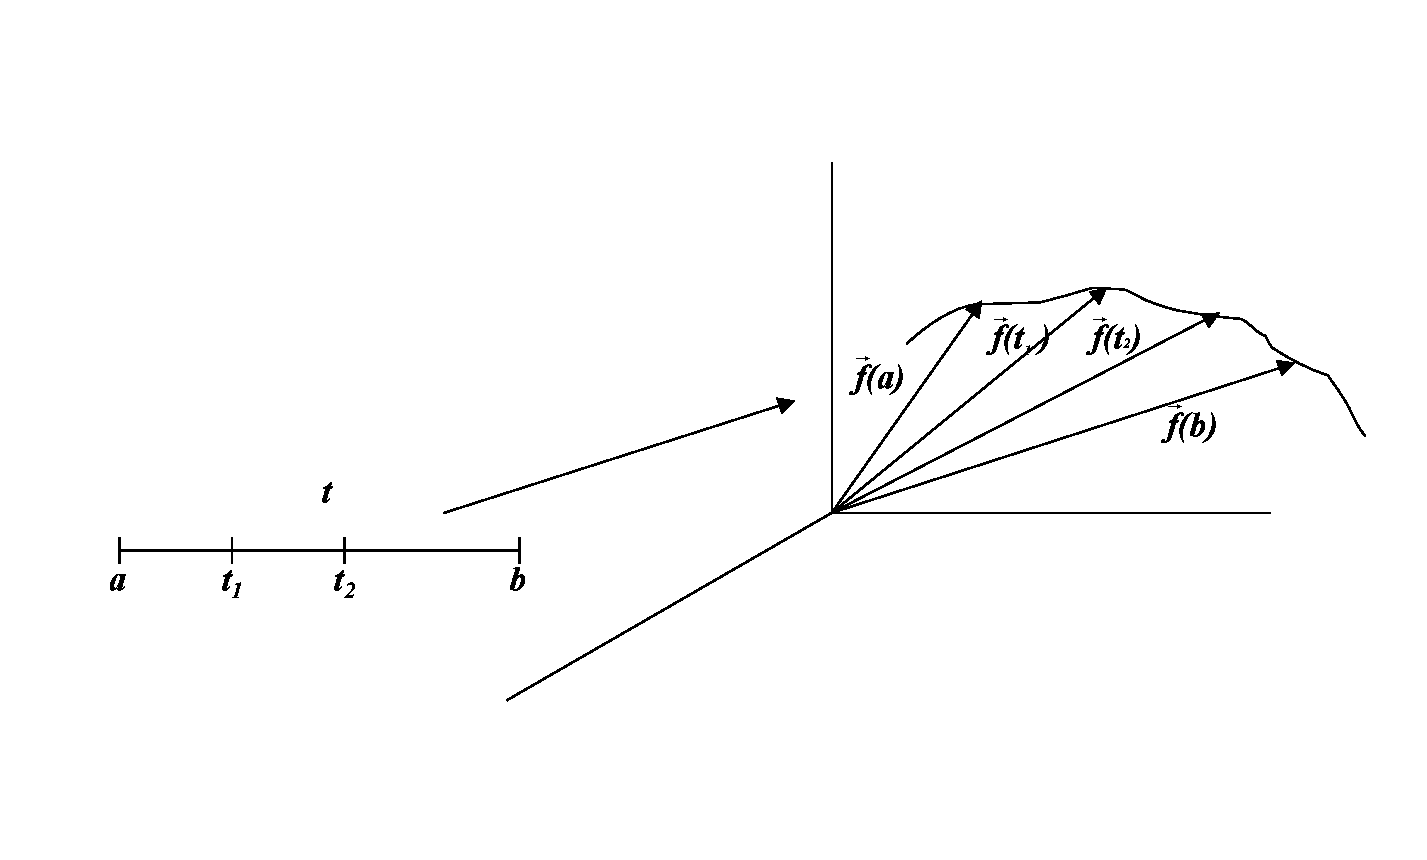
\includegraphics[scale=0.4]{img/limites_varias_variables/grafica}
\caption{Gráfica de una función de dos variables}
\end{center}
\end{figure}


Por ejemplo, si $f$ es una función de dos variables, $f(x,y)$, la
gráfica de $f$ es una superficie en $\mathbb{R}^3$ compuesta por
los puntos $(x,y,f(x,y))$, o de otra forma $(x,y,z)$, donde
$z=f(x,y)$. Además, cualquiera de los programas de Cálculo para
ordenador ofrecen ya la posibilidad de representar las gráficas
``tridimensionales" de funciones de dos variables, proyectadas en
el plano de la pantalla. Para funciones de tres o más variables no
hay un reflejo gráfico para la gráfica de una función, ya que
necesitaríamos cuatro o más coordenadas.




\subsection*{Conjunto de nivel de una función real de $n$
variables}

Sea $f: A \subset \mathbb{R}^n  \to \mathbb{R}$ una función real
de varias variables, y sea $c \in \mathbb{R}$ una constante.
Definimos el \emph{Conjunto de Nivel de Valor $c$} como aquellos
puntos $\vec x  \in A$ para los cuales $f\left( {\vec x } \right)
= c$.

En el caso de las funciones de dos variables, $f(x,y)$, el
conjunto de nivel recibe el nombre de curva de nivel. Por lo
tanto, la Curva de Nivel $c$ de la superficie $z=f(x,y)$ es el
conjunto formado por los puntos del plano $(x,y)$ pertenecientes
al dominio de $f$ tales que  $f(x,y)=c$.

El ejemplo más frecuente de curvas de nivel aparece en los mapas
topográficos. Si consideramos que $z=f(x,y)$ es la altura sobre el
nivel de mar del punto de coordenadas $(x,y)$, y unimos en el
plano los puntos de igual altura, obtenemos unas curvas que
permiten observar la situación de montañas y valles. Otro ejemplo
de curvas de nivel lo encontramos en los mapas con las
predicciones del tiempo, que presentan las isobaras que surgen al
unir en el plano los puntos de igual presión.

\begin{figure}[h!]
\begin{center}
\includegraphics[scale=0.4]{img/limites_varias_variables/conjuntonivel}
\caption{Conjunto de nivel de una función de dos variables}
\end{center}
\end{figure}


\subsection*{Límite de una función real de $n$ variables}

Sea $f: A \subset \mathbb{R}^n  \to \mathbb{R}$ y un punto $\vec
a$ de $\mathbb R^n$, que no tiene necesariamente que pertenecer al
dominio de $f$ con tal de que sea punto de acumulación del mismo
(es decir, sí que deben existir puntos de $A$ tan próximos como se
quiera a $\vec a$). Entonces, de forma similar a lo que sucedía
con las funciones de una única variable, y de manera informal,
decimos que:

\[
\mathop {\lim }\limits_{\vec x \to \vec a} f\left( {\vec x}
\right)=l
\]
si $f\left( {\vec x} \right)$ se aproxima cada vez más a $l$ a
medida que $\vec x$ se aproxima a $\vec a$.

No obstante, en $\mathbb R^n$ el concepto de tendencia o
aproximación es mucho más complejo que en $\mathbb R$, ya que para
un cierto $a \in \mathbb R$ tan sólo se puede tender al mismo
desde valores mayores, y hablaríamos de límite por la derecha, o
desde valores menores, y hablaríamos de límite por la izquierda;
mientras que, por ejemplo, en $\mathbb R^2$ podríamos aproximarnos
al punto $\vec a$ de coordenadas $(x_0,y_0)$ a través de infinitas
rectas diferentes, e incluso a través de infinitas curvas
(parábolas, exponenciales, ...); e igual sucedería en cualquier
otro $\mathbb R^n$.

Lo anterior da lugar al siguiente importante teorema, de contenido
similar al que en $\mathbb R$ afirma que el límite existe si
existen los límites laterales y coinciden:


\begin{teorema}
Si existe el límite de $f: A \subset \mathbb{R}^n  \to \mathbb{R}$
en el punto $\vec a$ y vale $l$, entonces existe el límite sea
cual fuere la forma de tender hacia $\vec a$ y vale $l$.
\end{teorema}

Lo anterior puede utilizarse para demostrar la no existencia del
límite, sin más que considerar dos tendencias diferentes y ver que
los límites que se obtienen no son iguales. Sin embargo, no puede
utilizarse para demostrar la existencia del mismo, ya que habría
que considerar las infinitas tendencias diferentes. Por ello, el
cálculo de límites de funciones de dos o más variables resulta
complejo y difícil de plasmar en un algoritmo, lo cual se traduce
en que los programas actuales de Cálculo con ordenador realizan
correctamente tan sólo algunos de los límites de funciones de este
tipo.

Mucho más fácil que el cálculo del límite de una función de varias
variables, resulta el cálculo de los denominados \emph{Límites
Iterados}, también llamados \emph{Reiterados o Sucesivos}, que
definimos a continuación:

Sea $f: A \subset \mathbb{R}^n  \to \mathbb{R}$, $\vec x \in A$ un
punto del dominio de coordenadas $\left(x_1,x_2,...,x_n\right)$, y
$\vec a=\left(a_1,a_2,...,a_n\right)$ el punto al que tendemos. Se
definen los límites iterados si existe:

\[
\mathop {\lim }\limits_{x_1  \to a_1 } \left( {\mathop {\lim
}\limits_{x_2  \to a_2 } \left( {...\left( {\mathop {\lim
}\limits_{x_n  \to a_n } f\left( {\vec x} \right)} \right)}
\right)} \right)
\]
y todas las reordenaciones de los diferentes límites.

Por ejemplo, en $\mathbb R^2$: $\vec x=(x,y)$, $\vec a=(x_0,y_0)$;
y resultan dos posibles límites iterados:


\[
\mathop {\lim }\limits_{x \to x_0 } \left( {\mathop {\lim
}\limits_{y \to y_0 } f(x,y)} \right)
\]

\[
\mathop {\lim }\limits_{y \to y_0 } \left( {\mathop {\lim
}\limits_{x \to x_0 } f(x,y)} \right)
\]

De nuevo, podría demostrarse que si existe $ \mathop {\lim
}\limits_{\vec x \to \vec a} f\left( {\vec x} \right)$ y los
límites reiterados de $f$, entonces todos coinciden. Lo cual nos
permite asegurar que si los límites reiterados de una función en
un punto $\vec x =\vec a$ existen y son diferentes, entonces no
existe $ \mathop {\lim }\limits_{\vec x \to \vec a} f\left( {\vec
x} \right)$.

\subsection*{Continuidad de una función real de $n$ variables}

De manera similar a lo que secede con las funciones de una única
variable, $f: A \subset \mathbb{R}^n  \to \mathbb{R}$ se dice que
es \emph{Continua en el Punto} $\vec a \in A$ si se verifican:

\begin{itemize}
  \item Existe $f\left(\vec a\right)$.
  \item Existe $\mathop {\lim }\limits_{\vec x \to \vec a} f\left( {\vec x}
\right)=l$.

\item Ambos coinciden: $f\left(\vec a\right)=l$.
\end{itemize}

Y diríamos que $f$ es continua en todo un subconjunto de su
dominio si es continua en todos los puntos del mismo.

Si tenemos una función de dos variables, $f(x,y)$, la continuidad
en un conjunto significaría geométricamente que la superficie
$z=f(x,y)$ no tiene saltos ni agujeros en todo el conjunto.





\section{Ejercicios resueltos}

\begin{enumerate}[leftmargin=*]
\item Dada la función:

\[
f(x,y) = \frac{1} {{x^2  + 2y^2  + 1}}
\]

\begin{enumerate}
  \item Definirla y representar su gráfica. Una vez representada,
  rotarla, agrandarla, contraerla, hacer zoom hacia fuera y hacia
  dentro para cambiar la escala de representación, y cambiar el
  número de paneles para representar la gráfica con una trama más
  o menos tupida.

\begin{indicacion}
{

\begin{enumerate}

\item Para definirla, utilizar el operador definición $:=$, y para
representarla, utilizar el botón \boton{Ventana 3D}, y una vez en el
entorno tridimensional, utilizar el botón \boton{Representar}.

\item

\begin{itemize}

\item Para rotarla, utilizar los botones \boton{Rota la gráfica},
\boton{Girar hacia la izquierda}, \boton{Girar hacia la derecha},
\boton{Rotar hacia arriba} y \boton{Rotar hacia abajo}.

\item Para agrandarla y contraerla utilizar los botones
\boton{Magnificar} y \boton{Contraer}. Observar cómo, tanto al
agrandar como al contraer, no cambiamos la escala del cubo en el que
se muestra la gráfica, y por tanto seguimos viendo la misma porción
de gráfica alejada o acercada.

\item Un efecto similar al que se genera mediante la rotación de
la gráfica, combinada con un acercamiento o alejamiento, lo podemos
obtener mediante el botón \boton{Fijar la posición del ojo}.

\item Para hacer zoom hacia fuera o hacia dentro utilizar los
botones \boton{Zoom hacia fuera} y \boton{Zoom hacia dentro}.
Comprobar cómo varía la escala del cubo en el que se muestra la
gráfica al hacer zoom. En definitiva, cambiamos la porción de
gráfica que vemos, pero no la posición desde la que la miramos. Un
efecto similar se obtiene con los botones \boton{Ajuste del
mínimo/máximo} y \boton{Restablece rango}.

\item Para cambiar el entramado de la gráfica, lo más cómodo es
utilizar el menú contextual que aparece al pulsar el botón derecho
del ratón sobre la gráfica y utilizar \menu{Editar->Parámetros de la
gráfica->Número de Paneles}.
\end{itemize}

\end{enumerate}

}
\end{indicacion}

  \item Representar la curva de nivel que se obtiene para
  $f(x,y)=1/2$.

\begin{indicacion}
{Igualar la definición de la función a 1/2 y representar mediante el
botón \boton{Ventana 2D}. Recordar que las curvas de nivel son
puntos del plano $XY$ en los que la función toma el mismo valor (la
gráfica tridimensional presentaría igual altura).

}
\end{indicacion}


  \item Utilizar la función \comando{VECTOR(u,k,m,n)} para dibujar todas las
  curvas de nivel de la forma $f(x,y) = 1/k$, donde $k$ toma los
  valores naturales de $2$ a $10$ (tener en cuenta que, en la función \comando{Vector},
  $u$ sería la expresión de las curvas de nivel $f(x,y) = 1/k$, y
$k$ un índice de variación que toma valores entre $m$ y $n$).

\begin{indicacion}
{

\begin{enumerate}

\item La función \comando{VECTOR} de Derive, genera un
vector cuyas componentes son la función $u$, que depende de un
índice $k$, variando el mismo entre los valores $m$ y $n$. En
nuestro caso, si introducimos en Derive el comando:

\begin{center}
\comando{VECTOR}$(f(x,y)=1/k,k,2,10)$
\end{center}

se genera un vector cuyas 9 componentes son:
\[
[f(x,y)=1/2,f(x,y)=1/3,...,f(x,y)=1/10]
\]

\item Para representar a la vez todas esas curvas de nivel
generadas, simplemente marcamos la expresión que las contiene, y
procedemos a representar en la \boton{Ventana 2D} de igual forma que
representaríamos cualquier función de una única variable.
\end{enumerate}

}
\end{indicacion}

\end{enumerate}

\item Dada la función:


\[
f(x,y) = \frac{{xy}} {{x^2  + 3y^2 }}
\]

\begin{enumerate}
  \item Definirla y representar su gráfica. Observar
  la gráfica desde diferentes perspectivas,
  con especial interés por lo que ocurre en las
  cercanías del punto (0,0).

\begin{indicacion}
{Para definirla, utilizar el operador de definición :=, y para
cambiar la perspectiva con el objetivo de observar lo que ocurre en
las cercanías del punto (0,0), utilizar los botones
\boton{Magnificar} y los de \boton{Rotación} (hacia arriba y hacia
abajo) y de \boton{Giro} (a izquierda y derecha), además de cambiar
el número de paneles que se muestran por defecto, con el menú
contextual (botón derecho del ratón) y \menu{Editar->Parámetros de
la Gráfica->Número de paneles}.

}
\end{indicacion}

  \item ¿Se puede calcular el valor de la función en el punto
  (0,0)? ¿Puede la función ser continua en (0,0)?.

\begin{indicacion}
{

\begin{enumerate}

\item Para ver cuál es el valor de la función en el punto $(0,0)$,
intentar obtener $f(0,0)$.

\item Para responder a la pregunta sobre si la función puede ser
continua en $(0,0)$, simplemente considerar que la función no está
definida en dicho punto, con lo cual, difícilmente puede ser
continua.

\end{enumerate}

}
\end{indicacion}


  \item Calcular los límites iterados en $(0,0)$. A la vista de
  dichos límites, ¿qué concluimos sobre la existencia, si es que existe, y el valor
  de $\mathop {\lim }\limits_{\left( {x,y} \right) \to \left( {0,0}
  \right)} f\left( {x,y} \right)$?

\begin{indicacion}
{




\begin{enumerate}

\item Para calcular los límites iterados, tomar el límite (botón
\boton{Calcular un límite}) de la función inicialmente considerando
como variable $x$, y luego proceder a calcular el límite del límite
anterior pero ahora tomando como variable $y$:

\[
\mathop {\lim }\limits_{y \to 0 } \left( {\mathop {\lim
}\limits_{x \to 0 } f(x,y)} \right)
\]

Repetir el mismo proceso pero intercambiando las variables, es
decir, inicialmente el límite con respecto a $y$ y luego con
respecto a $x$:

\[ \mathop {\lim }\limits_{x \to 0 } \left( {\mathop {\lim
}\limits_{y \to 0 } f(x,y)} \right)
\]

\item Sobre la existencia del límite de la función, recordar que
para que el límite exista los iterados deben existir y coincidir,
pero se trata de una condición necesaria aunque no suficiente. Por
lo tanto, si los límites iterados no existen, o si existen pero
son diferentes, concluimos que no existe el límite; pero si
existen y son iguales, no podemos concluir que el límite exista.

\end{enumerate}

}
\end{indicacion}


  \item Calcular sus límites direccionales en el mismo punto a través de la familia
  de rectas $y=mx$. A la vista de los resultados, ¿qué concluimos
  sobre la posible existencia del límite en dicho punto?.

\begin{indicacion}
{Para calcular los límites direccionales a través de la familia de
rectas $y=mx$:

\begin{enumerate}

\item En la definición de la función sustituir $y$ por $mx$.

\item Calcular el límite cuando $x$ tiende a 0 de la expresión
resultante (botón \boton{Calcular un límite}). Observar que la
función resultante no depende de $x$ y, por lo tanto, el programa no
propone $x$ como variable en la que calcular el límite (tan sólo
propone $m$). No obstante, podemos poner $x$ en el cuadro de diálogo
mediante el teclado.

\item Como el límite final resultante depende de $m$ quiere ello
decir que el valor del límite depende de la pendiente de la recta
$y=mx$, es decir, es diferente según diferentes tendencias hacia
el punto, lo cual implica que no existe el límite.

\end{enumerate}

}
\end{indicacion}


\end{enumerate}

\item Dada la función:

\[
f(x,y) = \left\{ {\begin{array}{*{20}c}
   0 & {\text{si}} & {x <0}  \\
   \cos{(x^2+y^2)}& {\text{si}} & {x\geq 0}  \\

 \end{array} } \right.
\]

\begin{enumerate}
  \item Utilizar la función condicional de Derive $\comando{If(condicion,opcion 1,opcion 2)}$,
   para definir la función $f(x,y)$.


\begin{indicacion}
{Para la función $f(x)$, podemos, para su definición, utilizar la
función condicional de Derive \comando{If(condición,opción 1,opción
2)}, de tal forma que si se cumple la \comando{condición} el
programa realizará la \comando{opción 1}, y si no se cumple
realizará la \comando{opción 2}. La función condicional de Derive,
\comando{If}, entre otras muchas posibilidades sirve para introducir
funciones definidas a trozos. En nuestro caso la \comando{condición}
es $x<0$, la \comando{opción 1} es $0$, y la \comando{opción 2} es
$\cos(x^2+y^2)$.

Así, la función $f(x,y)$ puede definirse mediante:

\[
f(x,y):=\comando{IF}(x<0,0,\cos(x^2+y^2))
\]

}
\end{indicacion}


  \item Representar su gráfica. A la vista de la gráfica, ¿crees
  que la función será continua en $x=0$?.


\begin{indicacion}
{Para representar la gráfica, botón \boton{Ventana 3D}, y una vez en
el entorno de dibujo de funciones de dos variables, botón
\boton{Representar}. Convendrá editar la gráfica (botón derecho del
ratón sobre la gráfica y menú \menu{Editar}) y aumentar el número de
paneles. }
\end{indicacion}


  \item Demostrar que la función no es continua en $(x,y)=(0,0)$.

\begin{indicacion}
{Se puede demostrar tomando límites en el punto $(0,0)$ a través
de rectas de la forma $y=mx$. Por ejemplo se puede tomar la recta
$y=0$ y ver qué sucede cuando $x$ tiende a cero por la derecha
(por los mayores que 0), o por la izquierda (por los menores que
0).


}
\end{indicacion}


\end{enumerate}
\end{enumerate}


\section{Ejercicios propuestos}
\begin{enumerate}

\item Para la función:

\[
f(x,y) = 10 - \sqrt {x^2  + y^2 }
\]

\begin{enumerate}
\item Representar su gráfica. A la vista de la gráfica, ¿qué forma
tendrán sus curvas de nivel?.

\item Representar sus curvas de nivel para la $f(x,y)=k$, donde
$k$ toma los valores naturales desde 1 hasta 5.
\end{enumerate}

\item Demostrar que no existe el límite:

\[
\mathop {\lim }\limits_{\left( {x,y} \right) \to \left( {0,0}
\right)} \frac{{\left( {x - y} \right)^2 }} {{x^2  + y^2 }}
\]

\item Sea la función:

\[
f(x,y) = \left\{ {\begin{array}{*{20}c}
   {\dfrac{{x^2 }}
{{x^2  + y^2 }}} & {\text{si}} & {\left( {x,y} \right) \ne \left( {0,0} \right)}  \\
   0 & {\text{si}} & {\left( {x,y} \right) = \left( {0,0} \right)}  \\

 \end{array} } \right.
\]

Estudiar su continuidad en todo $\mathbb{R}^2$ (para definirla,
utilizar la función condicional \comando{If}, y para introducir la
\comando{condición} $(x,y)=(0,0)$ utilizar $x=0$ \comando{and}
$y=0$).
\end{enumerate} 
\end{document}
